\documentclass[10pt,xcolor=x11names,compress, notes=show]{beamer}% pour l'impression, tout n'apparait qu'une fois \documentclass[handout,12pt]{beamer}

%\documentclass[xcolor=x11names]{beamer}
%\usepackage[scaled]{helvet}
\usepackage[round]{natbib}



\usepackage[utf8x]{inputenc}
\usepackage{ucs}
\usepackage[french]{babel}
\usepackage{todonotes}
\usepackage{tikz}
\usepackage{color}
%\usepackage{subfigure}
%\usepackage[]{geometry}
\usepackage{changepage}
\usetikzlibrary{calc}

\usepackage{bm}
\usepackage{pifont} %pour les symbole sympa \ding{nb}
\usepackage[export]{adjustbox}
\usepackage{subcaption}

\usepackage{pdfpages}


\setbeamertemplate{navigation symbols}{} 


%\usepackage{palatino}

%pour le theme
%\usetheme{CambridgeUS}

%\usetheme{Goettingen}
\useinnertheme{default}
\useoutertheme[subsection=false]{miniframes}
\setbeamertemplate{blocks}[rounded][shadow=true]
\setbeamercolor{block title}{fg=DeepSkyBlue4,bg=DeepSkyBlue4!10}
\setbeamercolor{block title alerted}{bg=DeepSkyBlue4!0} 
\setbeamercolor{block title example}{bg=DeepSkyBlue4!20}
\setbeamercolor*{lower separation line head}{bg=DeepSkyBlue4} 

\setbeamerfont{title like}{shape=\scshape}
\setbeamercolor{frametitle}{fg=DeepSkyBlue4}
\setbeamercolor{title}{fg=DeepSkyBlue4}
\setbeamercolor{itemize item}{fg=black}
\setbeamercolor{itemize subitem}{fg=black}
\setbeamercolor{toc}{fg=DeepSkyBlue4}
\usepackage{amsmath,mathtools}
\usefonttheme[onlymath]{serif}

\setbeamertemplate{frametitle}{\vspace{0.13cm}\hspace{-0.9cm} \insertframetitle}
\setbeamerfont{frametitle}{size=\Large}

\setlength{\fboxrule}{1pt}

\setbeamertemplate{bibliography item}[]

%couleur table des matières
\usepackage{hyperref}
\hypersetup{colorlinks=true, linkcolor=DeepSkyBlue4}

\setbeamertemplate{caption}{\raggedright\insertcaption\par}

%Mettre la section courante en titre de diapo (pour champ de titre non-vide)
%\addtobeamertemplate{frametitle}{\frametitle{\insertsubsectionhead}}{}

\addtobeamertemplate{footline}{\hspace{11cm} \insertframenumber/\inserttotalframenumber}

\newcommand{\tr}[1]{\prescript{t\hspace{-0.08cm}}{}{#1}}



%page de titre
\author{Alice \textsc{Dinsenmeyer} \\~\\ encadrée par\\ Romain \textsc{Brossier} \& Ludovic \textsc{Moreau} \\ Maîtres de conférences, ISTerre}

\title{Imagerie ultrasonore de soudures\\par inversion de formes d'onde}
\subtitle{}
\date{\small 12 juillet 2016}

\titlegraphic{
\begin{minipage}{0.3\textwidth}
	\centering
	
\includegraphics[height=1cm]{img/univ.png}	
\end{minipage}
\begin{minipage}{0.3\textwidth}
	\centering	
	
\includegraphics[height=1cm]{img/cnrs.png}
\end{minipage}
\begin{minipage}{0.3\textwidth}
	\centering
	
\includegraphics[height=1cm]{img/isterre.png}
\end{minipage}

}


\begin{document}

\begin{frame}
	\titlepage 
\end{frame}


\section{Contexte}

\subsection*{}
\begin{frame}{\insertsectionhead}
\vspace{-0.2cm}
		\begin{columns}
			\column{0.5\textwidth}
			\centering
			\begin{figure}
				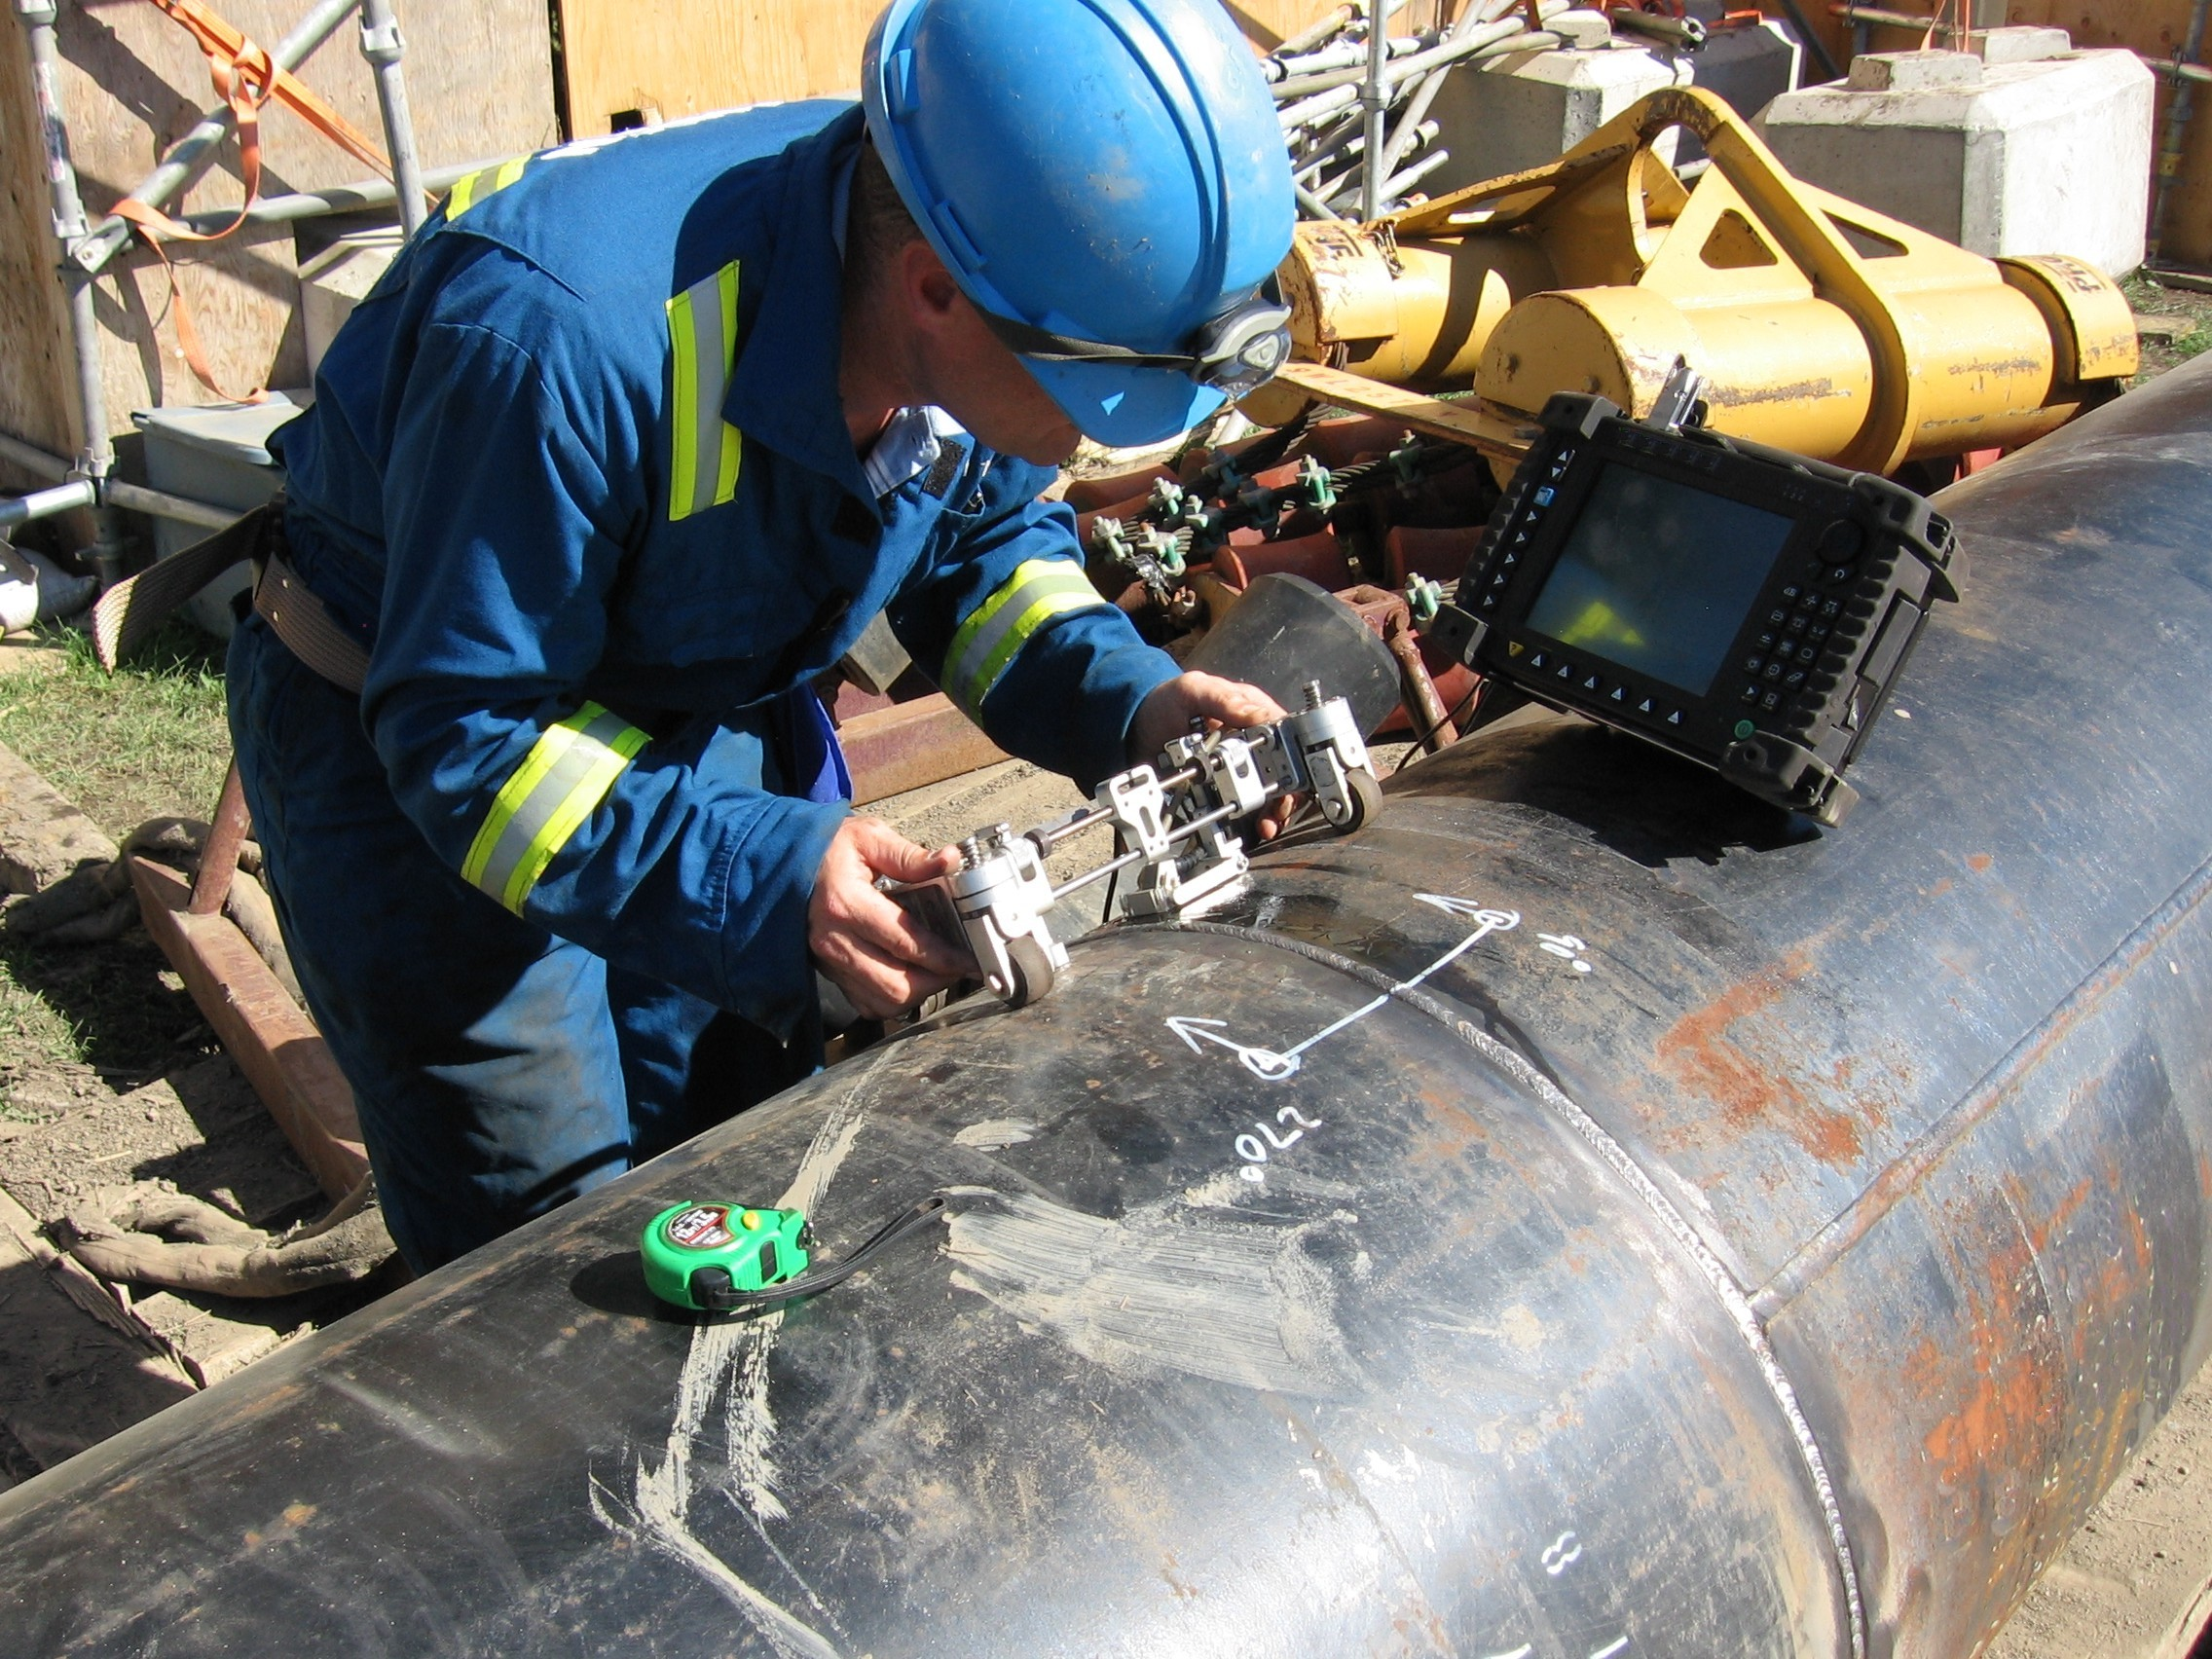
\includegraphics[height=3cm]{img/us_test.jpg}\\
				{\tiny{\raggedright \itshape Image Davidmack}\\ \centering \scriptsize{Contrôle sur pipeline}}
			\end{figure}		
			\column{0.5\textwidth}
			\begin{figure}
				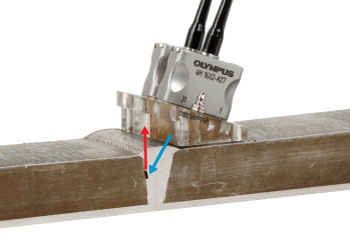
\includegraphics[height=3cm]{img/olympus.jpg}\\
				 {\tiny{\itshape Image Olympus}\\ \centering			\scriptsize{Exemple de test en réflexion}}
			\end{figure}
		\end{columns}	
		\vspace{0.4cm}	

	%\begin{columns}
			%\column{.5\textwidth}
			Contrôle et évaluation de soudures :\\
			\begin{itemize}
				\item de centrales nucléaires (système de refroidissement)
				\item de pipelines 
			\end{itemize}
			%\column{.05\textwidth}
			%\ding{222}
			%\column{.45\textwidth}
			%\centering
			\vspace{-0.4cm}
			\begin{columns}
			\column{0.7\textwidth}
			\centering
 			\indent \ding{222} porosité, fissure, manque de fusion, corrosion, corps étrangers,\ldots
 			\column{0.3\textwidth}
 			\centering
 			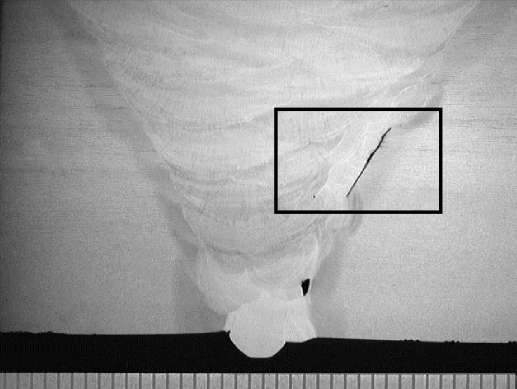
\includegraphics[width=0.95\textwidth]{img/defaut_soudure.png}\\
 			{\itshape \tiny Image extraite de Consonni et al., \\[-0.2cm]Insight, 2011}
 			\end{columns}
	%\end{columns}
\end{frame}


\subsection*{}
\begin{frame}{\insertsectionhead}
\begin{small}
\vspace{-0.5cm}
\hspace{1cm}
\onslide<2->{
\begin{picture}(0,0)(0,0)\put(50,5){
		\textcolor{red}{Forte anisotropie imprévisible}
}\end{picture}
}
	\begin{columns}[c]
			\column{.5\textwidth}<1->
			\centering
			\begin{figure}
				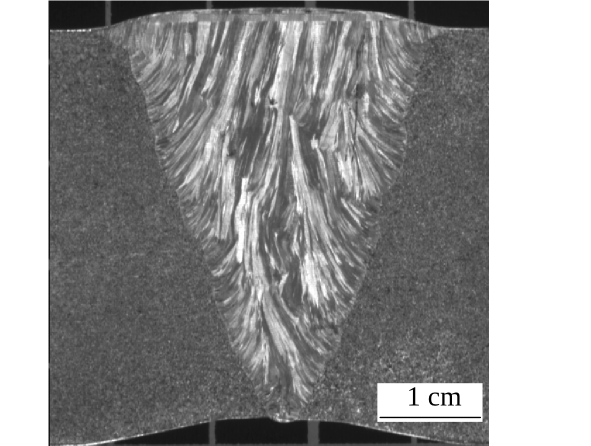
\includegraphics[height=2.7cm]{./img/soudure1.png}\\
				{\tiny{ \itshape Image extraite de Chassignole, 2010} \\ \centering \scriptsize Macrographie d'une soudure austénitique  }
			\end{figure}
			\column{.001\textwidth}<2->
			\hspace{-2.8cm}
			\vspace{2.5cm}
			\begin{tikzpicture}
					\draw[<-, thick,shorten <=2pt,shorten >=2pt,red] (-1.5,3)--(0.0,4.6);
			\end{tikzpicture}
			\column{.9\textwidth}<2->
			%\vfill
			\hspace{-1cm}
			$\hookrightarrow$ déviation et division du faisceau ultrasonore\\[0.2cm]
			\hspace{-0.5cm}
			\hspace{1cm}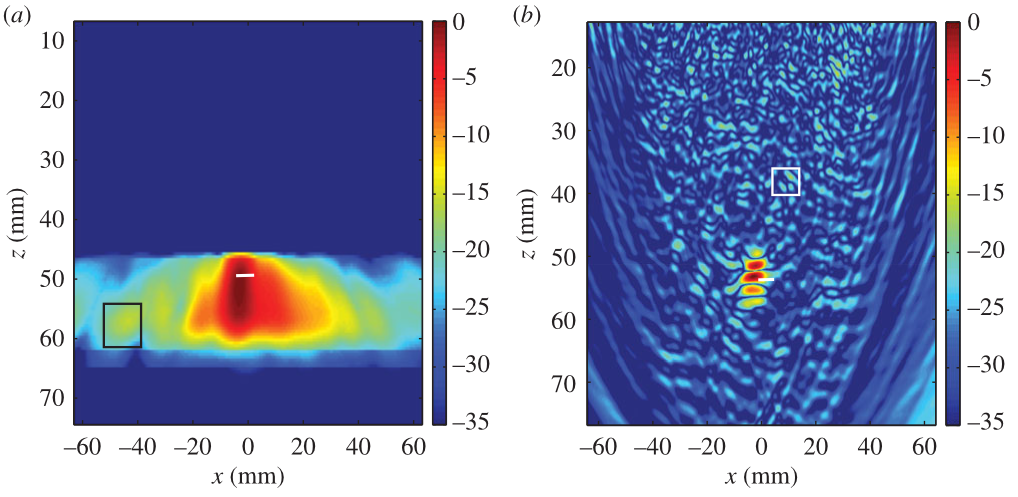
\includegraphics[height=2.5cm]{img/tfm_dort.png}\\
			{\tiny{ \itshape Images extraites de Cunningham et al., Proc. R. Soc., 2016} \\[0.2cm] \hspace{1cm} \scriptsize Méthodes DORT (gauche) et FTP (droite)\\[-0.1cm] \hspace{1.5cm}sur modèle EF de soudure anisotrope }
				
	\end{columns}
	%\vspace{0.3cm}
	\begin{columns}[c]
			\column{.5\textwidth}<1->
			%\begin{block}{}
				\begin{itemize}
					\item[$\bullet$] méthodes par sommation cohérente des signaux (ex : FTP)
					\item[$\bullet$] Décomposition des matrices de covariance (ex : DORT)
				\end{itemize}
			%\end{block}
			\column{.05\textwidth}<2->
			\ding{222}
			\column{.5\textwidth}<2->
				\begin{itemize}
					\item[\ding{55}] requièrent une connaissance\\ \emph{a priori} de la vitesse\\
					\item[\ding{55}] sujettes aux artefacts
				\end{itemize}
	\end{columns}
	\vspace{0.1cm}
	\begin{columns}[c]
		\column{.5\textwidth}<3->
			\begin{itemize}
				\item[$\bullet$] Résolution d'un problème d'optimisation
			\end{itemize}
		\column{.05\textwidth}<3->
			\ding{222}
		\column{.5\textwidth}<3->
			\begin{itemize}
			\item optimisation topologique :\\\hspace{-0.5cm}\small{\emph{Dominguez et al.}, \emph{Rodriguez et al.}}\\[0.1cm]
			\item[\ding{51}] {reconstruction d'un ensemble de paramètres : FWI}
		\end{itemize}		
	\end{columns}
\end{small}
\end{frame} 


\section{La FWI}
\subsection*{}
\begin{frame}{La Full Waveform Inversion}
	\begin{columns}
		\column{0.6\textwidth}
		\begin{itemize}
			\item Développée pour la géophysique\\[0.3cm]
			\item Estimation des paramètres élastiques\\ $~~~~~~\hookrightarrow$ optimisation locale\\[0.3cm]
			\item Utilise tout le champ d'onde\\[0.3cm]
		\end{itemize}
		\column{0.5\textwidth}
		\begin{figure}
			\centering
			\hspace{-0.3cm}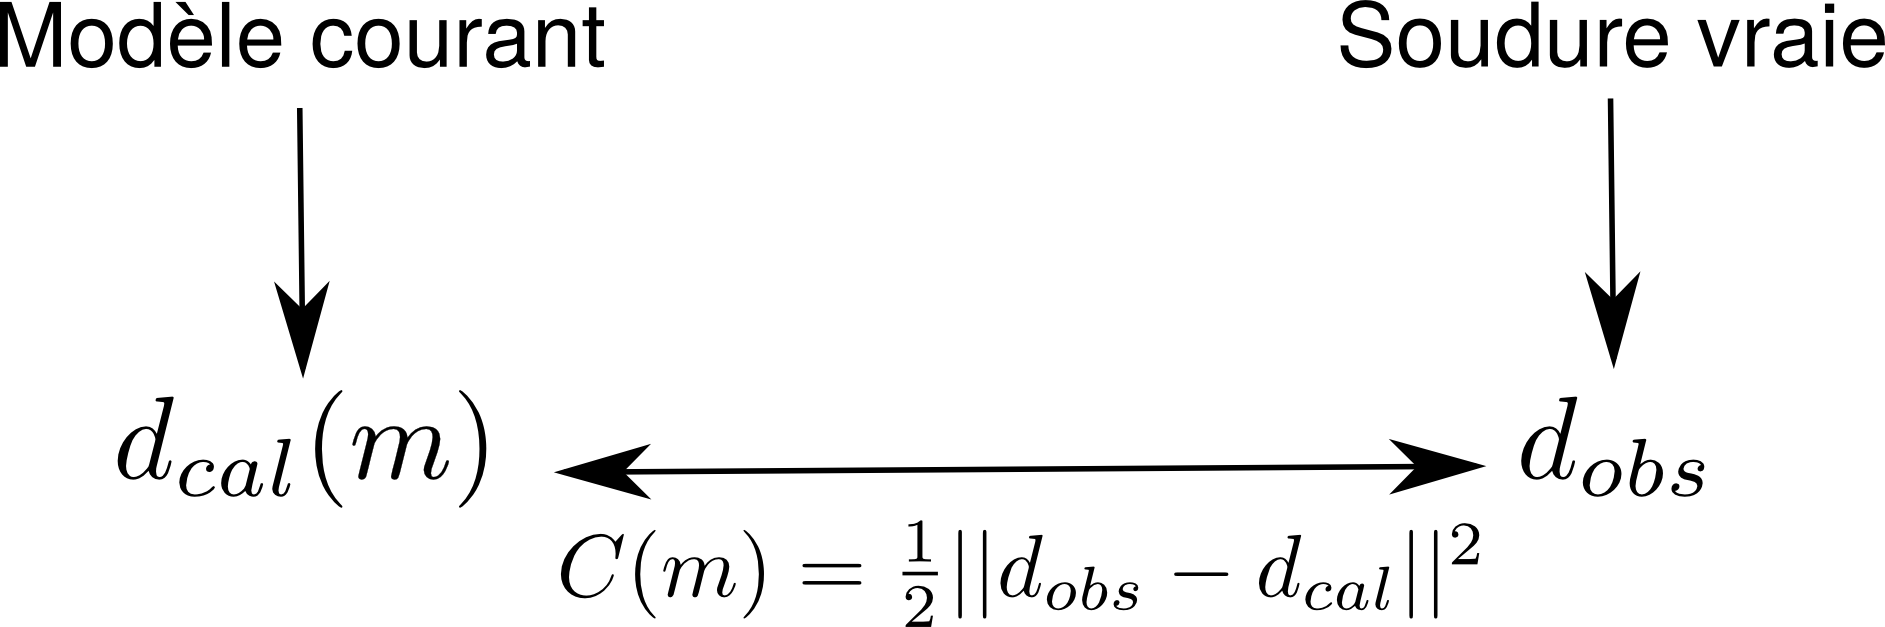
\includegraphics[width=\textwidth]{img/schema_fwi2.png}
		\end{figure}
	\end{columns}
	
\end{frame}

%\subsection*{}
%\begin{frame}{\insertsectionhead}
%	\vspace{-0.5cm}
%	\begin{figure}
%		\centering
%			\begin{tikzpicture}
		\node (init) [draw=black, align=center] at (0,0) {Paramètres initiaux \\ $\bm{m}_{0}$};
		\node (dir) [below=0.7cm of init , draw=black,align=center] {Problème direct :\\ éléments finis \\ ou différences finies};
		\path[->, thick,shorten <=2pt,shorten >=2pt] (init) edge (dir);
		\node (dcal) [draw=black, right=0.7cm of dir, align=center] {Données calculées \\ $\bm{d}_{cal}(\bm{m})$};
		\path[->, thick,shorten <=2pt,shorten >=2pt] (dir) edge (dcal);
		\node (dobs) [draw=black, right=0.7cm of dcal, align=center] {Données de mesures \\ $\bm{d}_{obs}$};
		\node (fc) [draw=black,below right= 0.7cm and -2cm of dcal, align=center] {Fonction de coût \\ $C(\bm{m})=\frac{1}{2}||\bm{d}_{obs}-\bm{d}_{cal}(\bm{m})||^{2}$};
		%\draw[|-,-|,->, thick,] (dobs.south) |-+(0,-1em)-| (fc.north);
		%\draw[|-,-|,-> thick,] (dcal.south) |-+(0,-1em)-| (fc.north);
		\path[->, thick,shorten <=2pt,shorten >=2pt] (dcal) edge (fc);
		\path[->, thick,shorten <=2pt,shorten >=2pt] (dobs) edge (fc);
		\path[->, thick,shorten <=2pt,shorten >=2pt] (dir) edge (dcal);
		\node (m) [draw=black, below left=0.7cm and -6cm of fc, align=center] {Problème inverse : \\~\\ 
			\begin{minipage}{0.35\textwidth}
				\centering
				Calcul du gradient $C'(\bm{m})$
				Calcul du hessien $C''(\bm{m})$
			\end{minipage}
			\vline
			\begin{minipage}{0.3\textwidth}
				\centering
				~$\bm{\Delta m}=-(C'')^{-1}C'$
			\end{minipage}
			\vline
			\begin{minipage}{0.35\textwidth}
				\centering
				Mise à jour du modèle : \\ $\bm{m} := \bm{m}+ \bm{\Delta m}$
			\end{minipage}
		};
		\path[->, thick,shorten <=2pt,shorten >=2pt] (fc) edge (m);
		\path[->, thick,shorten <=2pt,shorten >=2pt] (m) edge (dir);		
	\end{tikzpicture}
%	\end{figure}
%\end{frame}


\section{Résolution de la FWI}
%\subsection*{}
%\begin{frame}{\insertsectionhead}
%	\begin{itemize}
%		\item<1-> Fonction de coût : $C(\bm{m})=\frac{1}{2}||\bm{d}_{obs}-\bm{d}_{cal}(\bm{m})||^{2}$ \\[0.5cm]
%		\item \only<1-1>{Perturbation du modèle : $\bm{\Delta m}=-(C'')^{-1}$\fcolorbox{white!0}{white!0}{$C'$}} \onslide<2->{Perturbation du modèle : $\bm{\Delta m}=-(C'')^{-1}$\fcolorbox{DeepSkyBlue4}{white!0}{$C'$}}
%	\end{itemize}
%	\onslide<2-> {
%		\begin{figure}
%			\vspace{-0.84cm}\hspace{2.8cm}\begin{tikzpicture}	
%					\node (grad) at (10,0) {};
%					\node (exp) at ($(grad)+(-1.5,-1.1)$) {};
%					\draw[->, thick,shorten <=2pt,shorten >=2pt,DeepSkyBlue4] (grad) -- (exp);		
%				\end{tikzpicture}
%		\end{figure}
%	
%	
%%	\only<2-2>{
%%		\vspace{-0.8cm}\begin{equation}
%%			\frac{\partial C}{\partial m_{i}}= \tr{\tilde{\bm{d}}_{cal}} \tr{\left( \frac{\partial\bm{A}}{\partial m_{i}} \right)}\bm{A}^{-1} (\tilde{\bm{d}}_{obs} - \tilde{\bm{d}}_{cal}) 
%%		\end{equation}
%%	}
%
%		\vspace{-0.8cm}\begin{equation}
%			\frac{\partial C}{\partial m_{i}}= \tr{\tilde{\bm{d}}_{cal}} \tr{\left( \frac{\partial\bm{A}}{\partial m_{i}} \right)} \textcolor{DeepSkyBlue4}{\underbrace{\textcolor{black}{\bm{A}^{-1} (\tilde{\bm{d}}_{obs} - \tilde{\bm{d}}_{cal})}}_{\text{résidus rétropopagés}}}
%		\end{equation}
%
%			~\\$\bm{A}$ : opérateur équation d'onde (élastique ou acoustique)
%	}
%\end{frame}


\subsection*{}
\begin{frame}{\insertsectionhead}
	\only<1-3>{
		\begin{equation*}
			\frac{\partial C}{\partial m_{i}}= \textcolor{DeepSkyBlue4}{\underbrace{\textcolor{black}{\tr{\tilde{\bm{d}}_{cal}}}}_{\substack{\text{champ incident}}}}
			 \tr{\left( \frac{\partial\bm{A}}{\partial m_{i}} \right)} 
			 \textcolor{DeepSkyBlue4}{\underbrace{\textcolor{black}{\bm{\lambda}}}_{\substack{\text{résidus rétropopagés}}}}
		\end{equation*}
	}
	\only<4->{
		\vspace{-0.06cm}\begin{equation*}
			\frac{\partial C}{\partial m_{i}}= \textcolor{DeepSkyBlue4}{\underbrace{\textcolor{black}{\tr{\tilde{\bm{d}}_{cal}}}}_{\substack{\text{champ incident}}}}
			 \text{\fcolorbox{DeepSkyBlue4}{white!0}{$\tr{\left( \frac{\partial\bm{A}}{\partial m_{i}} \right)}$ }}
			 \textcolor{DeepSkyBlue4}{\underbrace{\textcolor{black}{\bm{\lambda}}}_{\substack{\text{résidus rétropopagés}}}}
		\end{equation*}		
%	\begin{picture}(0,0)(0,0)\put(155,-105){
%		\begin{tikzpicture}	
%					\node (A) at (6,0) {};
%					\node (ray) at ($(A)+(0,-4)$) {};
%					\draw[->, thick,shorten <=2pt,shorten >=2pt,DeepSkyBlue4] (A) -- (ray);		
%		\end{tikzpicture}
%	}\end{picture}
	}
	\begin{equation*}
		~~~~~~~~\sim~ \Re\left( e^{j k_{0} \bm{s.x}} \right)~~~~~~~~~\sim~ \Re\left( e^{j k_{0} \bm{r.x}} \right)
	\end{equation*}
		
	\onslide<2->{
		\begin{itemize}
			\item Résolution du gradient :\vspace{-0.34cm}
			\begin{align}
				k=|\bm{s}+\bm{r}|=&\frac{\omega}{c}2\cos\left( \frac{\theta}{2} \right)~~~~~~~~\\
				\hookrightarrow \text{~ maximale ($\lambda$/2) en HF et pour}~&\theta=0 \nonumber
			\end{align}	\vspace{-1cm}		
	}
		\only<1-3>{
			\begin{columns}
				\column{0.4\textwidth}<1-3>
				\begin{figure}
					\centering
					\vfill
					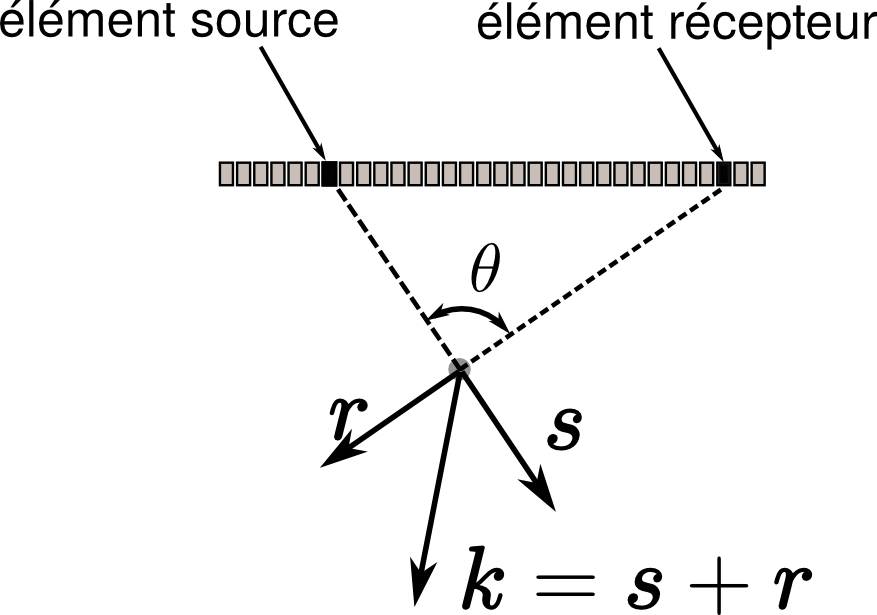
\includegraphics[height=2.5cm]{img/reso.png}	
				\end{figure}
				\column{0.55\textwidth}<3-3>
				\begin{figure}
					\centering
					\vspace{0.4cm} 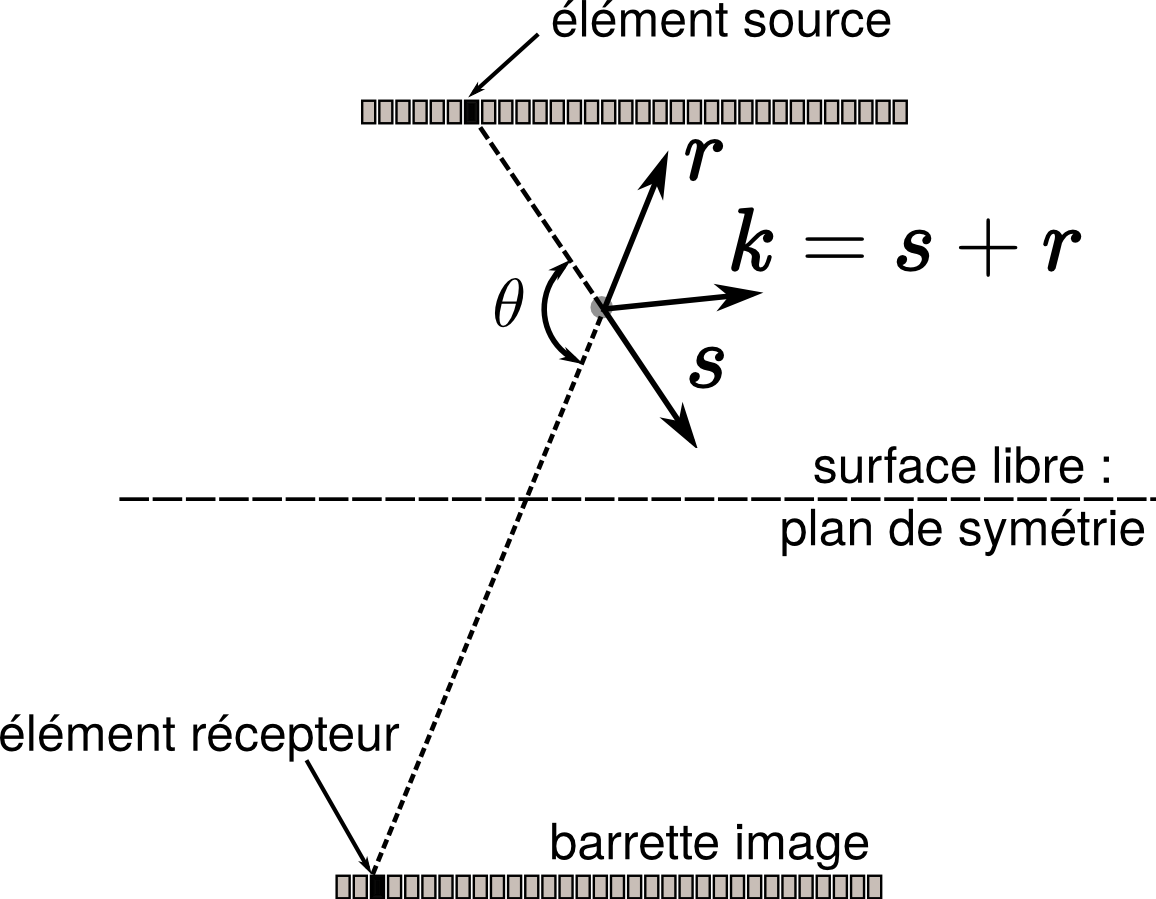
\includegraphics[height=3.7cm]{img/reso_surf_libre.png}
				\end{figure}		
			\end{columns}
		}
	

	\only<4->{		
		\vspace{0.7cm}\item Rayonnement des paramètres :\\[0.2cm] 
		\begin{figure}
			\hspace{-1cm}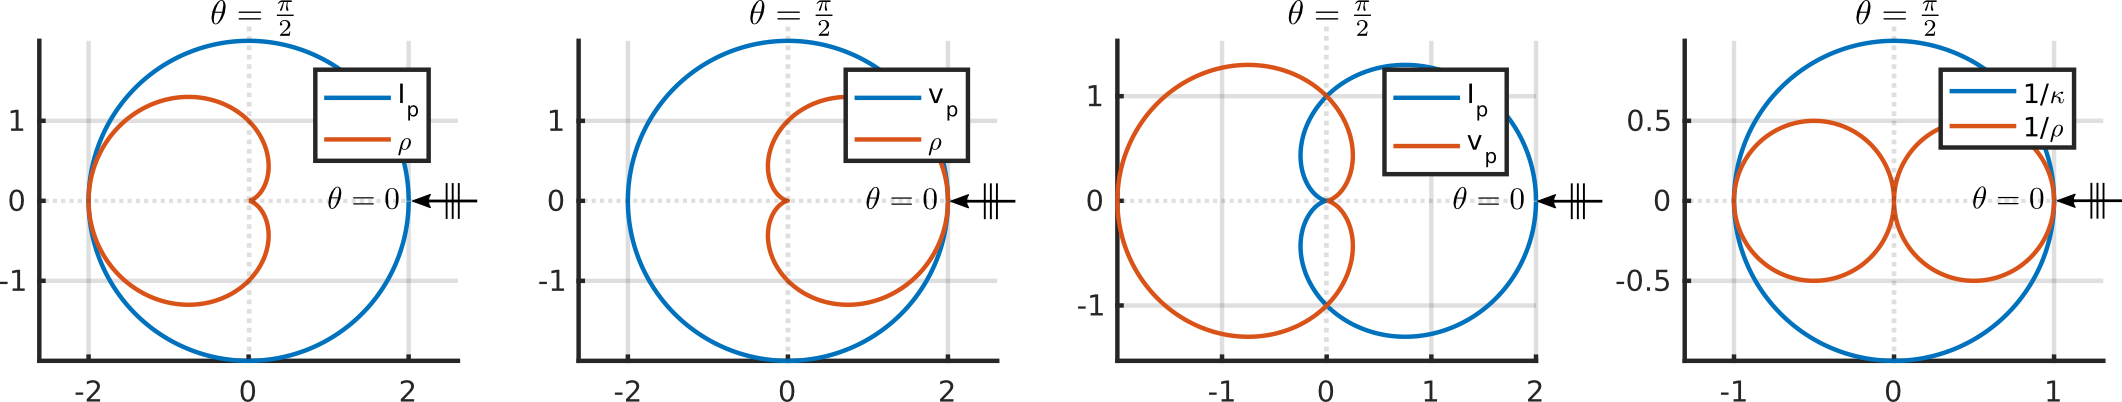
\includegraphics[height=2cm]{img/rayonnement.png}
		\end{figure}		
	}

	\end{itemize}
	\vspace{1cm}
\end{frame}

\section{Inversions en milieu isotrope}
\subsection*{}
\begin{frame}{\insertsectionhead}
	\begin{itemize}
		\item<1-> Milieu 2D, isotrope, acoustique
		\item<1-> Paramétrisation : vitesse + masse volumique
		\item<2-> Excitation : Ricker centré à 2 MHz 
	\end{itemize}	
	\only<1-1>{
	\begin{columns}
		\column{0.5\textwidth}
		\begin{figure}
			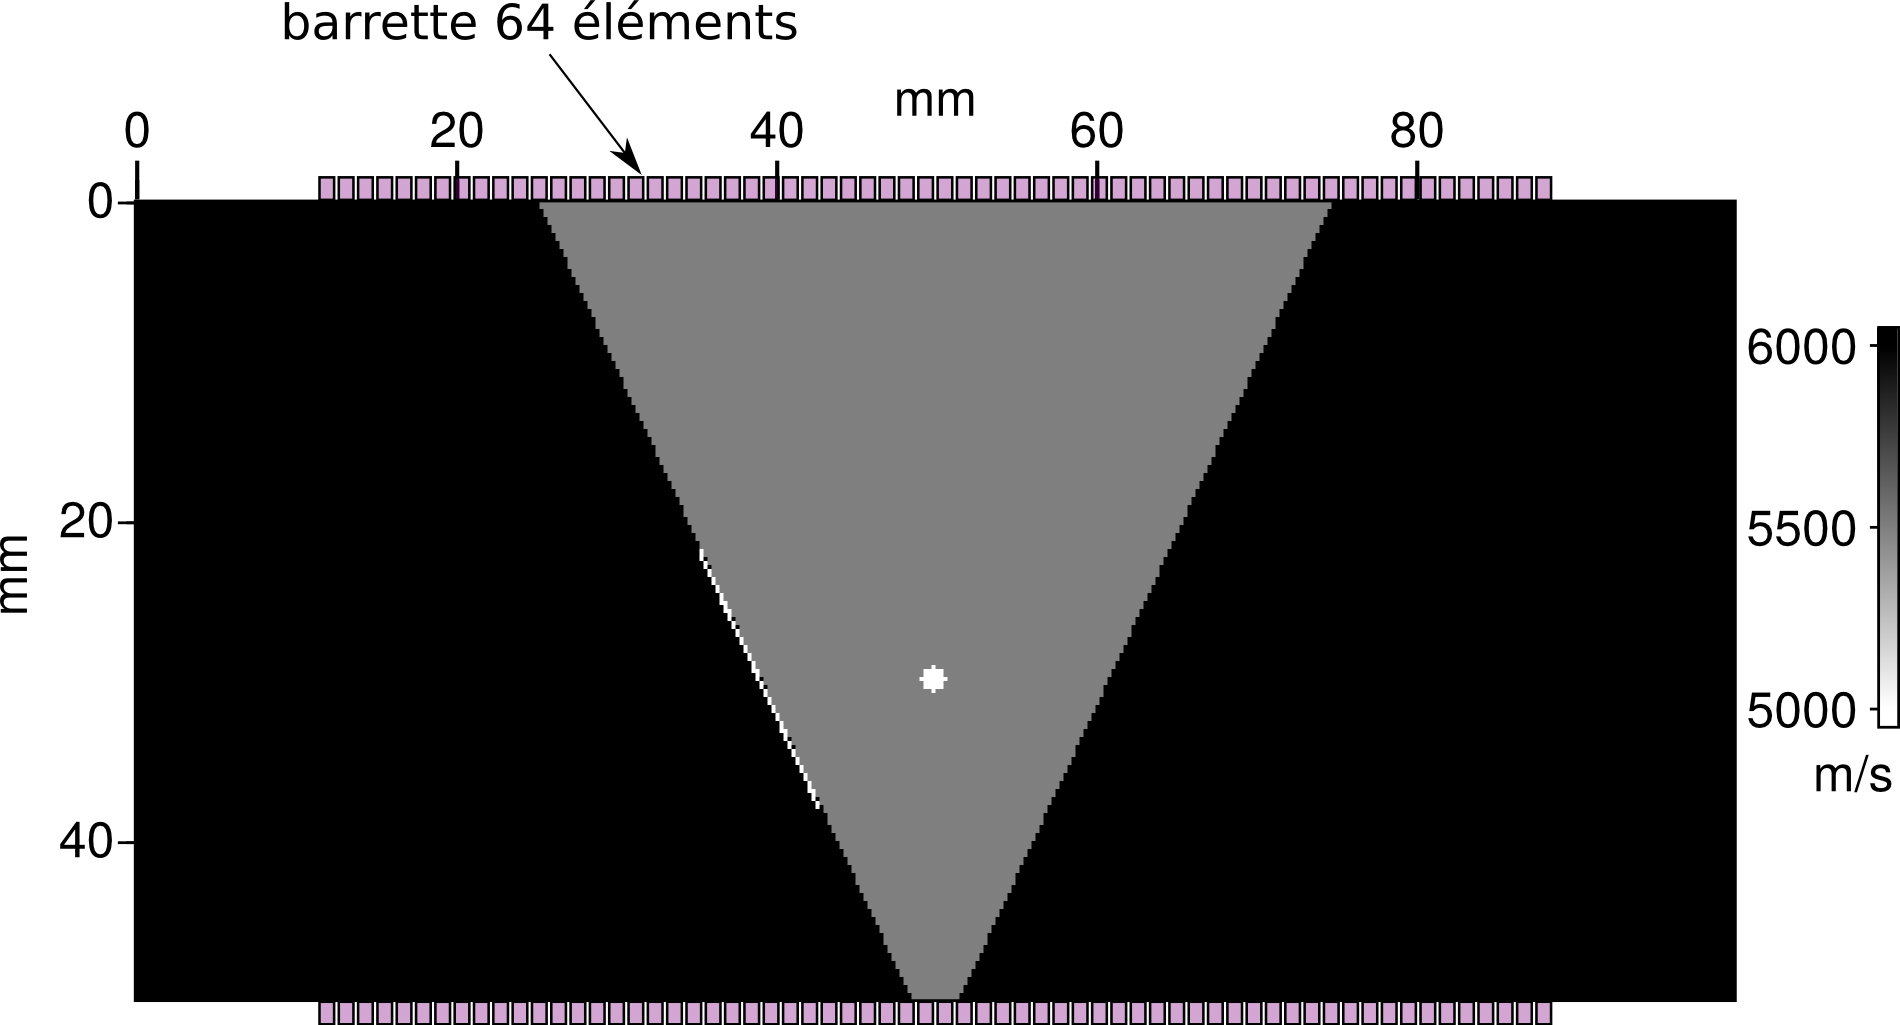
\includegraphics[width=\textwidth]{img/vp_true.png}\\
			{\small Vitesse vraie}
		\end{figure}
		\column{0.5\textwidth}
		\begin{figure}
			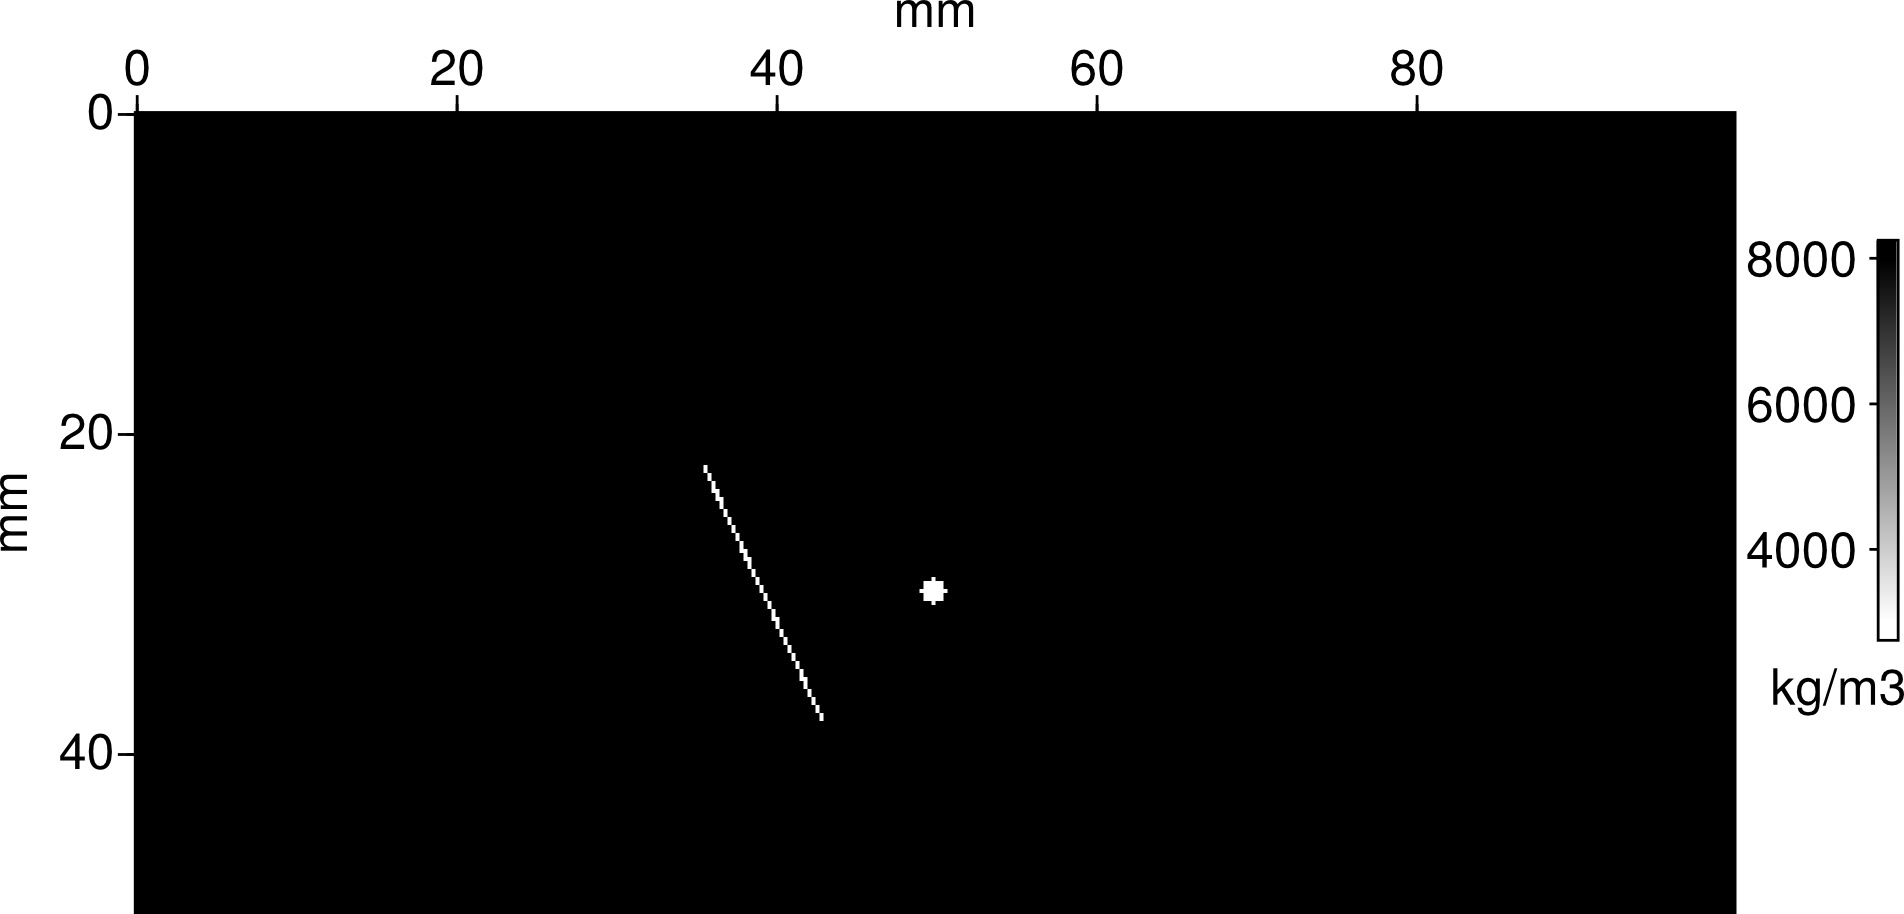
\includegraphics[width=\textwidth]{img/rho_true.png}\\
			{\small Masse volumique vraie}
		\end{figure}
	\end{columns}
	}
	
	\only<2->{
	\begin{columns}
		\column{0.5\textwidth}
		\begin{figure}
			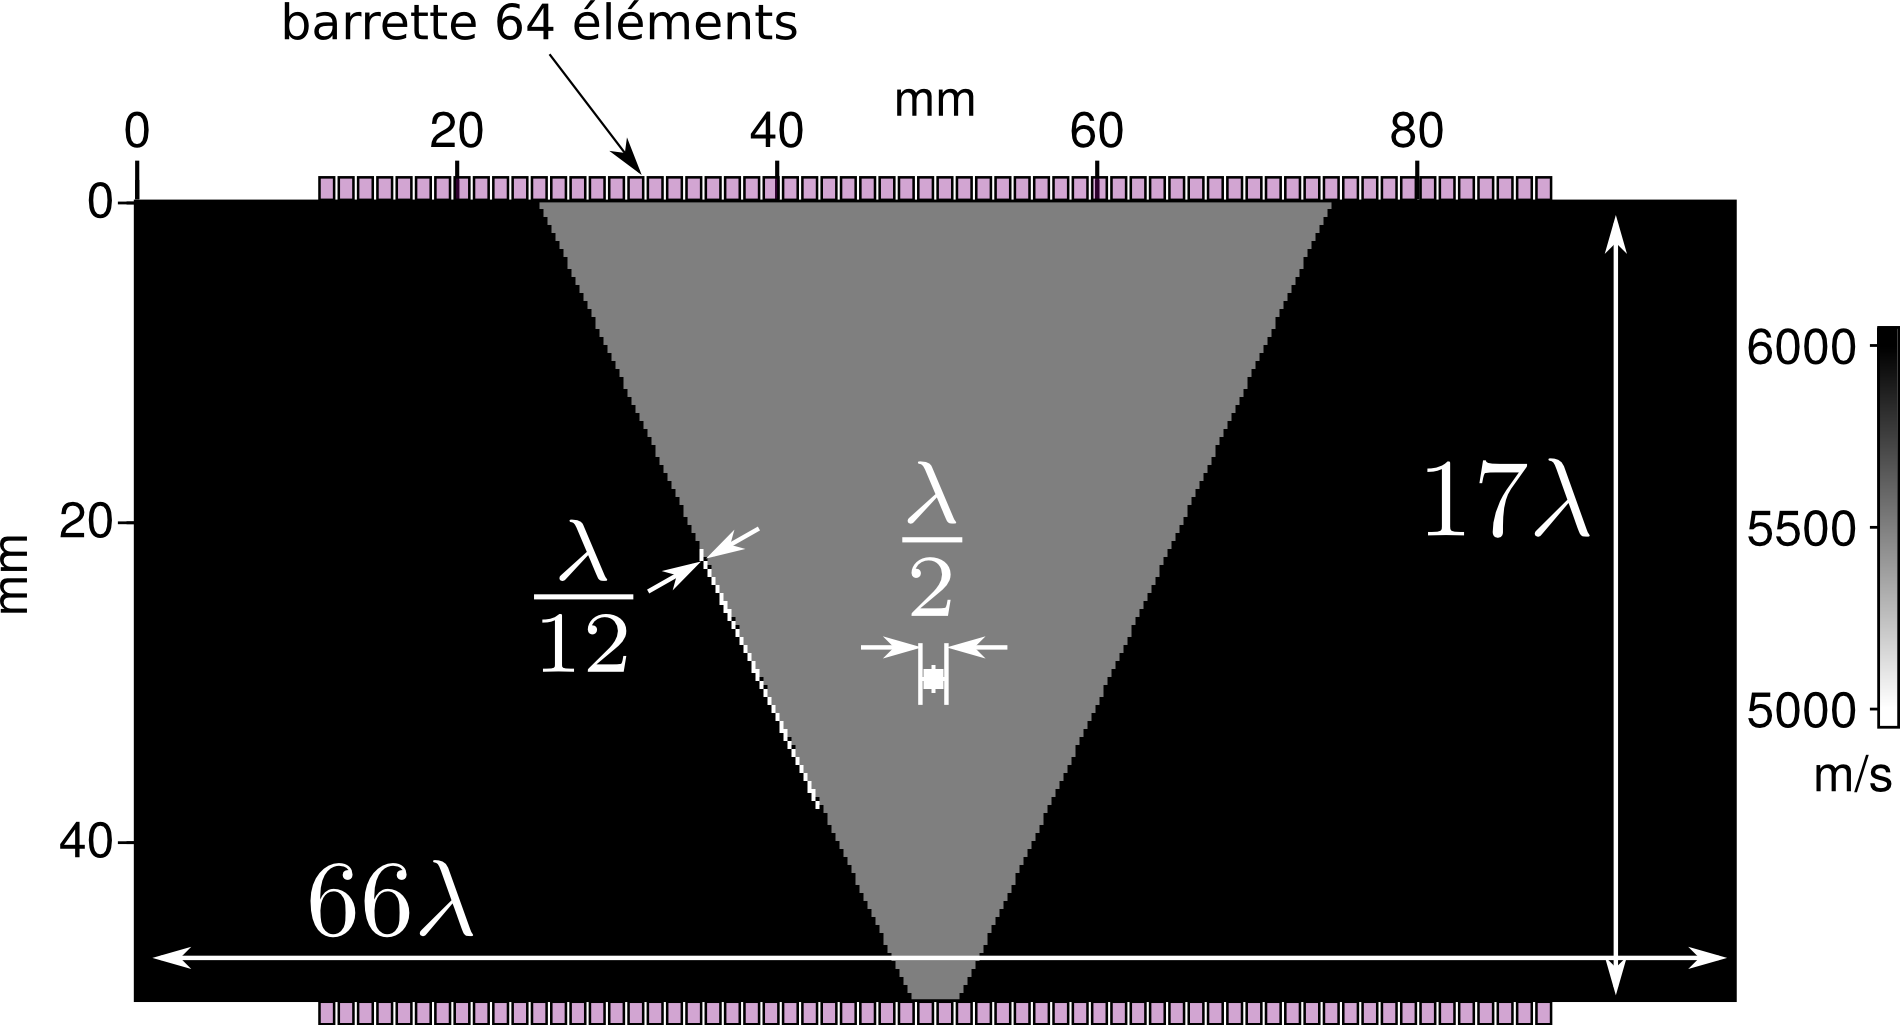
\includegraphics[width=\textwidth]{img/vp_true_lambda.png}\\
			{\small Vitesse vraie}
		\end{figure}
		\column{0.5\textwidth}
		\begin{figure}
			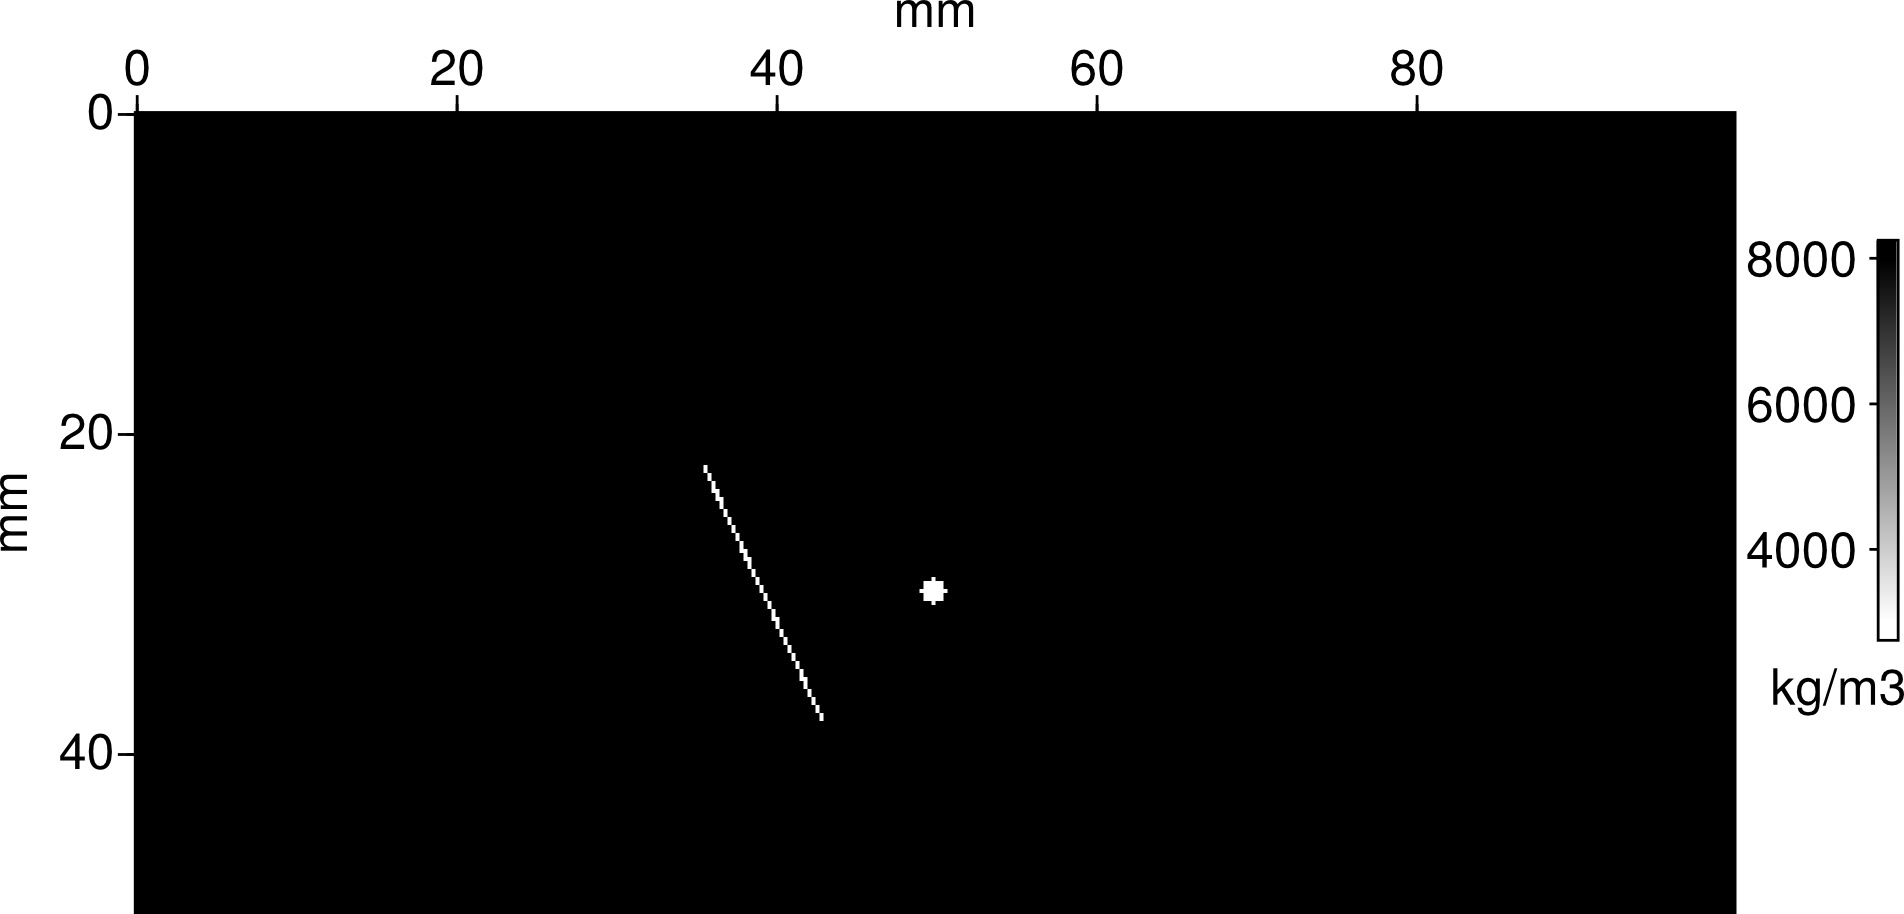
\includegraphics[width=\textwidth]{img/rho_true.png}\\
			{\small Masse volumique vraie}
		\end{figure}
	\end{columns}
	}
	
%	\vspace{1cm}
%	\begin{itemize}
%		\item 9 inversions successives de 200 kHz à 3 MHz pour
%			\begin{itemize}
%				\item mieux contraindre le problème
%				\item lever les ambiguïtés de déphasage 
%			\end{itemize}
%	\end{itemize}


\only<2->{
\begin{picture}(0,0)(0,0)\put(220,110){	
	\begin{tikzpicture}
			\node (a) at (0,0) {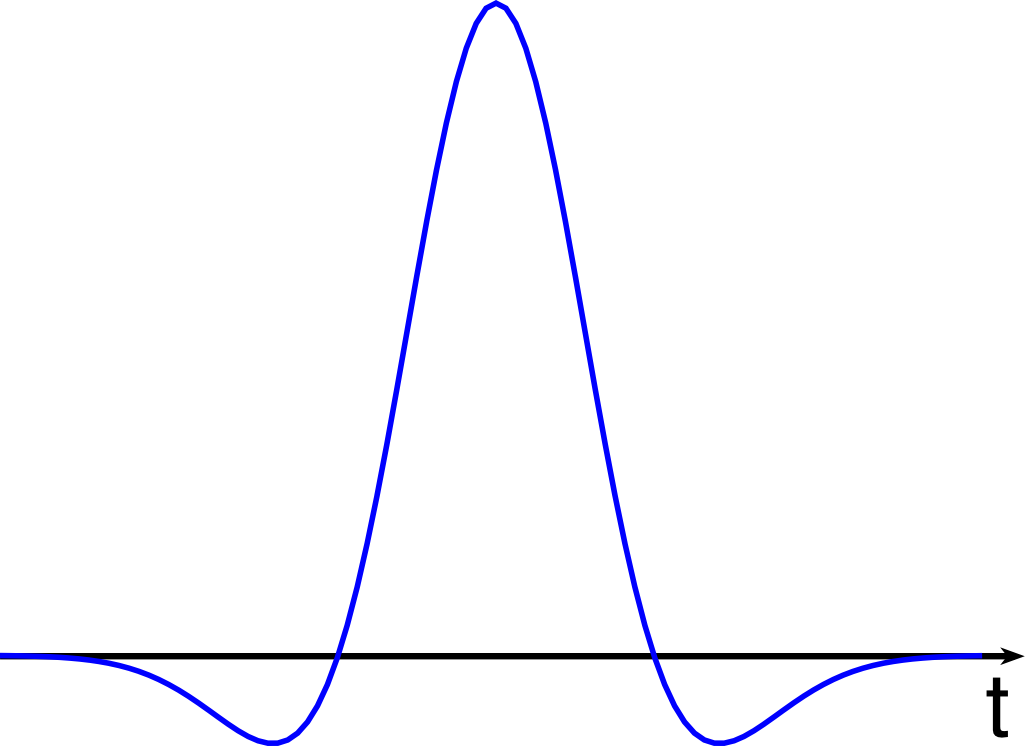
\includegraphics[height=1.5cm]{img/ricker.png}};
			\node (b) [below=-0cm of a] {\scriptsize Ondelette de Ricker};
	\end{tikzpicture}
}\end{picture}}


\end{frame}

\subsection{Stratégies d'inversion}
\begin{frame}{\insertsubsectionhead}
\begin{small}
	\begin{columns}
	\column{0.6\textwidth}
	\begin{itemize}
		\item pour mieux contraindre le problème
		\item pour lever les ambiguïtés de phase
	\end{itemize}
	\onslide<2->{2 critères hiérarchiques :}
	\begin{itemize}
		\item<2-> influence des paramètres sur les données %(cinématique, dynamique, prépondérance, ...) %Fort lissage de $\bm{\Delta m}$ : gaussien sur 2 $\lambda$
		\item<4-> contenu fréquentiel
	\end{itemize}
	\column{0.5\textwidth}
		\centering
		\vspace{-0.5cm}
		\only<3-4>{
		\includegraphics[height=2.7cm]{img/vp_smooth/vp_smooth.png}\\
		\scriptsize{~~}\\
		}
		\only<5-5>{
		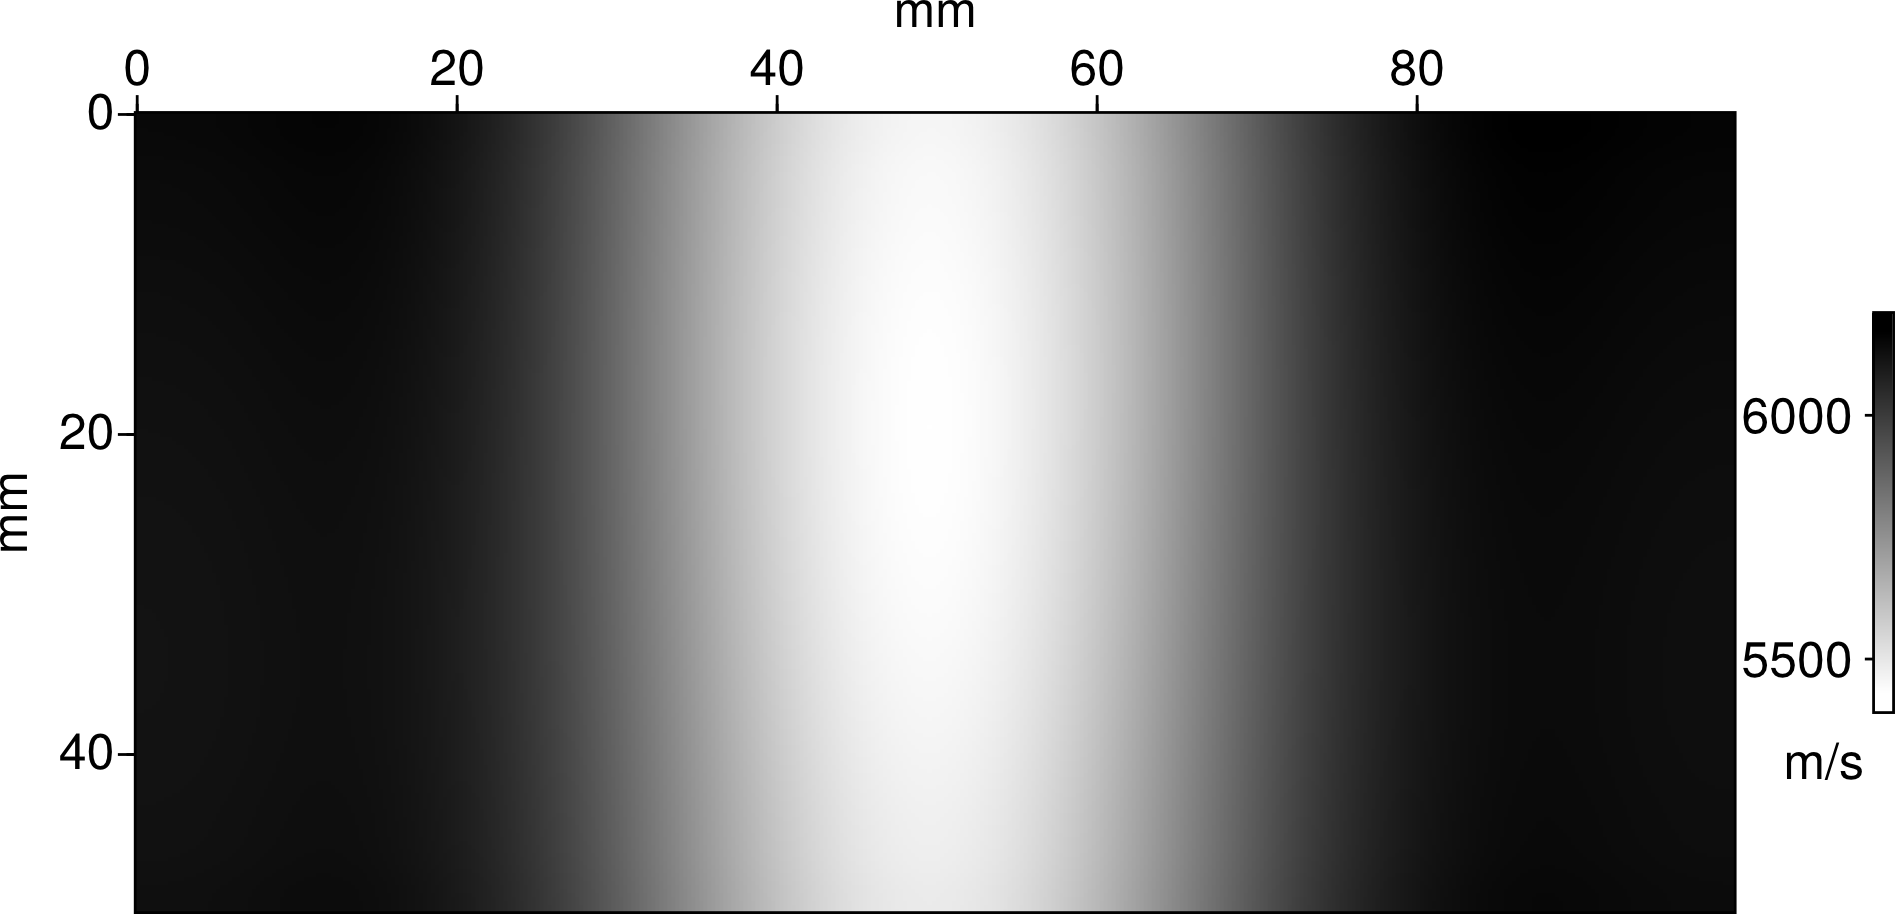
\includegraphics[height=2.7cm]{img/vp_smooth/vp_200k.png}\\
		\scriptsize{f$\sim$ 200 kHz}\\
		}
		\only<6-6>{
		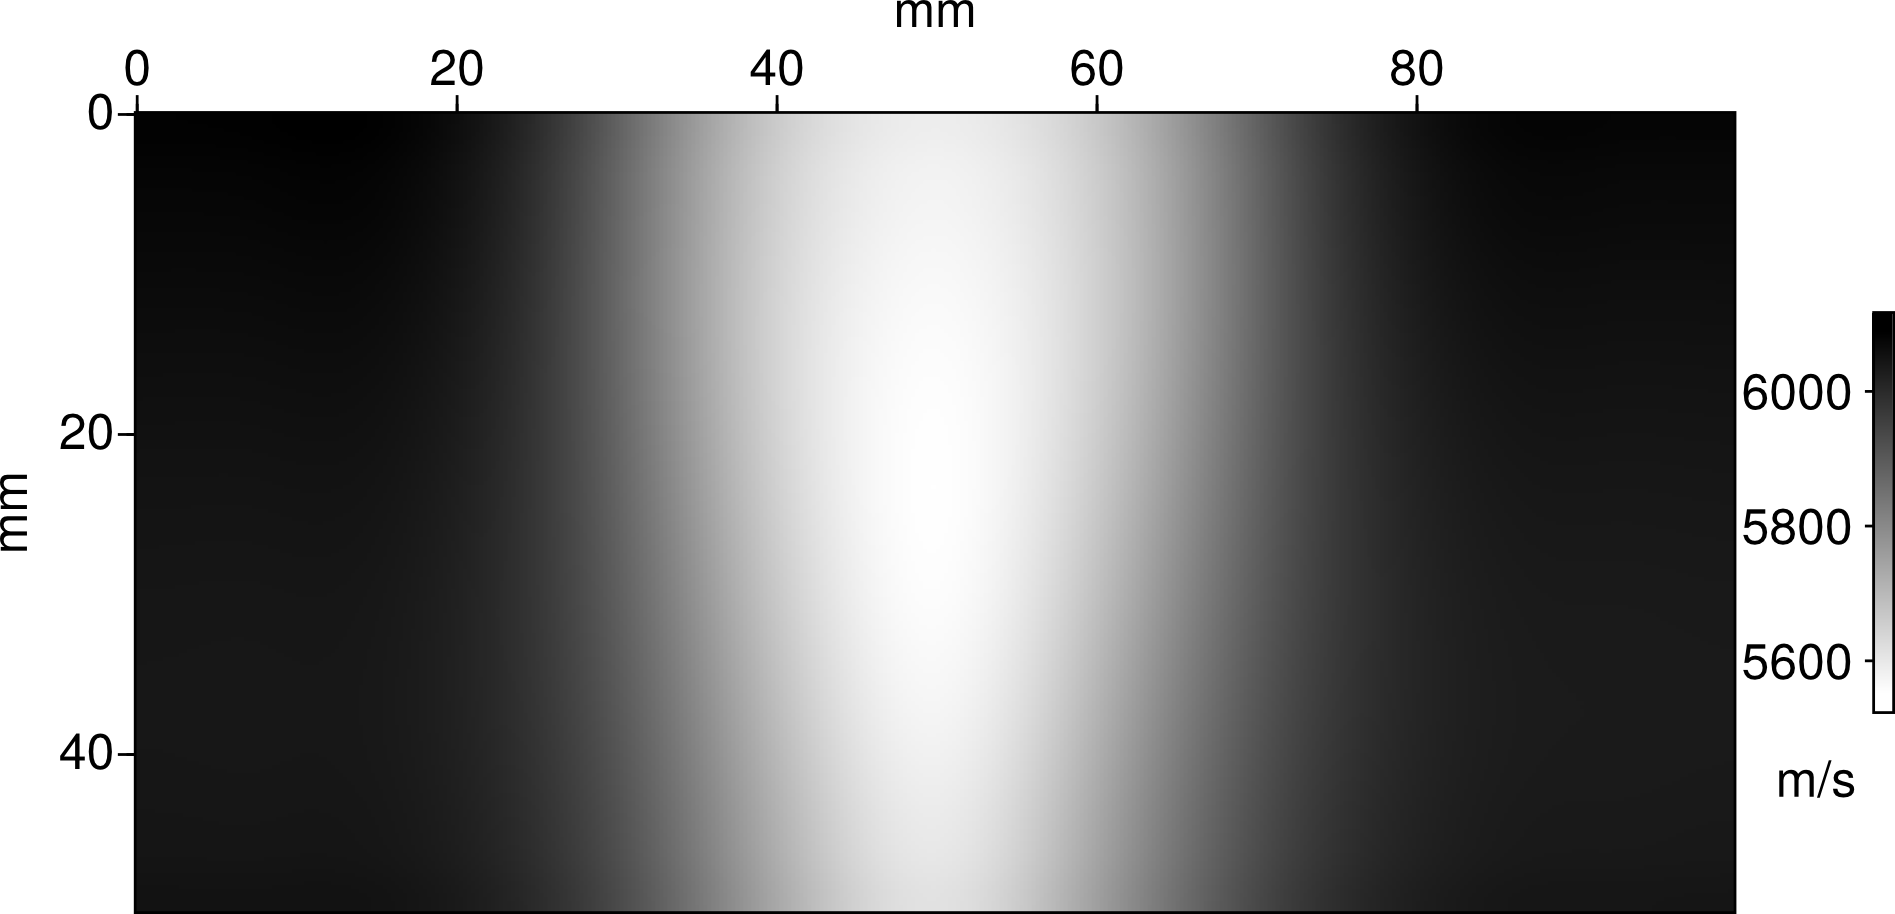
\includegraphics[height=2.7cm]{img/vp_smooth/vp_300k.png}\\
		\scriptsize{f$\sim$ 300 kHz}\\
		}	
		\only<7-7>{
		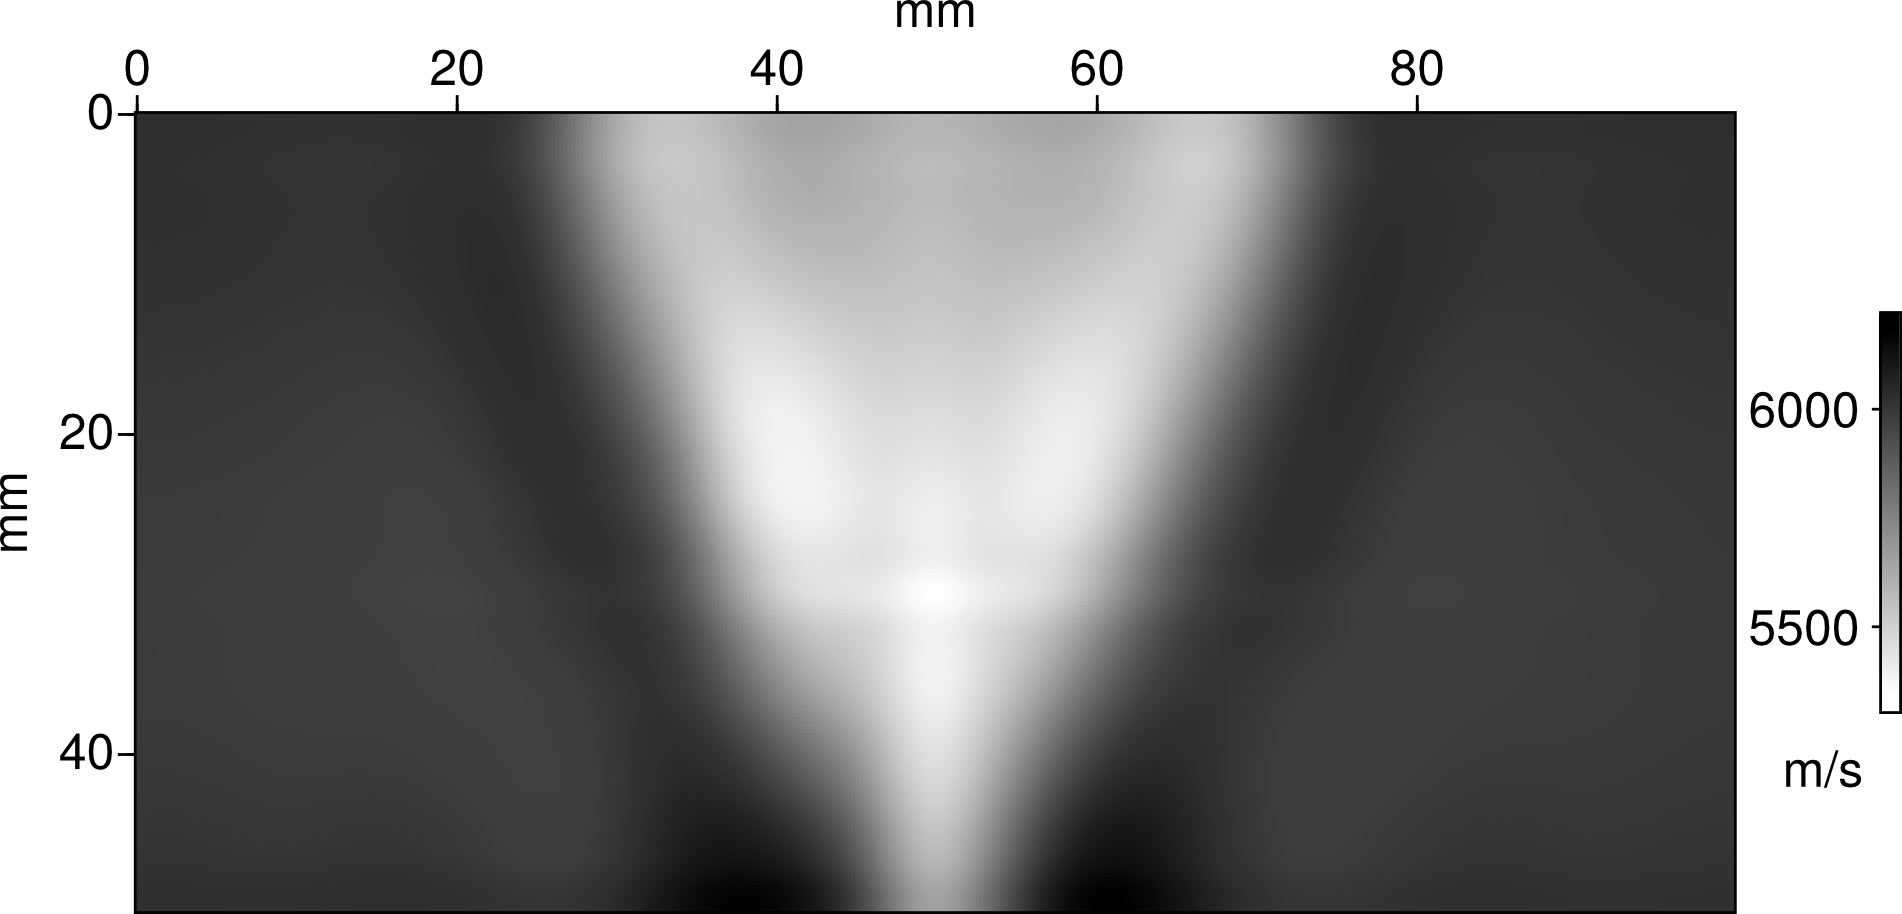
\includegraphics[height=2.7cm]{img/vp_smooth/vp_450k.png}\\
		\scriptsize{f$\sim$ 450 kHz}\\
		}
		\only<8-8>{
		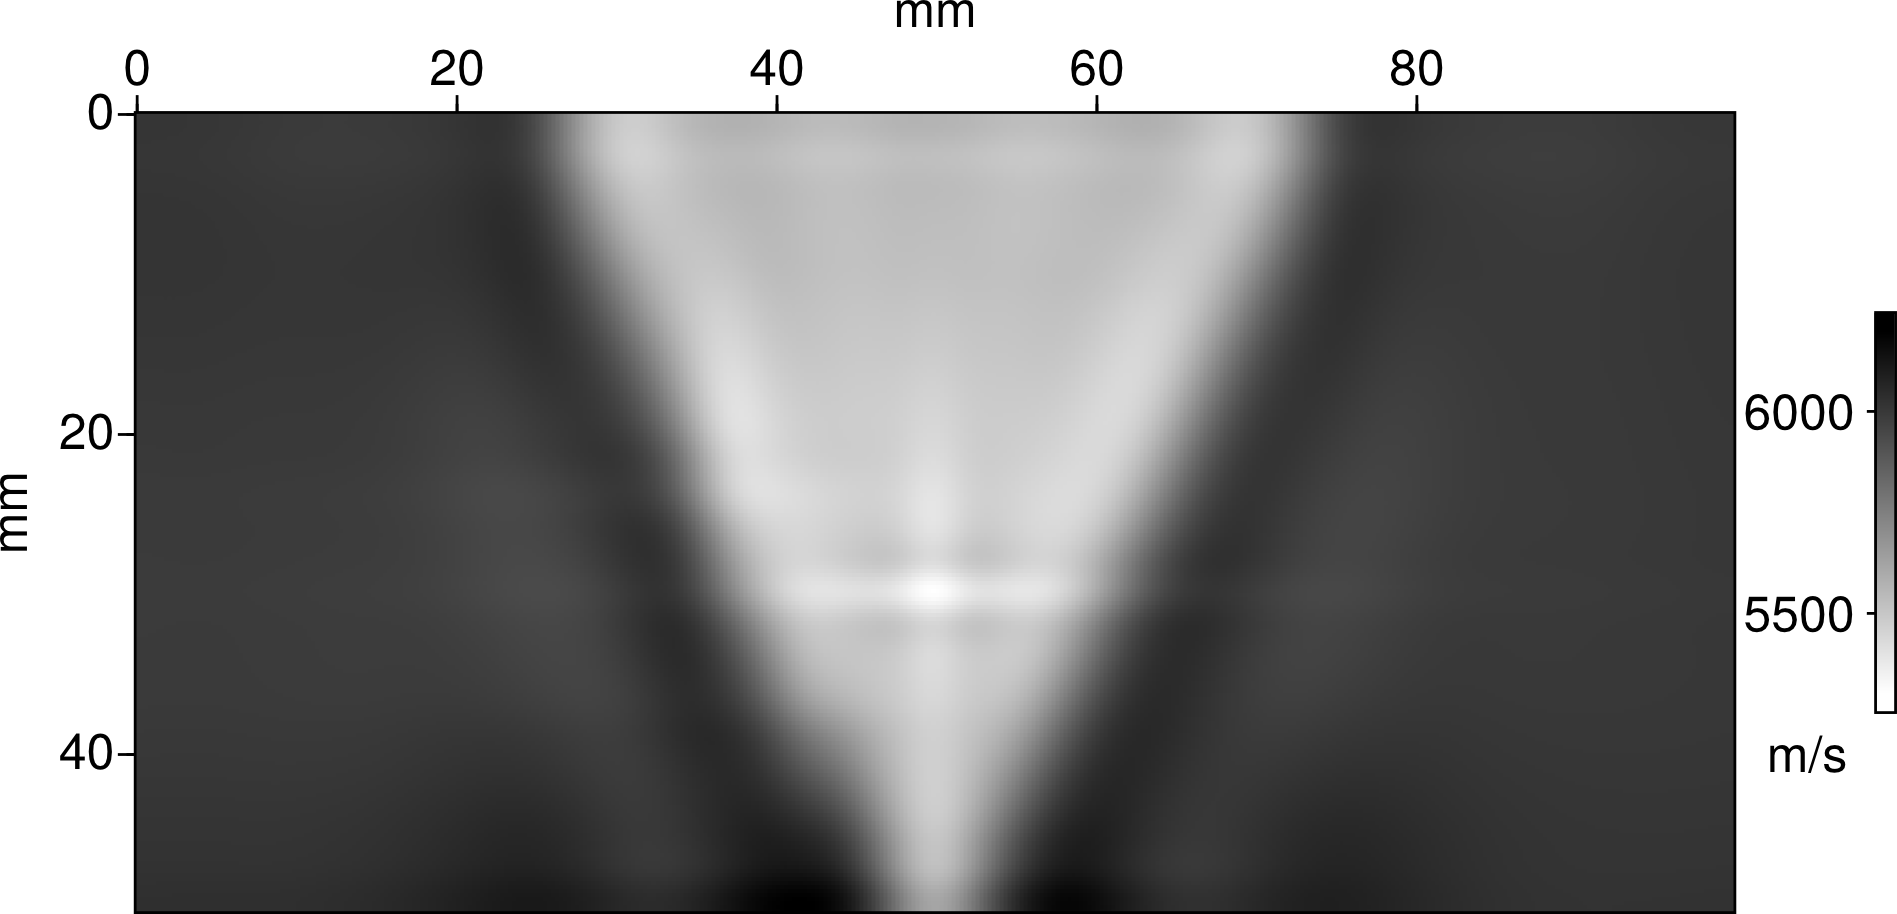
\includegraphics[height=2.7cm]{img/vp_smooth/vp_675k.png}\\
		\scriptsize{f$\sim$ 675 kHz}\\
		}
		\only<9-9>{
		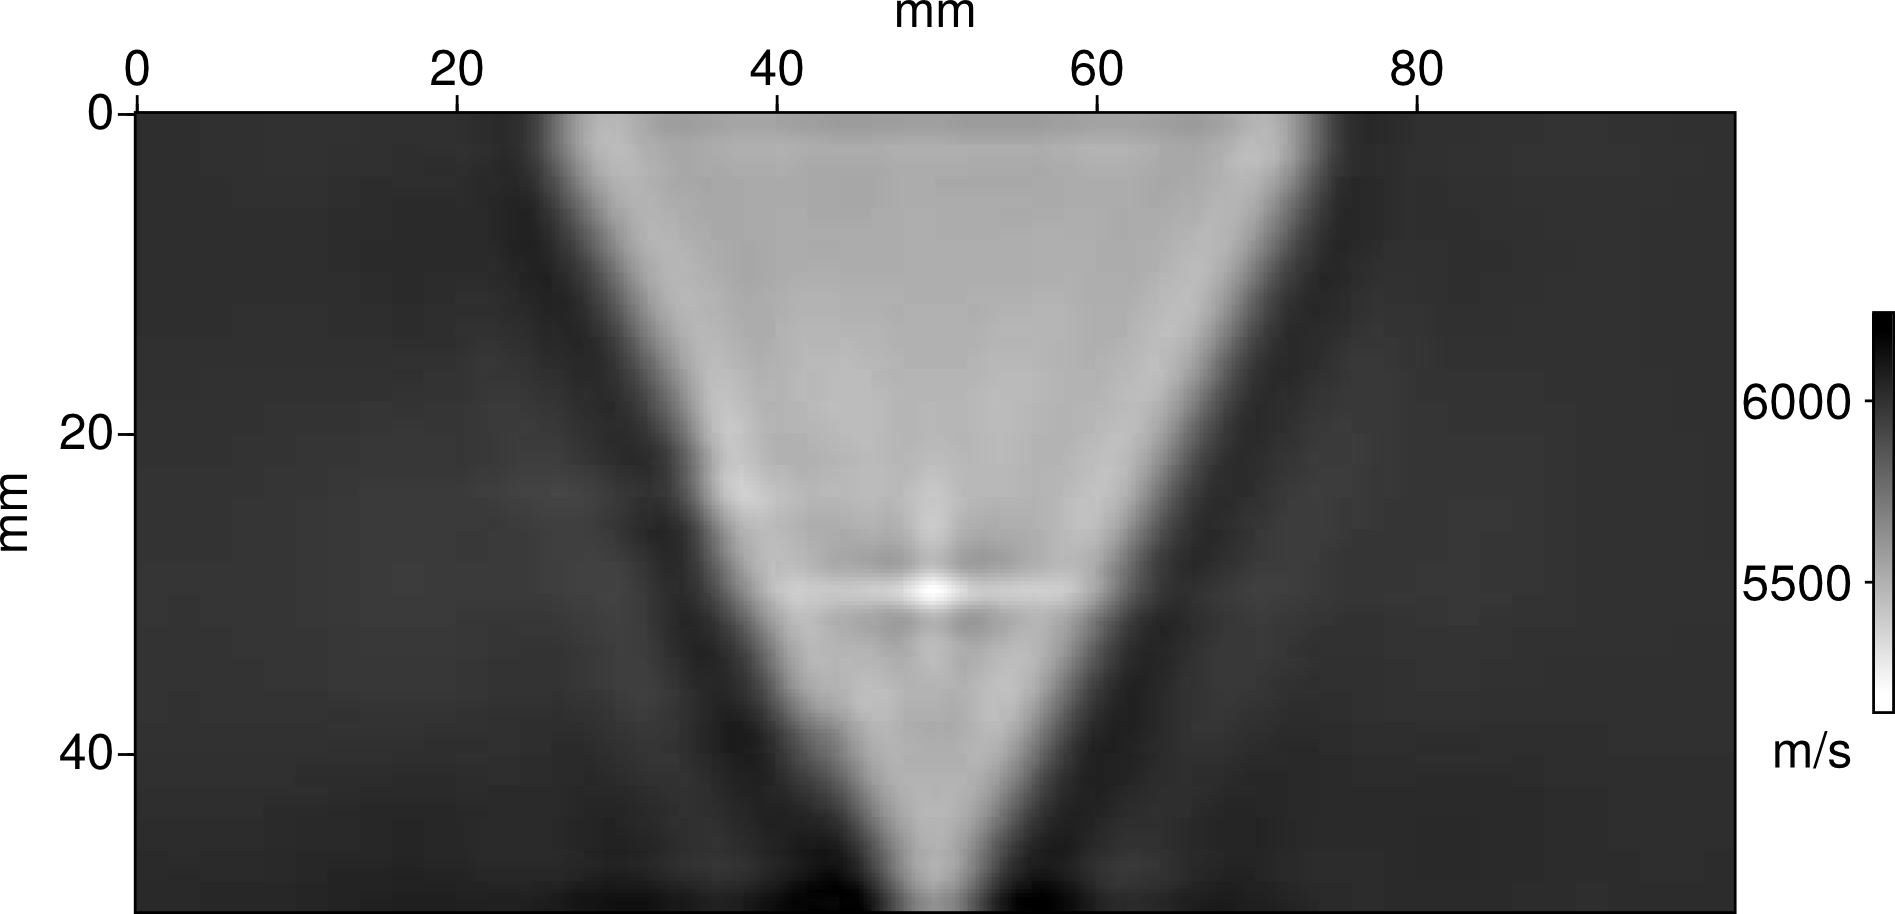
\includegraphics[height=2.7cm]{img/vp_smooth/vp_1000k.png}\\
		\scriptsize{f$\sim$ 1000 kHz}\\
		}
		\only<10-10>{
		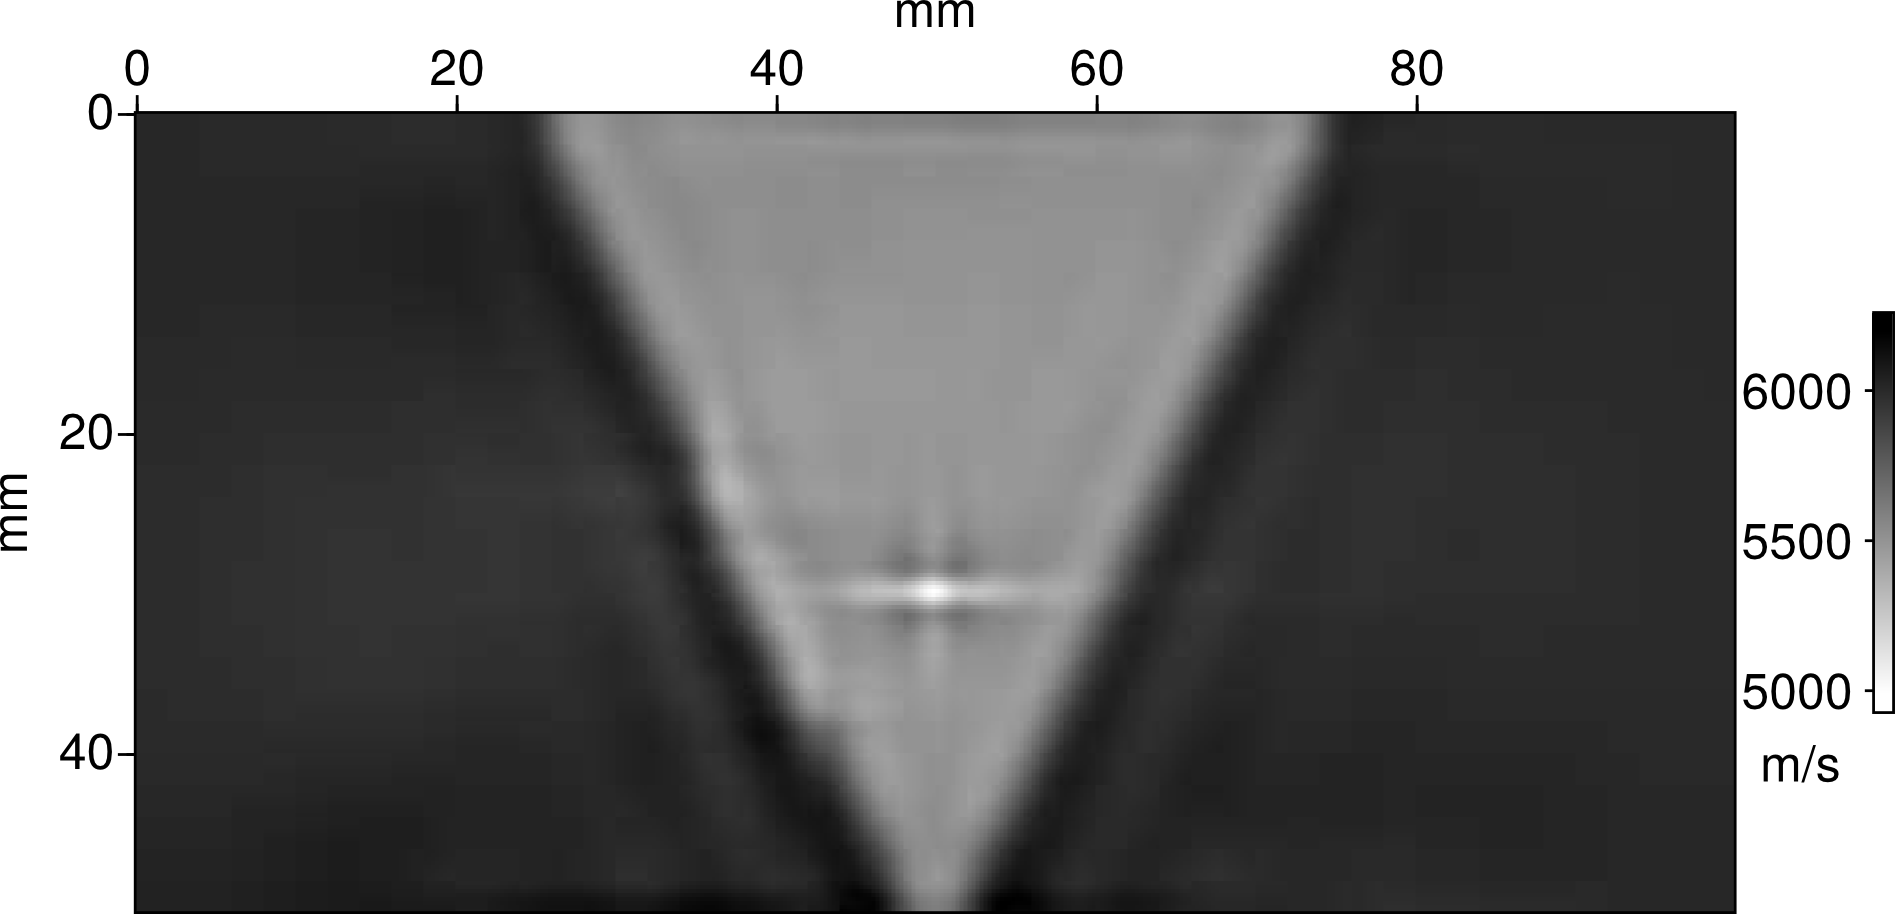
\includegraphics[height=2.7cm]{img/vp_smooth/vp_1500k.png}\\
		\scriptsize{f$\sim$ 1500 kHz}\\
		}
		\only<11->{
		\includegraphics[height=2.7cm]{img/vp_smooth/vp_smooth.png}\\
		\scriptsize{f$\sim$ 2200 kHz}\\
		}			
		\only<3->{\scriptsize{Construction d'un modèle de vitesse lissé}}
	\end{columns}
	\vspace{0.3cm}	
	\begin{columns}
		\column{0.3\textwidth}
		\onslide<2->{
		\centering
		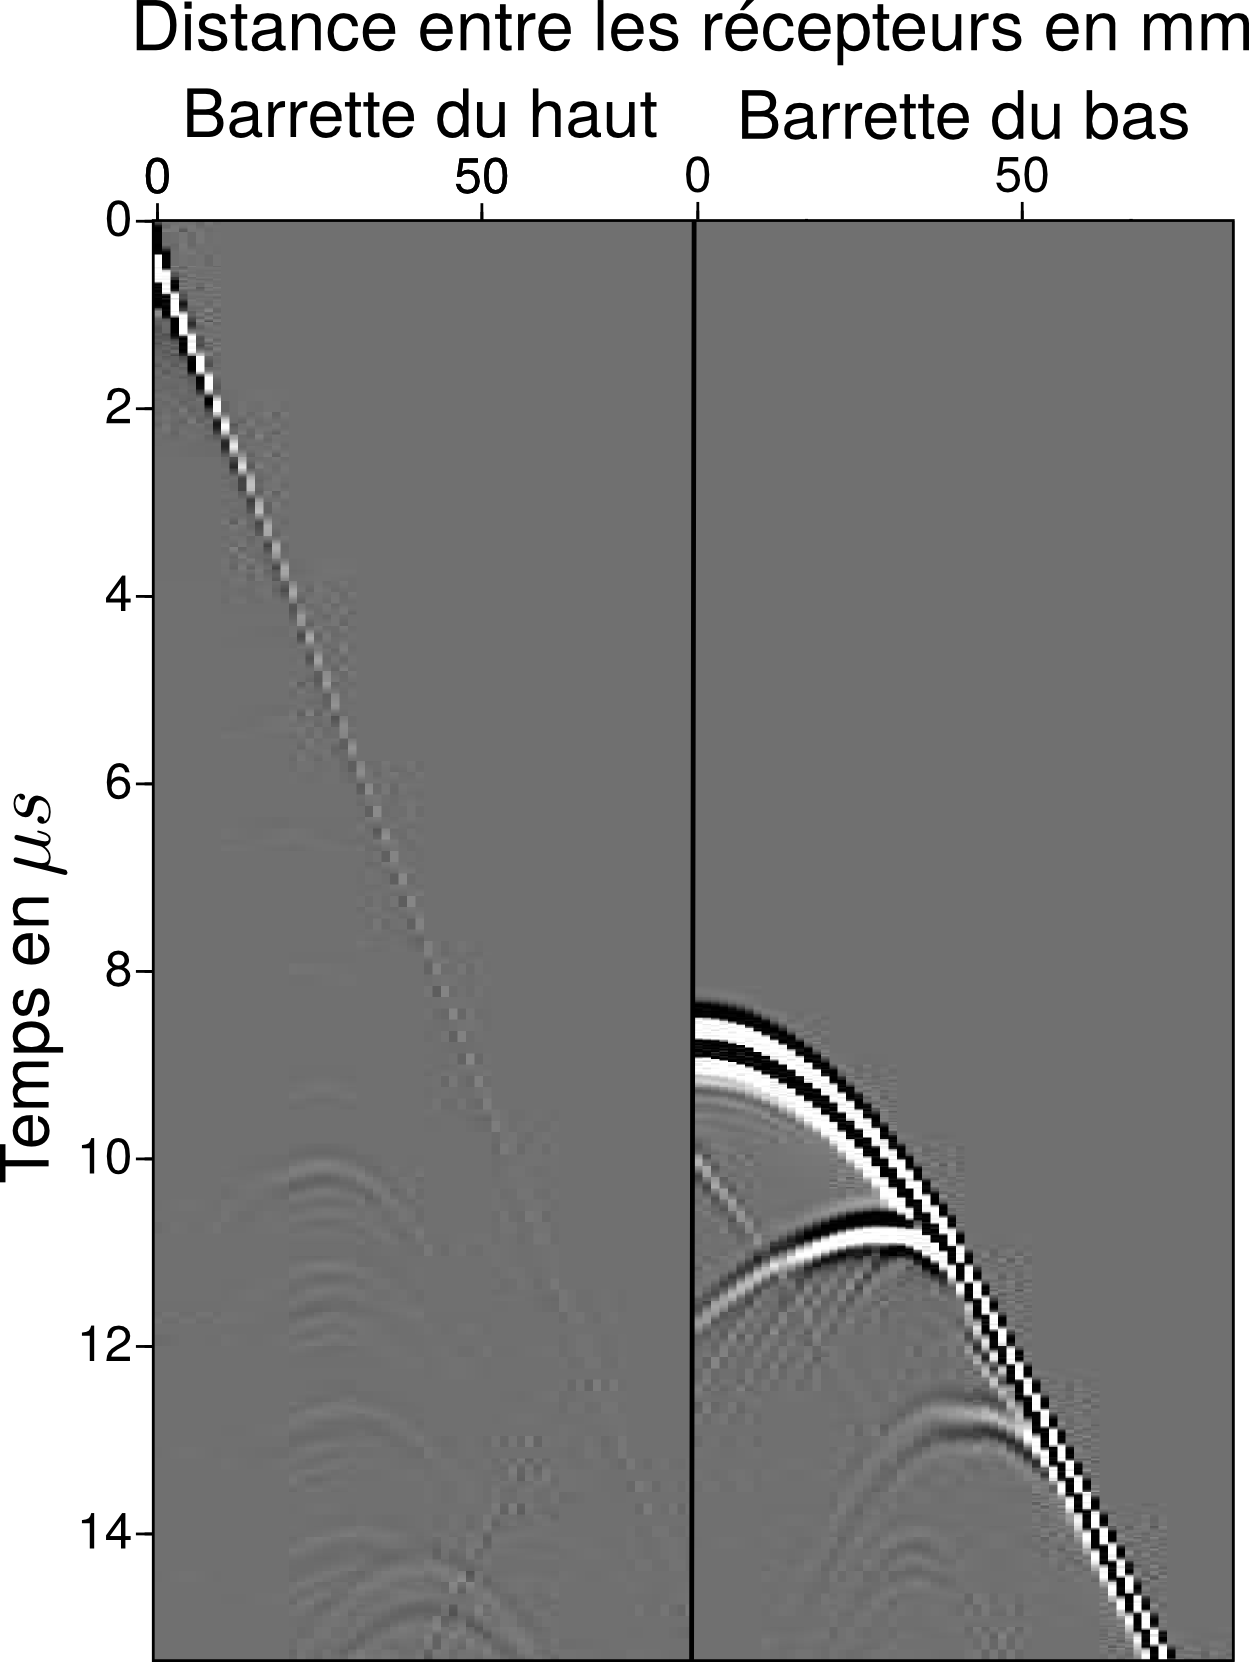
\includegraphics[height=4.3cm]{img/rho_mono/data_rho_uni.png}\\
		\scriptsize{Données issues d'une masse volumique homogène}
		\column{0.3\textwidth}
		\centering
		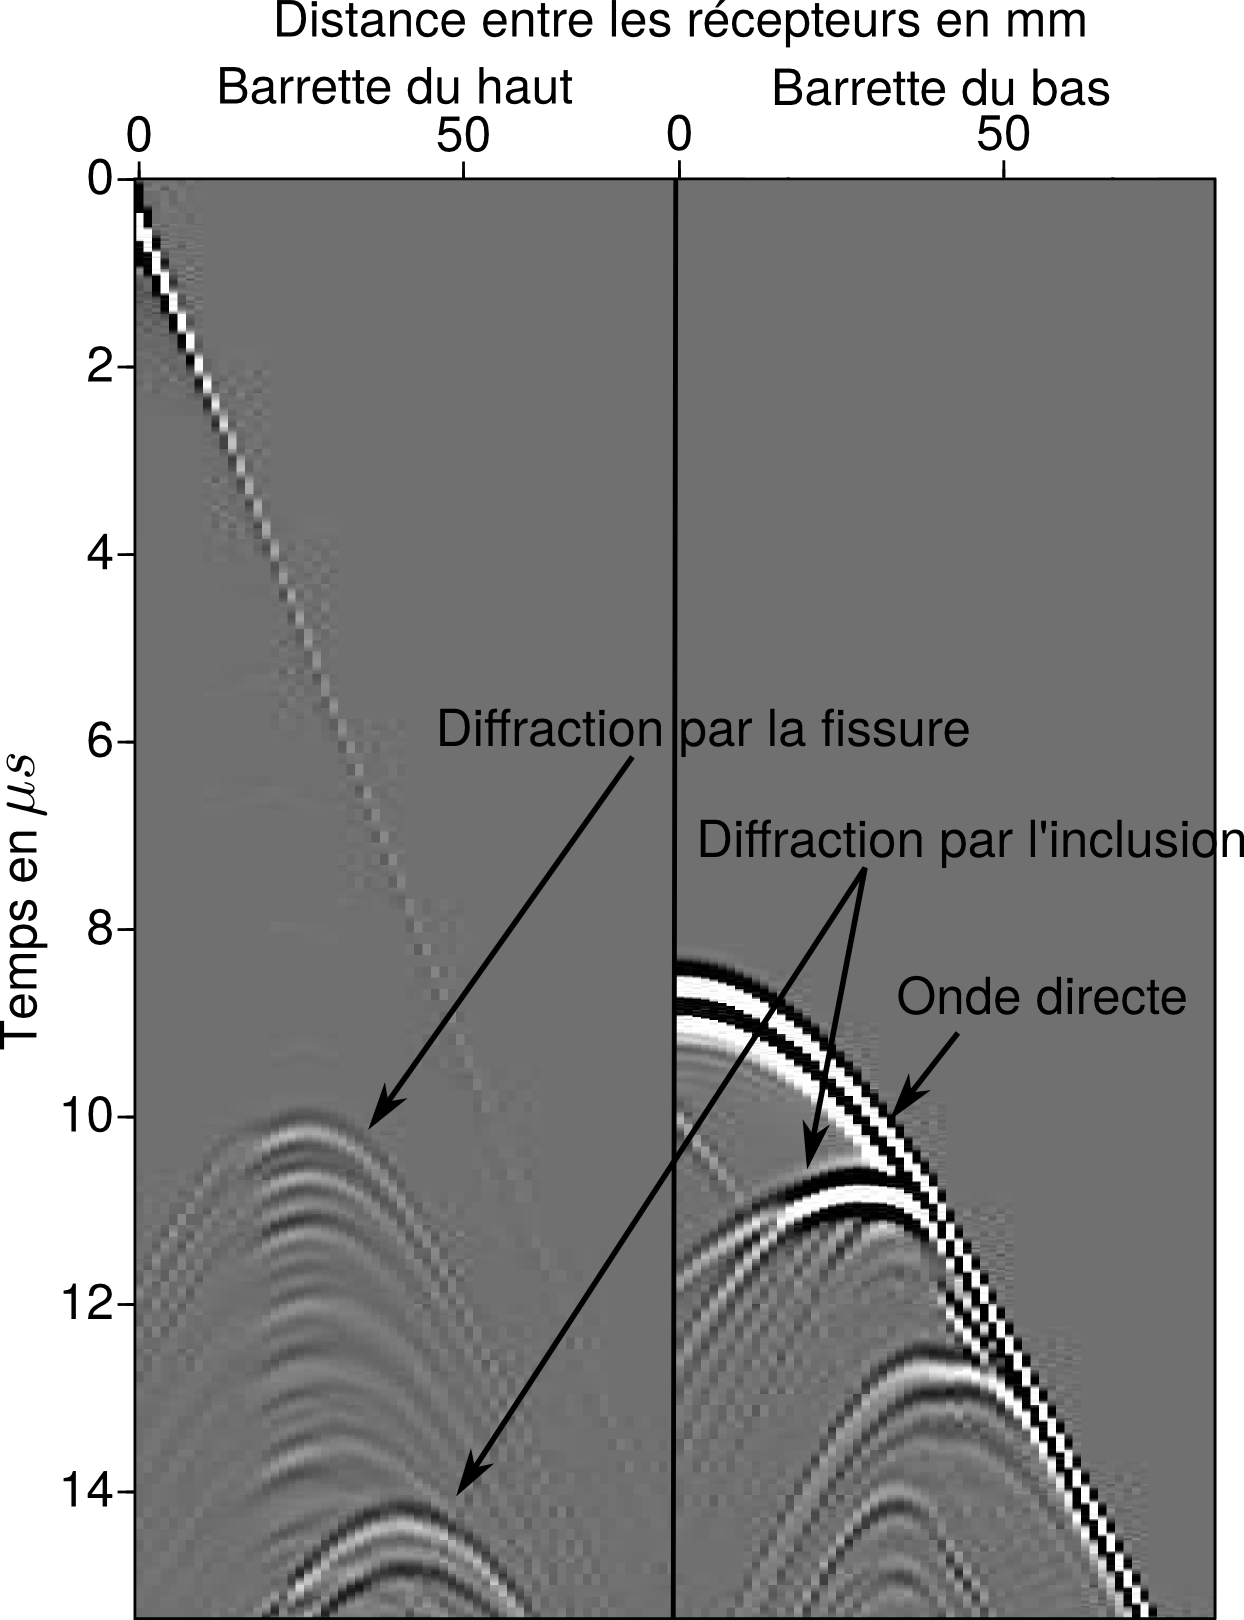
\includegraphics[height=4.3cm]{img/rho_mono/data_rho_vrai.png}\\
		\scriptsize{Données issues de la vraie masse volumique}
		}
	\end{columns}
	

\end{small}
\end{frame}

%\subsection{Inversion monoparamètre}
%\begin{frame}{\insertsectionhead~-- Vitesse}
%\begin{small}
%\centering
%	\begin{adjustwidth}{-2em}{-2.5em}
%	%\centering{Reconstruction de la vitesse}
%	\begin{columns}
%		\column{0.5\textwidth}
%		\centering
%		\vspace{0.1cm}\\	
%		Modèle initial de vitesse : \\[0.2cm]
%		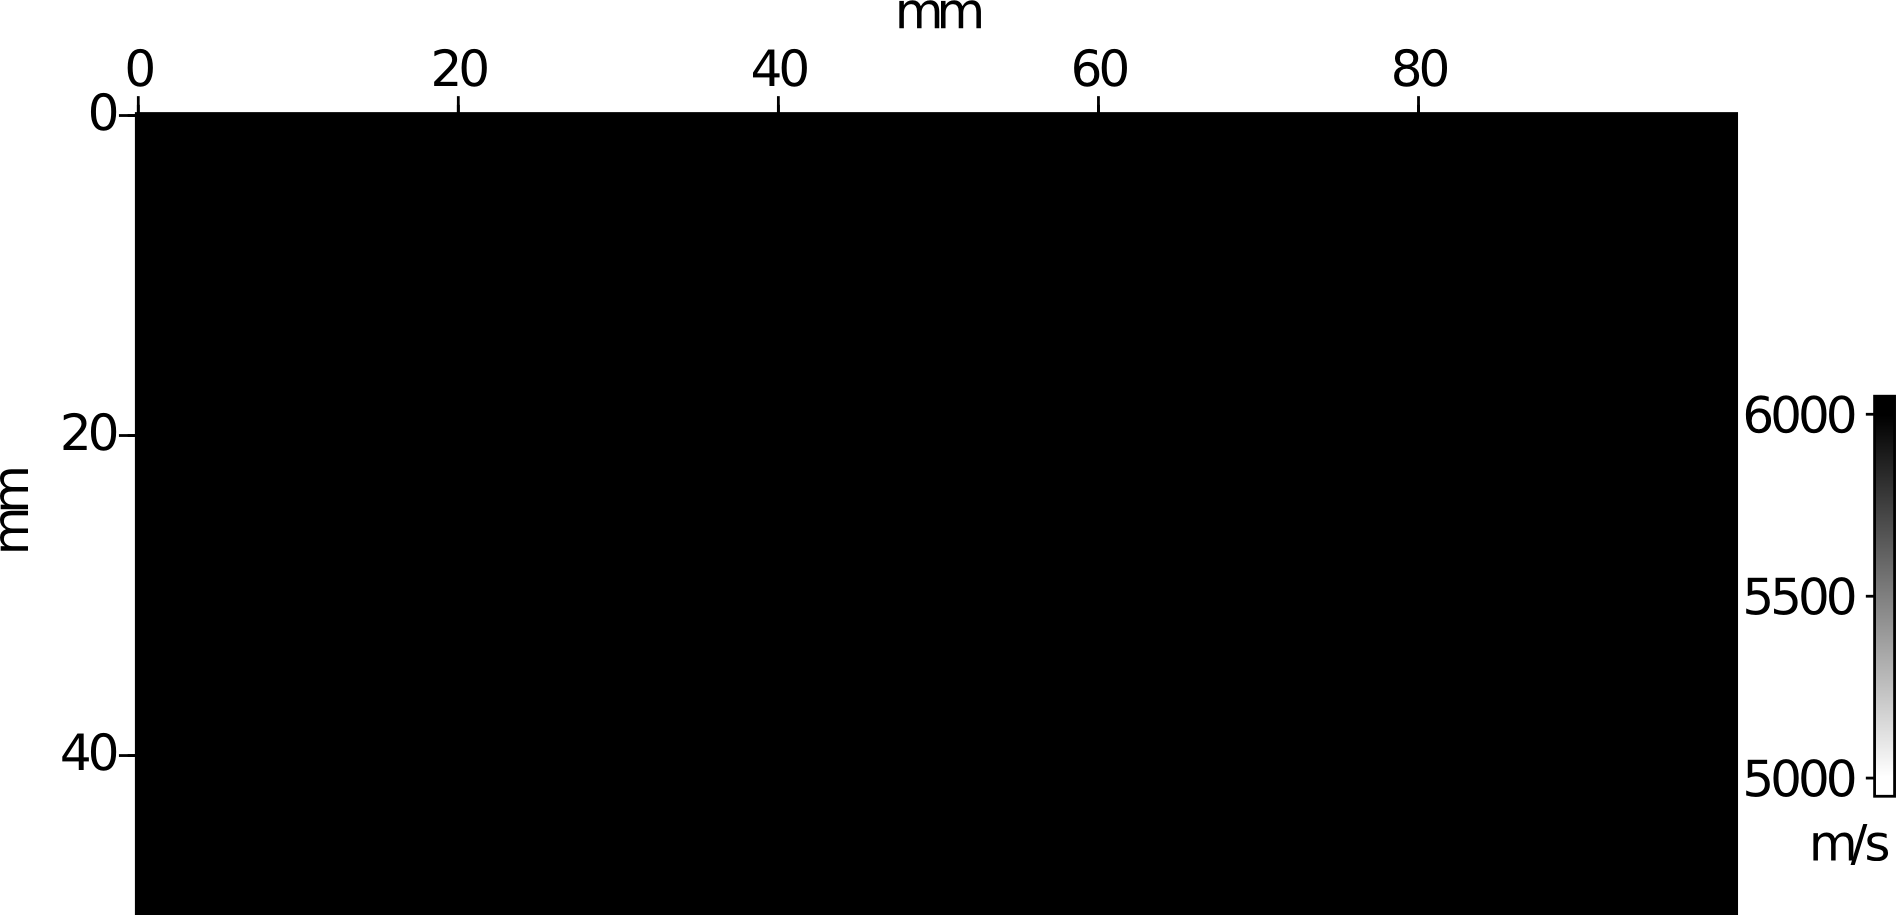
\includegraphics[width=0.7\textwidth]{img/vp_mono_uni/vp_uni.png}\\
%			\only<2->{\vspace{0.3cm}  Vitesse Reconstruite :\\[0.2cm]}
%			\only<1-1>{\vspace{2.7cm}}
%			\only<2-2>{
%				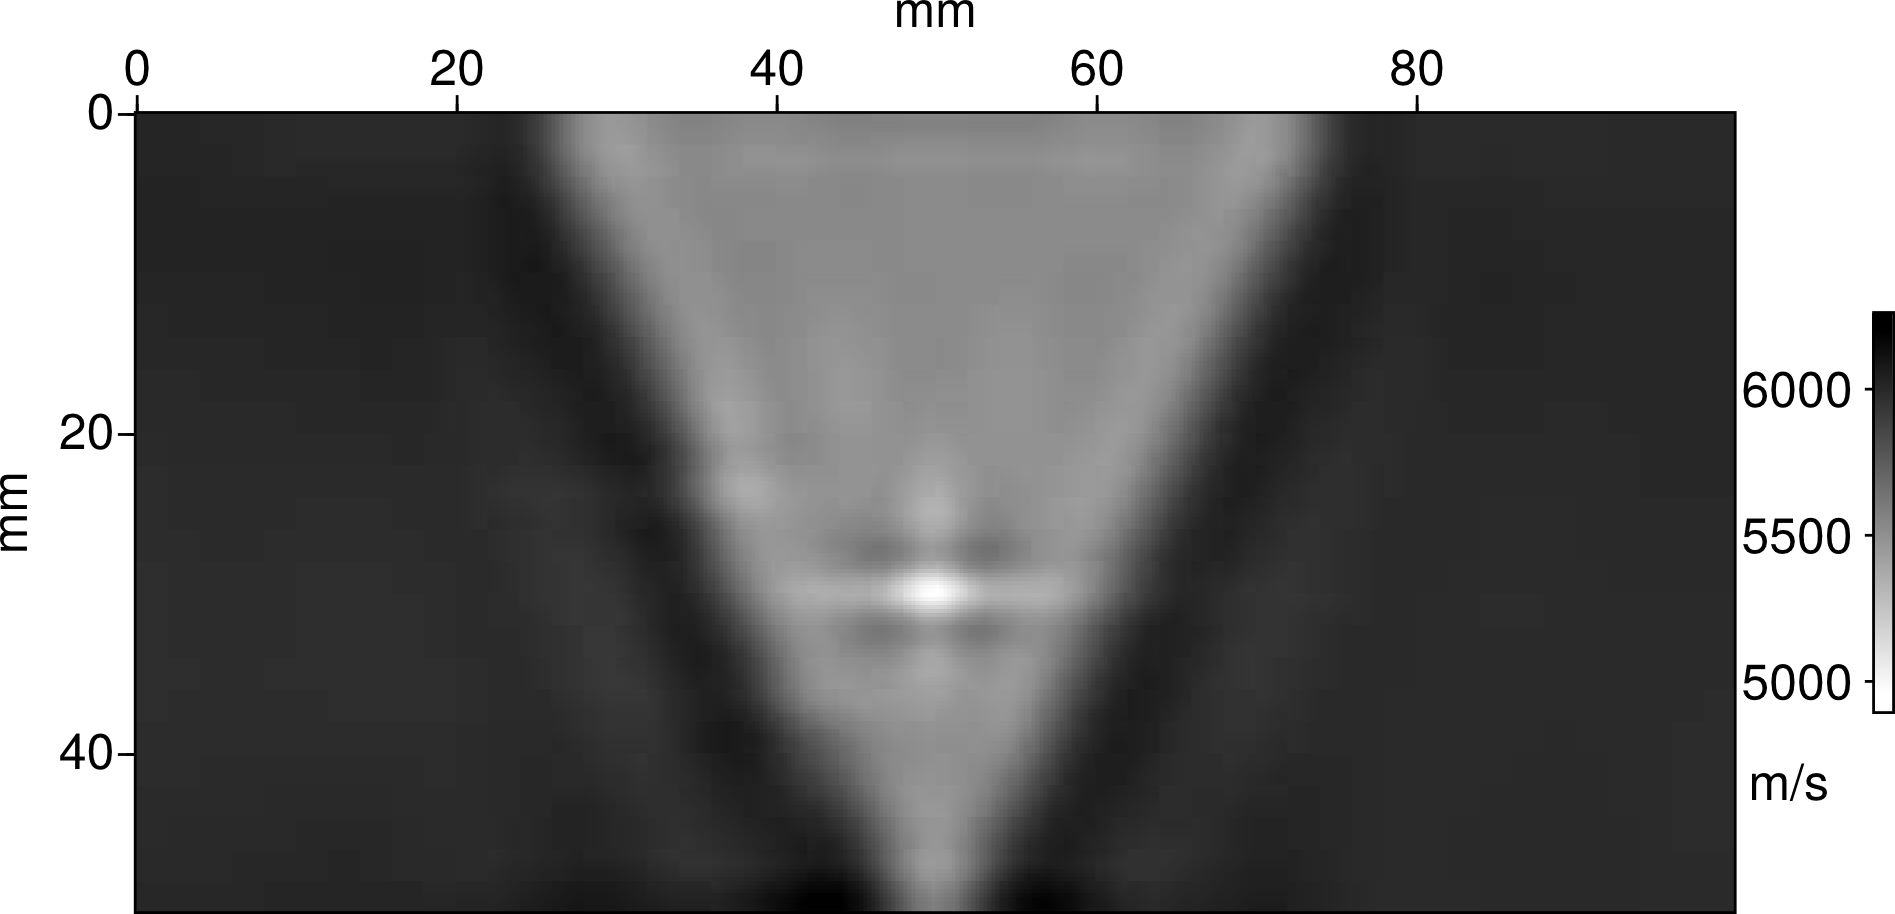
\includegraphics[width=0.7\textwidth]{img/vp_mono_uni/vp_450k.png}\\		
%			}
%		
%			\only<3-3>{
%				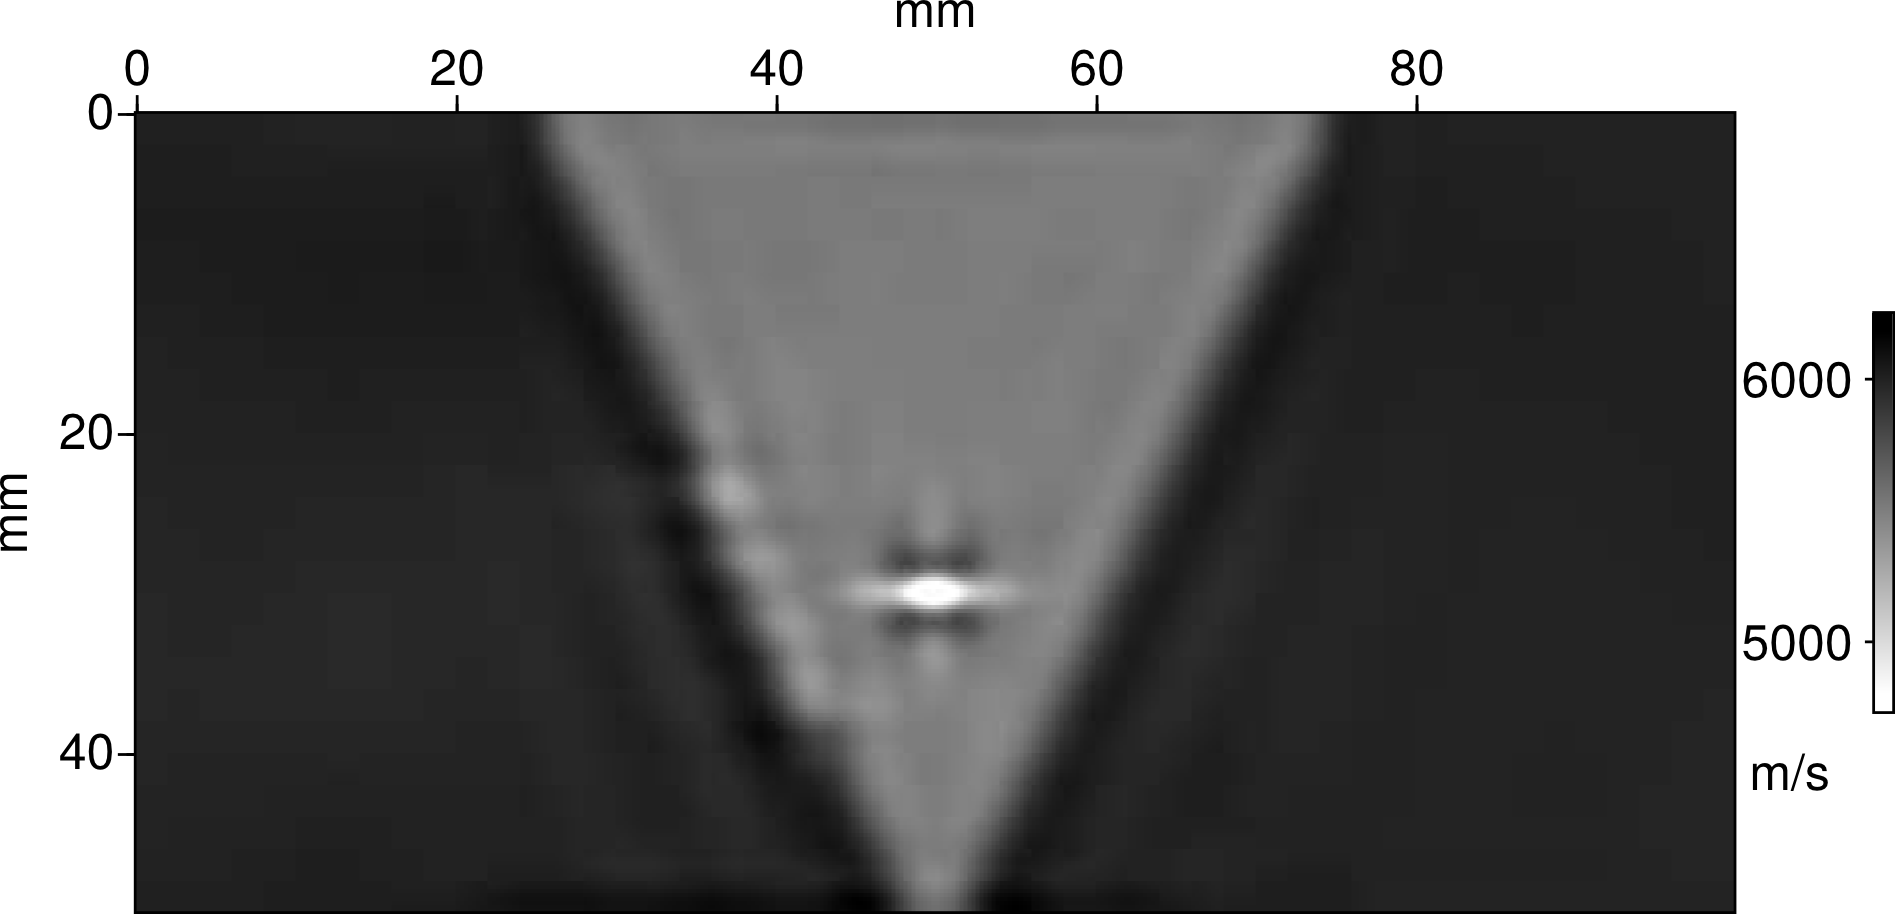
\includegraphics[width=0.7\textwidth]{img/vp_mono_uni/vp_1000k.png}\\		
%			}
%			\only<4-4>{
%				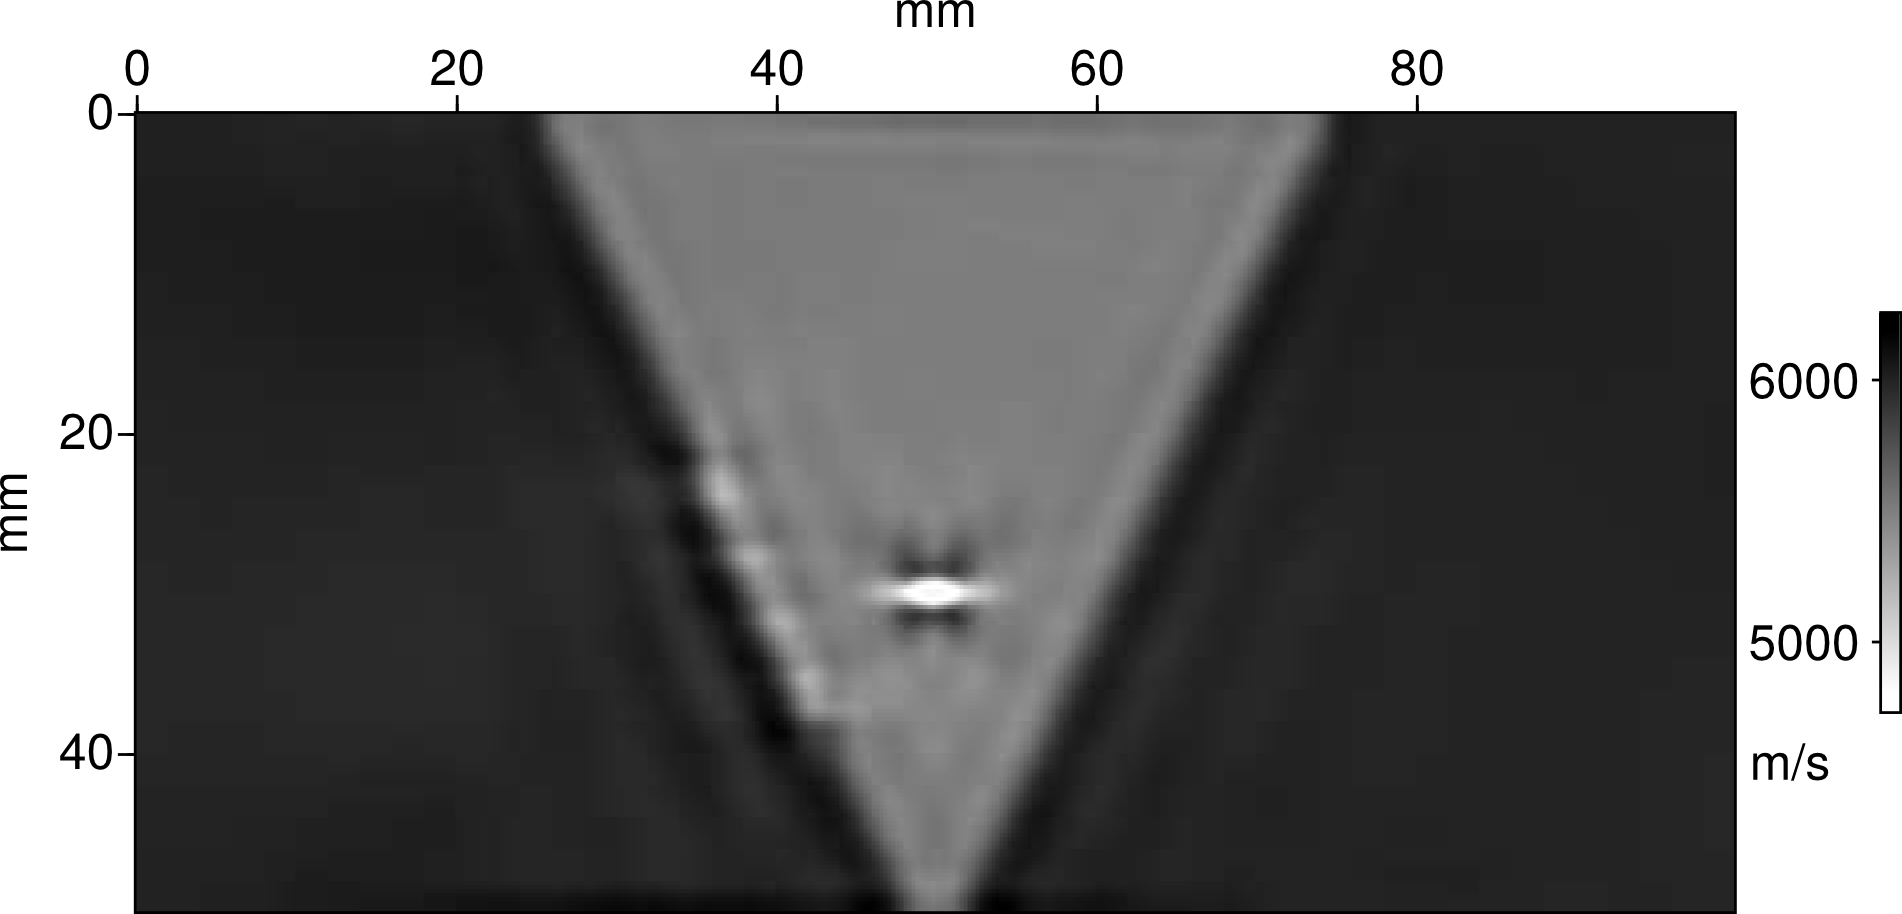
\includegraphics[width=0.7\textwidth]{img/vp_mono_uni/vp_1500k.png}\\		
%			}
%			\only<5-5>{
%				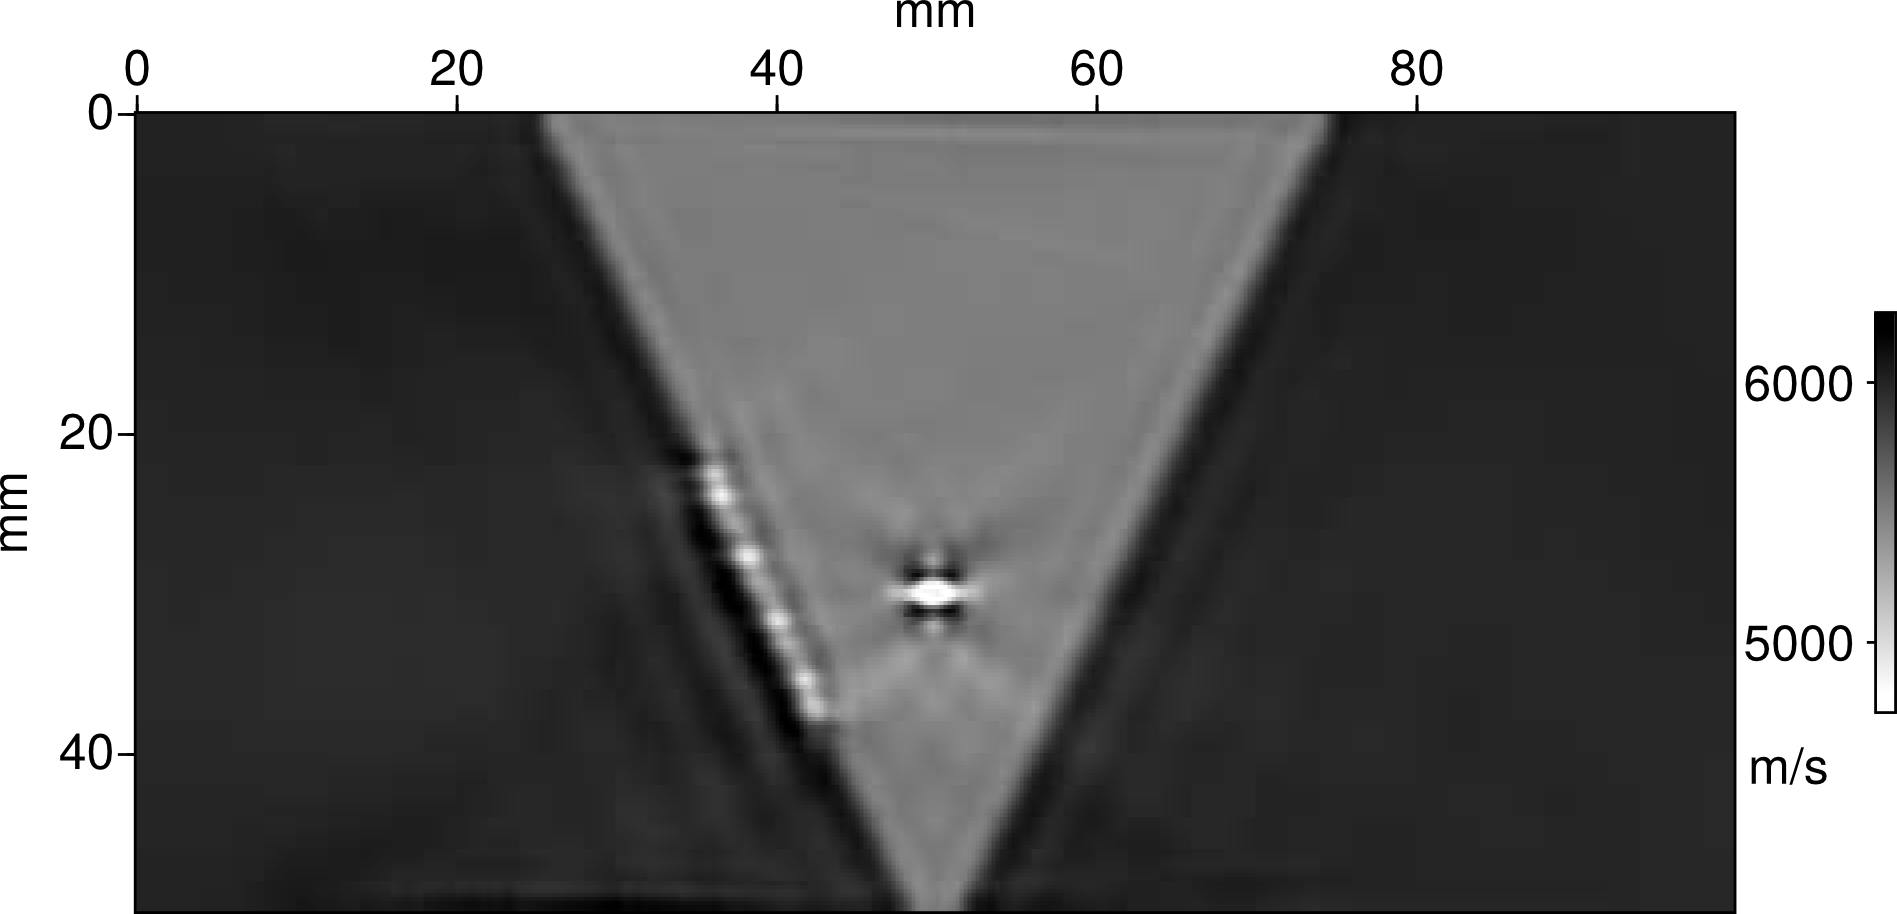
\includegraphics[width=0.7\textwidth]{img/vp_mono_uni/vp_2250k.png}\\		
%			}
%			\only<6->{
%				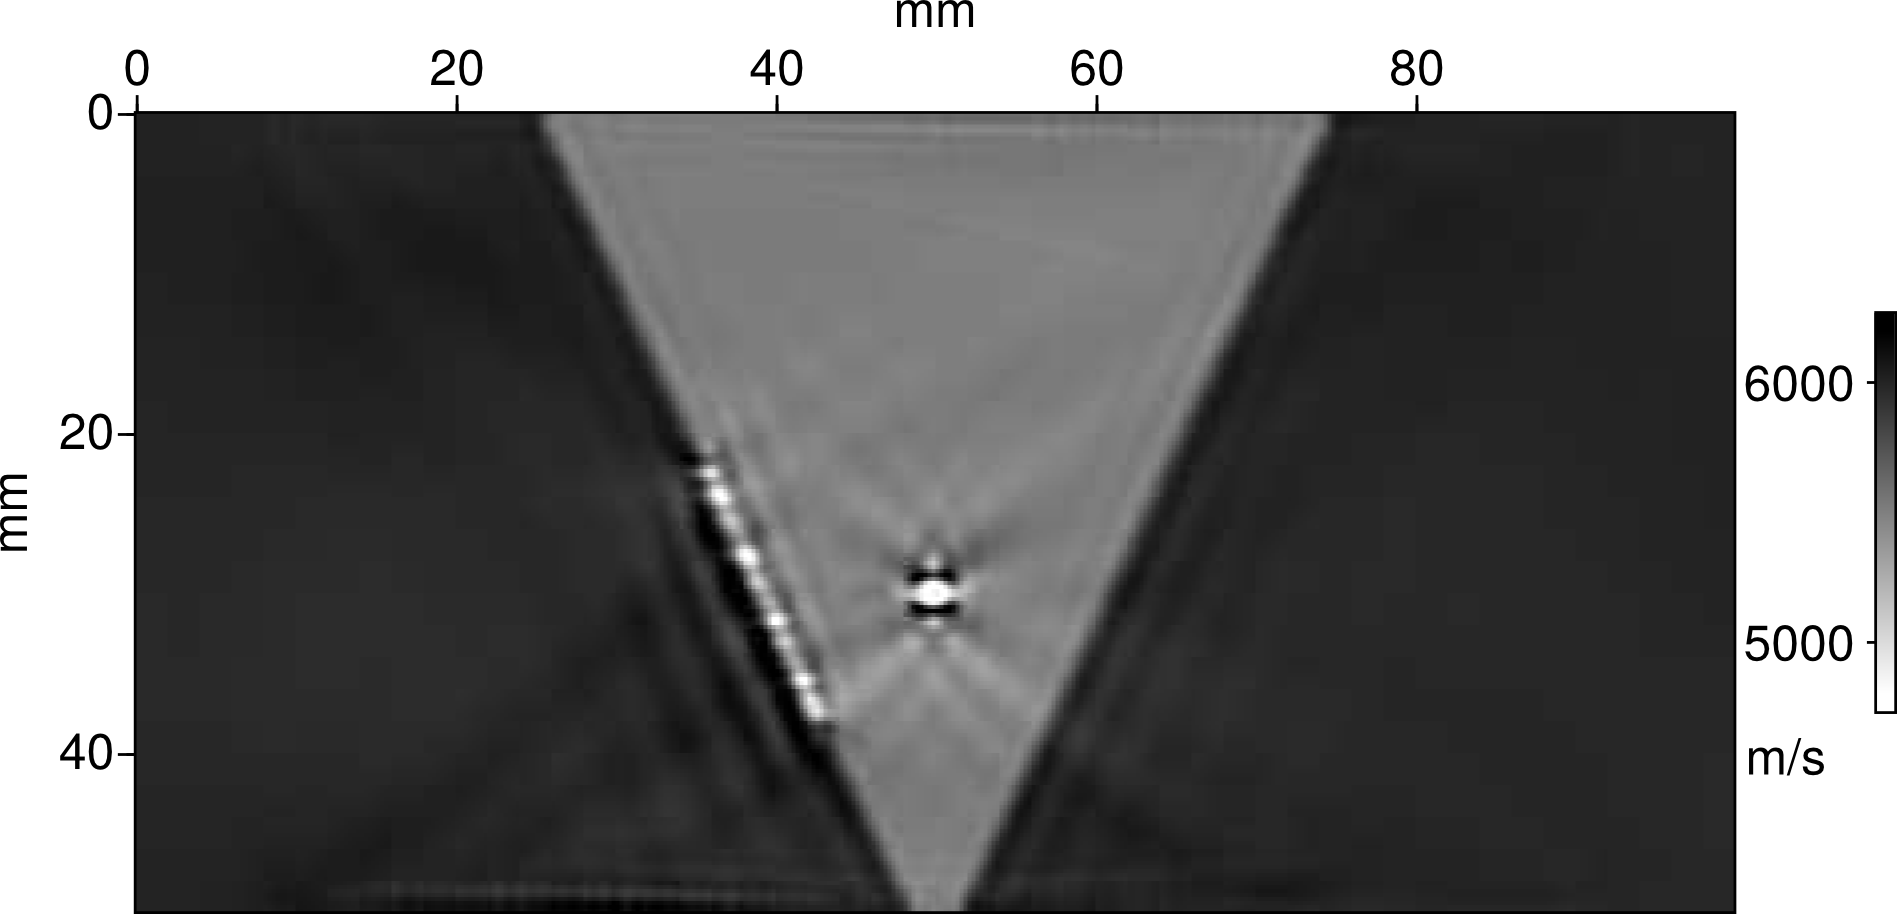
\includegraphics[width=0.7\textwidth]{img/vp_mono_uni/vp_3300k.png}\\		
%			}
%		
%
%		\column{0.5\textwidth}
%		\centering
%		\vspace{0.1cm}\\
%		Modèle initial de vitesse :\\[0.2cm]
%		\includegraphics[width=0.7\textwidth]{img/vp_mono_smooth/vp_smooth.png}\\
%		\only<2->{\vspace{0.3cm} Vitesse Reconstruite :\\[0.2cm]}
%		\only<1-1>{\vspace{2.7cm}}
%		\only<2-2>{
%			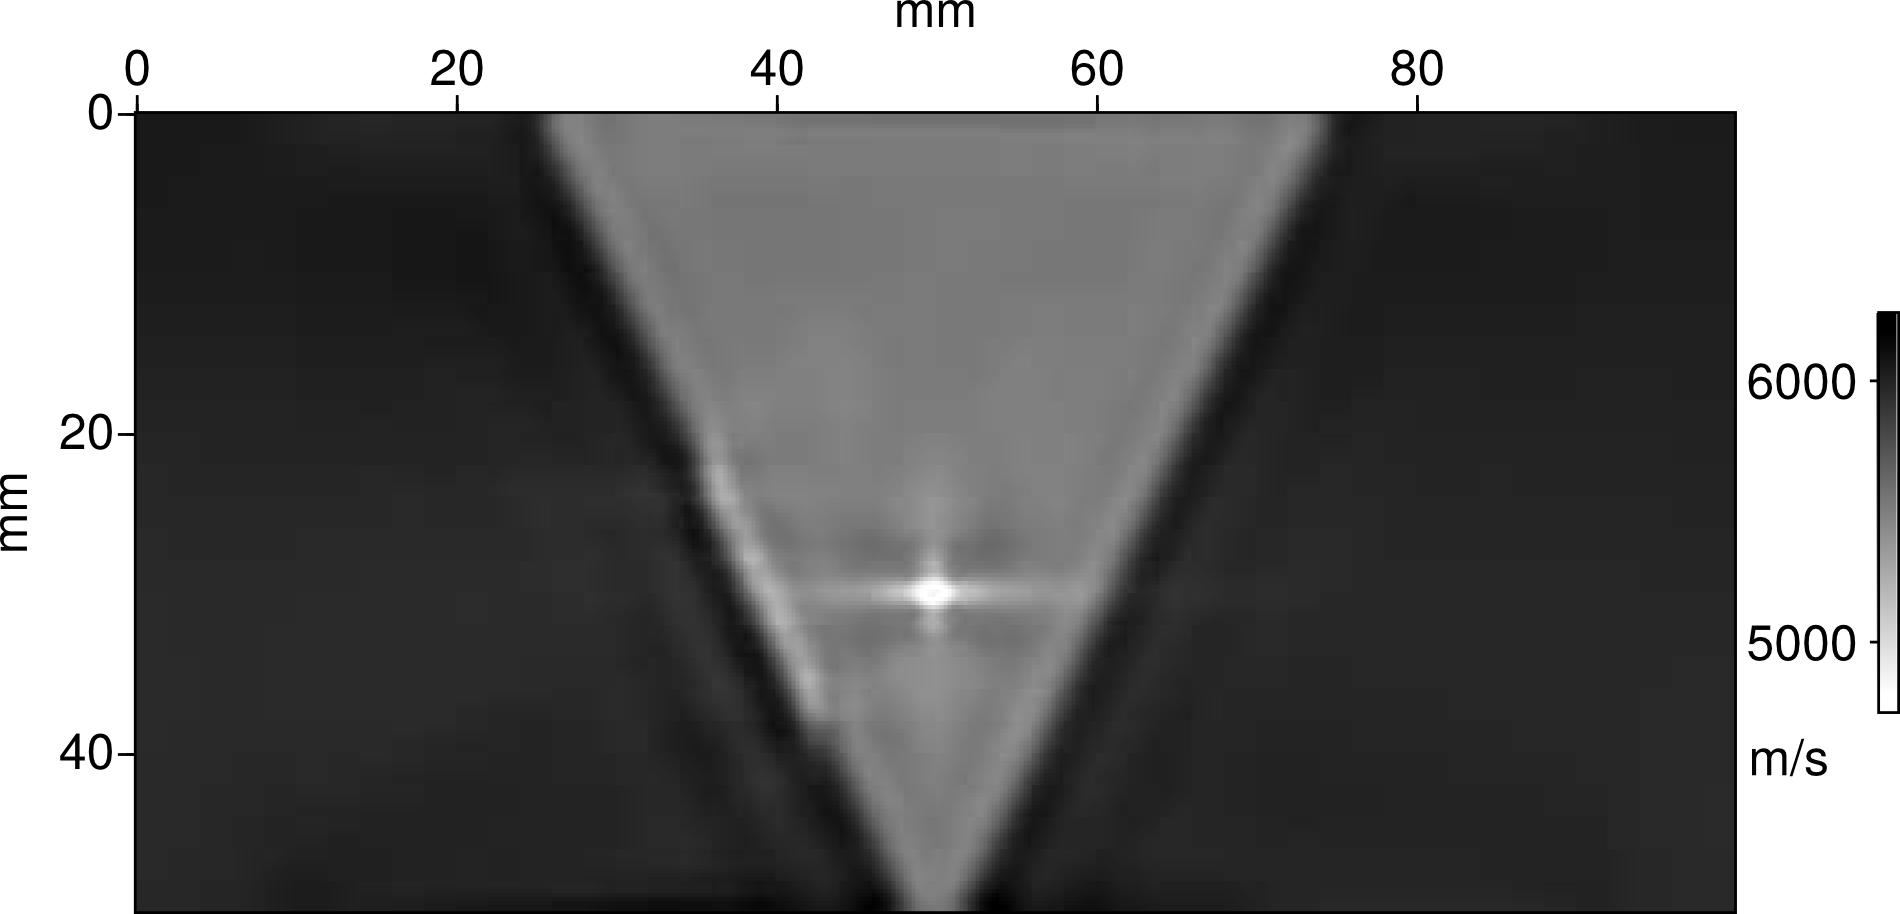
\includegraphics[width=0.7\textwidth]{img/vp_mono_smooth/vp_400k.png}\\		
%		}
%		\only<3-3>{
%			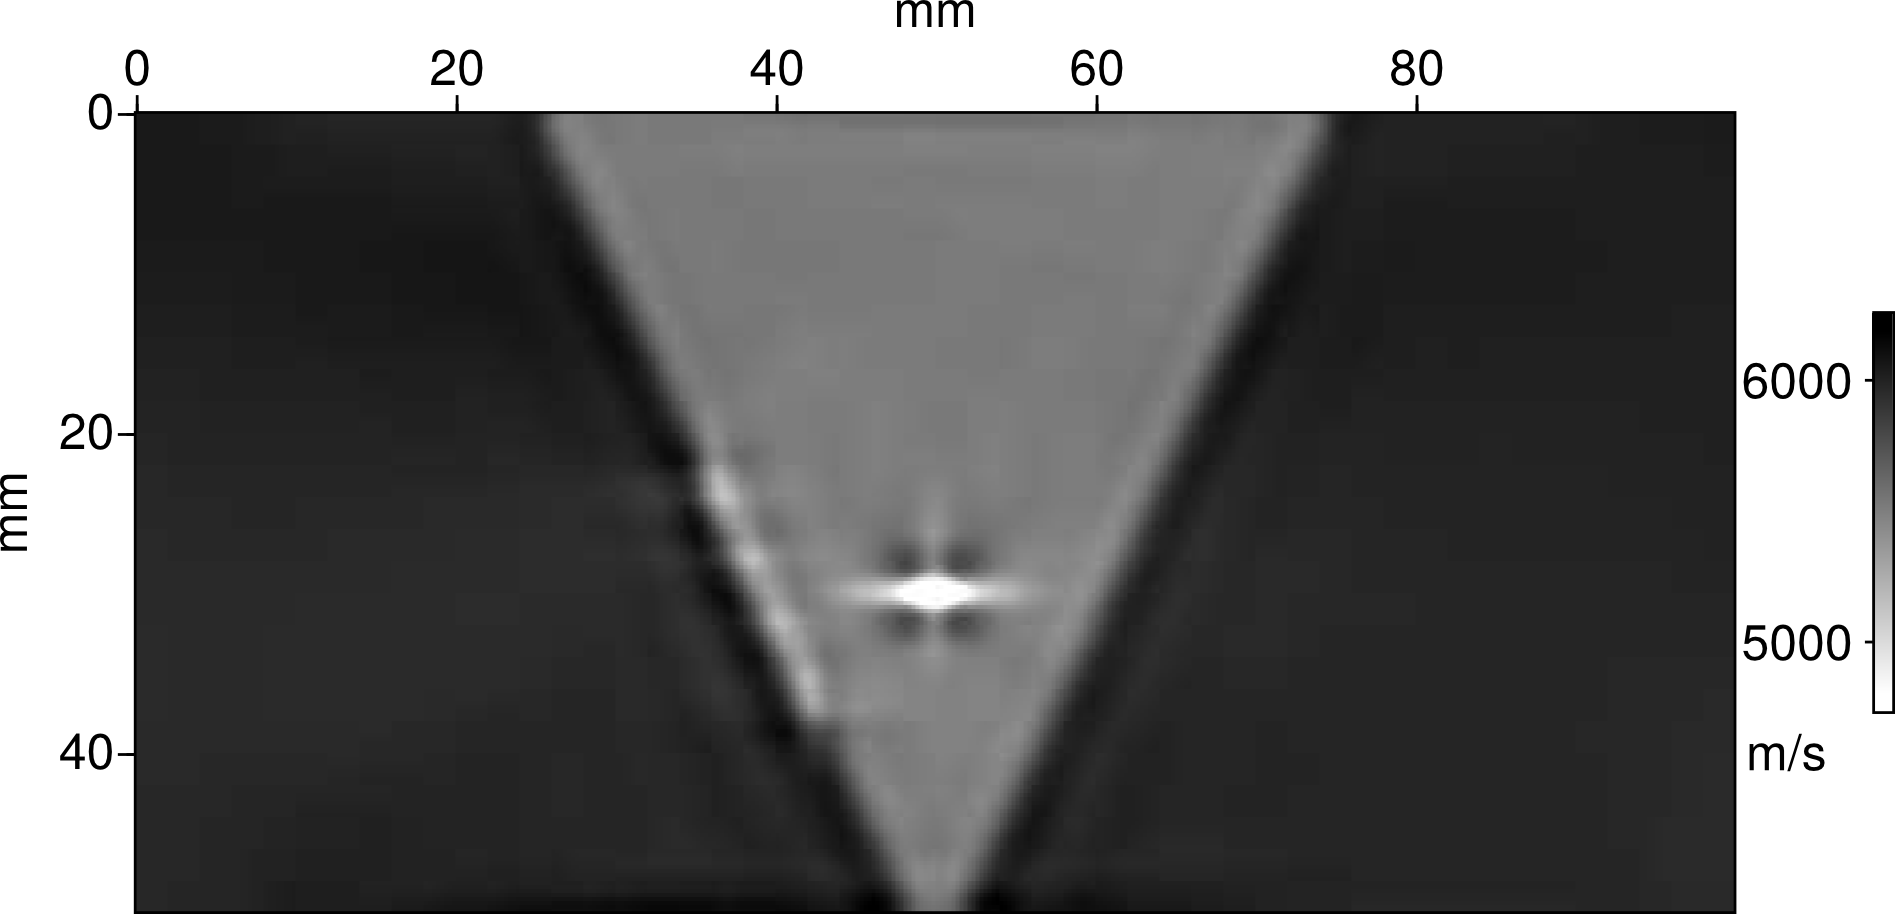
\includegraphics[width=0.7\textwidth]{img/vp_mono_smooth/vp_900k.png}\\		
%		}
%		\only<4-4>{
%			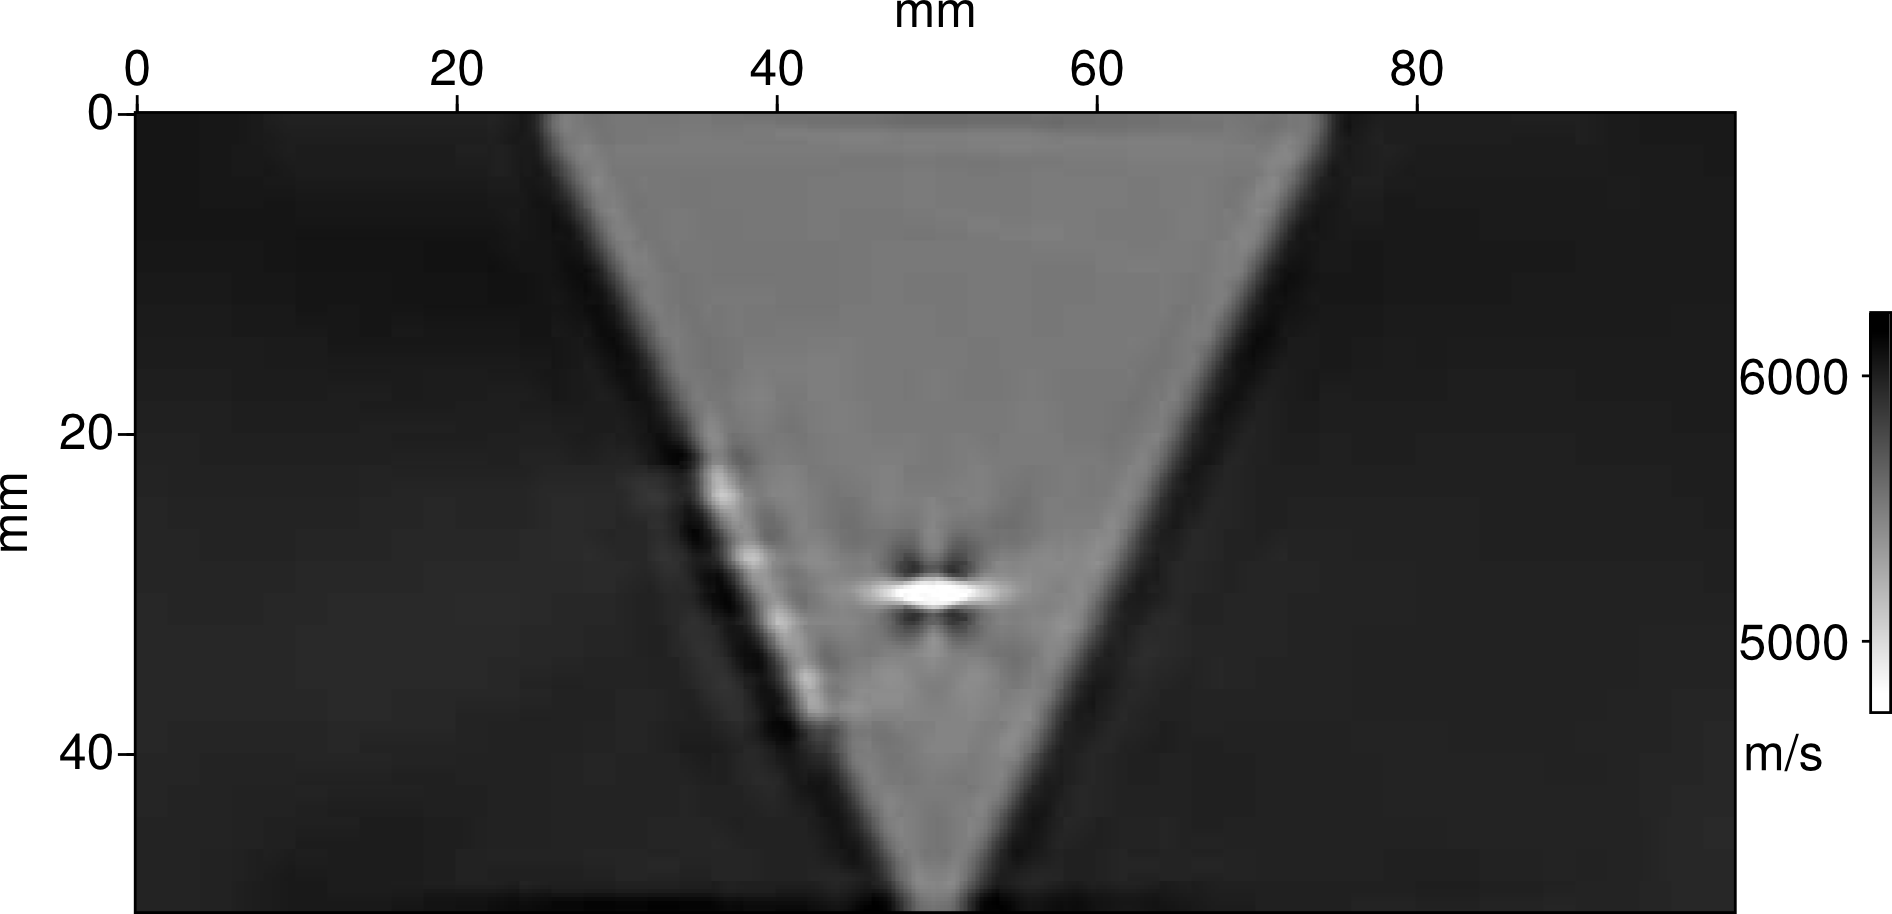
\includegraphics[width=0.7\textwidth]{img/vp_mono_smooth/vp_1300k.png}\\		
%		}
%		\only<5-5>{
%			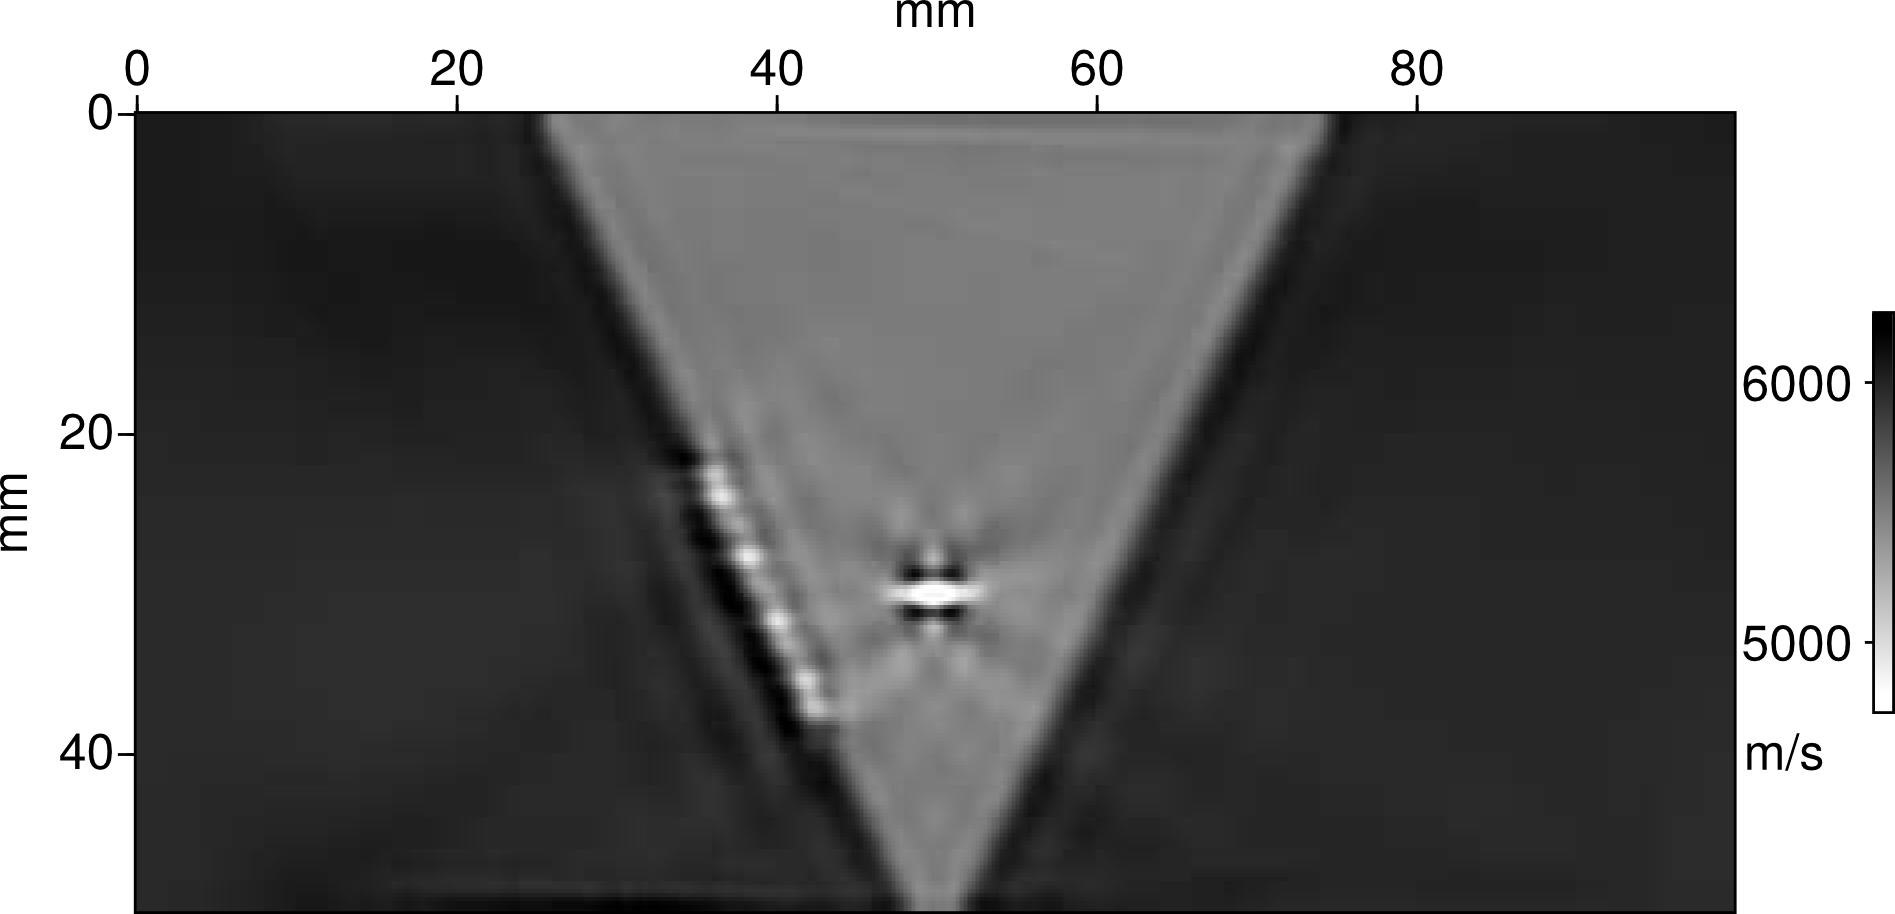
\includegraphics[width=0.7\textwidth]{img/vp_mono_smooth/vp_1950k.png}\\		
%		}
%		\only<6->{
%			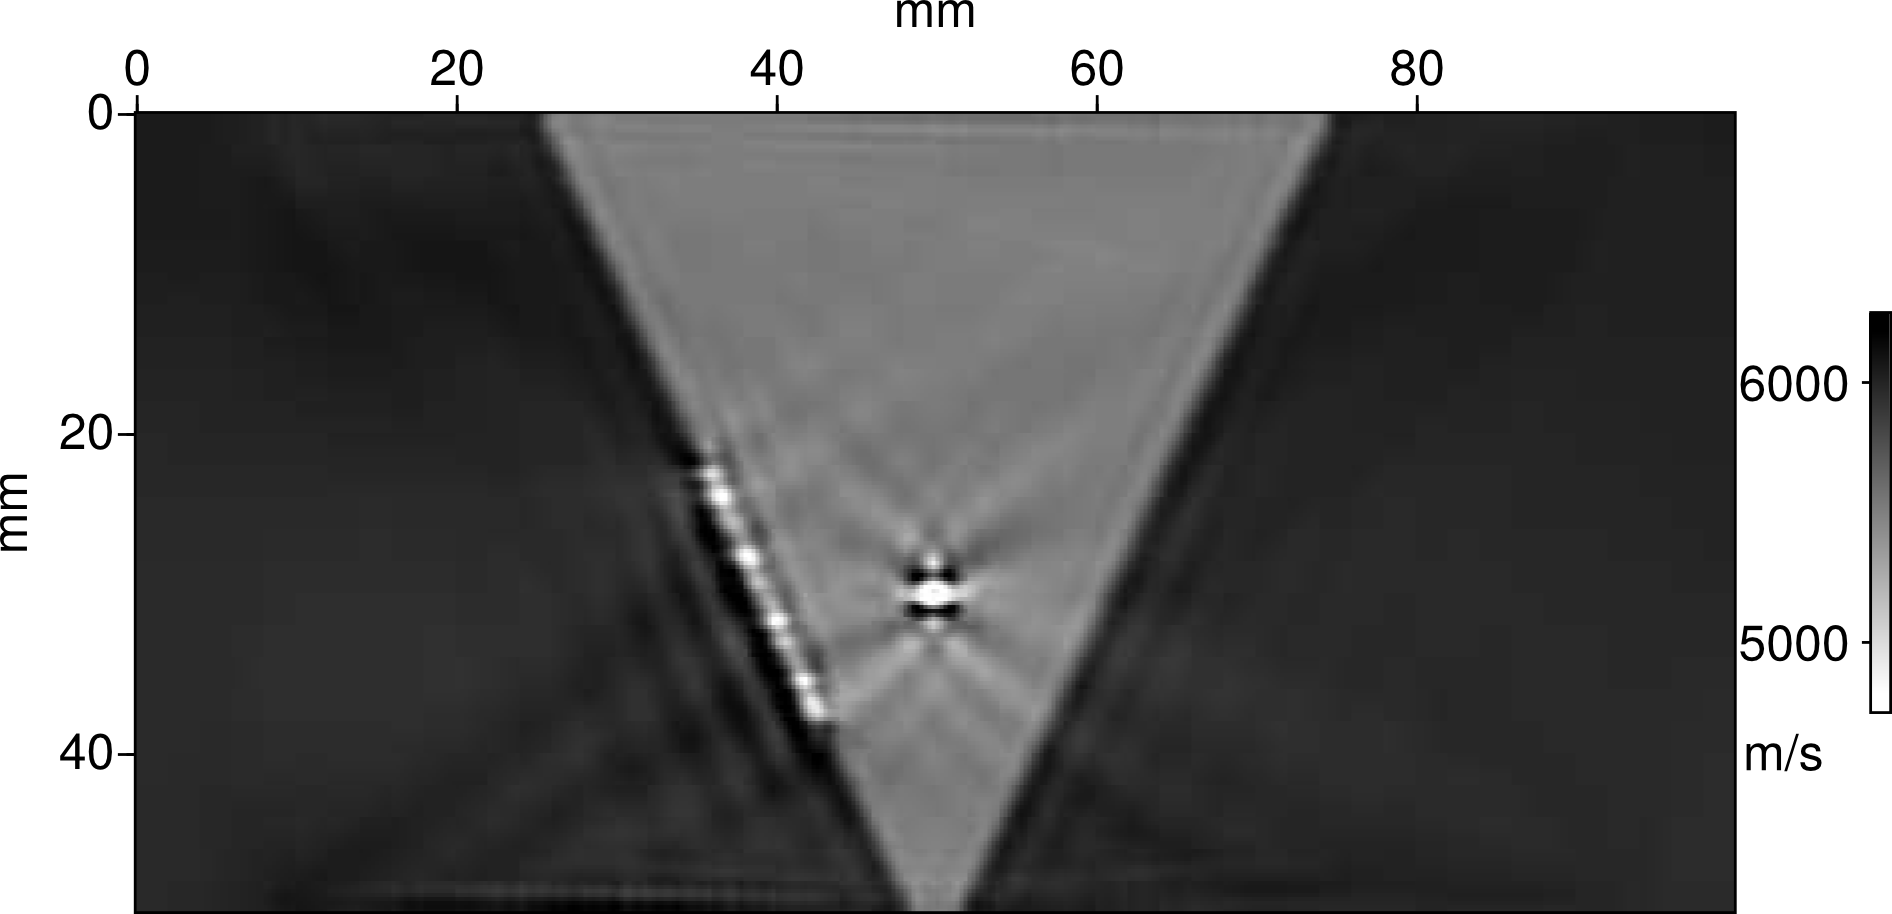
\includegraphics[width=0.7\textwidth]{img/vp_mono_smooth/vp_2900k.png}\\		
%		}
%		
%		
%	\end{columns}
%	\end{adjustwidth}
%	%\vspace{0.3cm} 
%	Vitesse vraie :
%	\begin{figure}
%		\centering
%		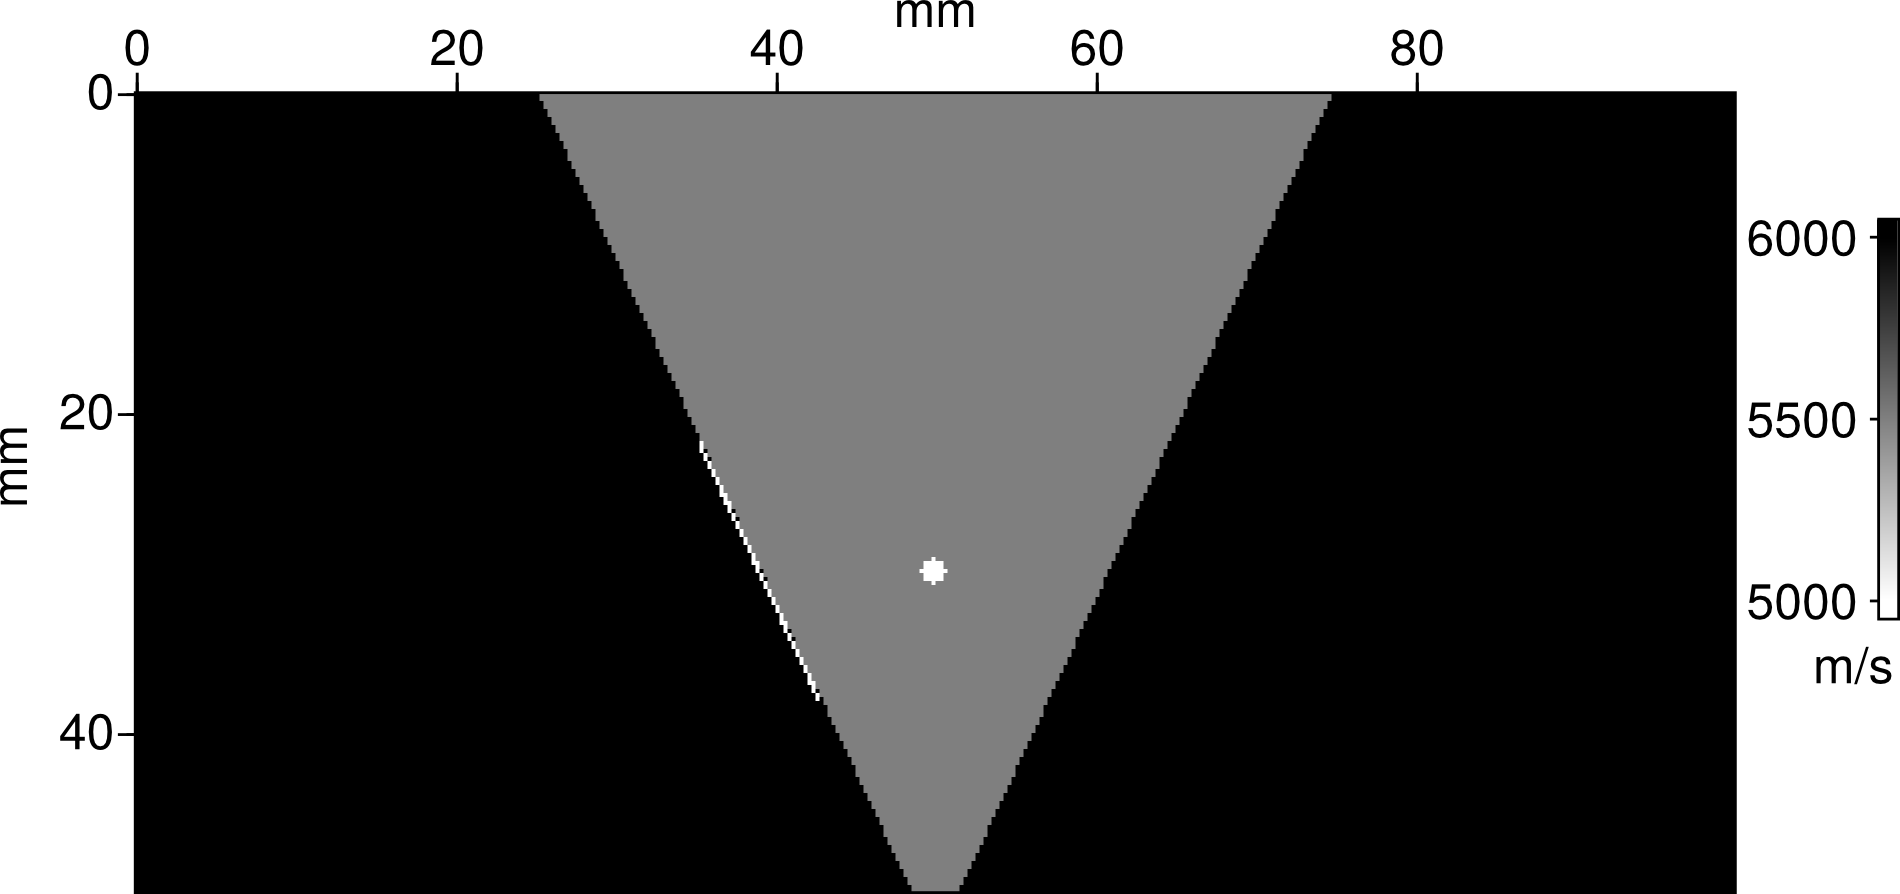
\includegraphics[width=0.35\textwidth]{img/vp_true_sans_acqui.png}\\
%	\end{figure}
%	
%	\begin{picture}(0,0)(0,0)\put(127,120){
%		\only<2-2>{f$\approx$ 400 kHz}
%		\only<3-3>{f$\approx$ 1 MHz~}
%		\only<4-4>{\hspace{-0.1cm}f$\approx$ 1,4 MHz~~}
%		\only<5-5>{\hspace{-0.2cm}f$\approx$ 2 MHz~~~}
%		\only<6-6>{\hspace{-0.2cm}f$\approx$ 3 MHz}
%	}\end{picture}
%\end{small}
%\end{frame}

%\subsection*{}
%\begin{frame}{\insertsectionhead~-- Densité}
%\begin{footnotesize}
%
%		\centering
%		\begin{columns}
%			\column{0.5\textwidth}
%			\raggedleft
%			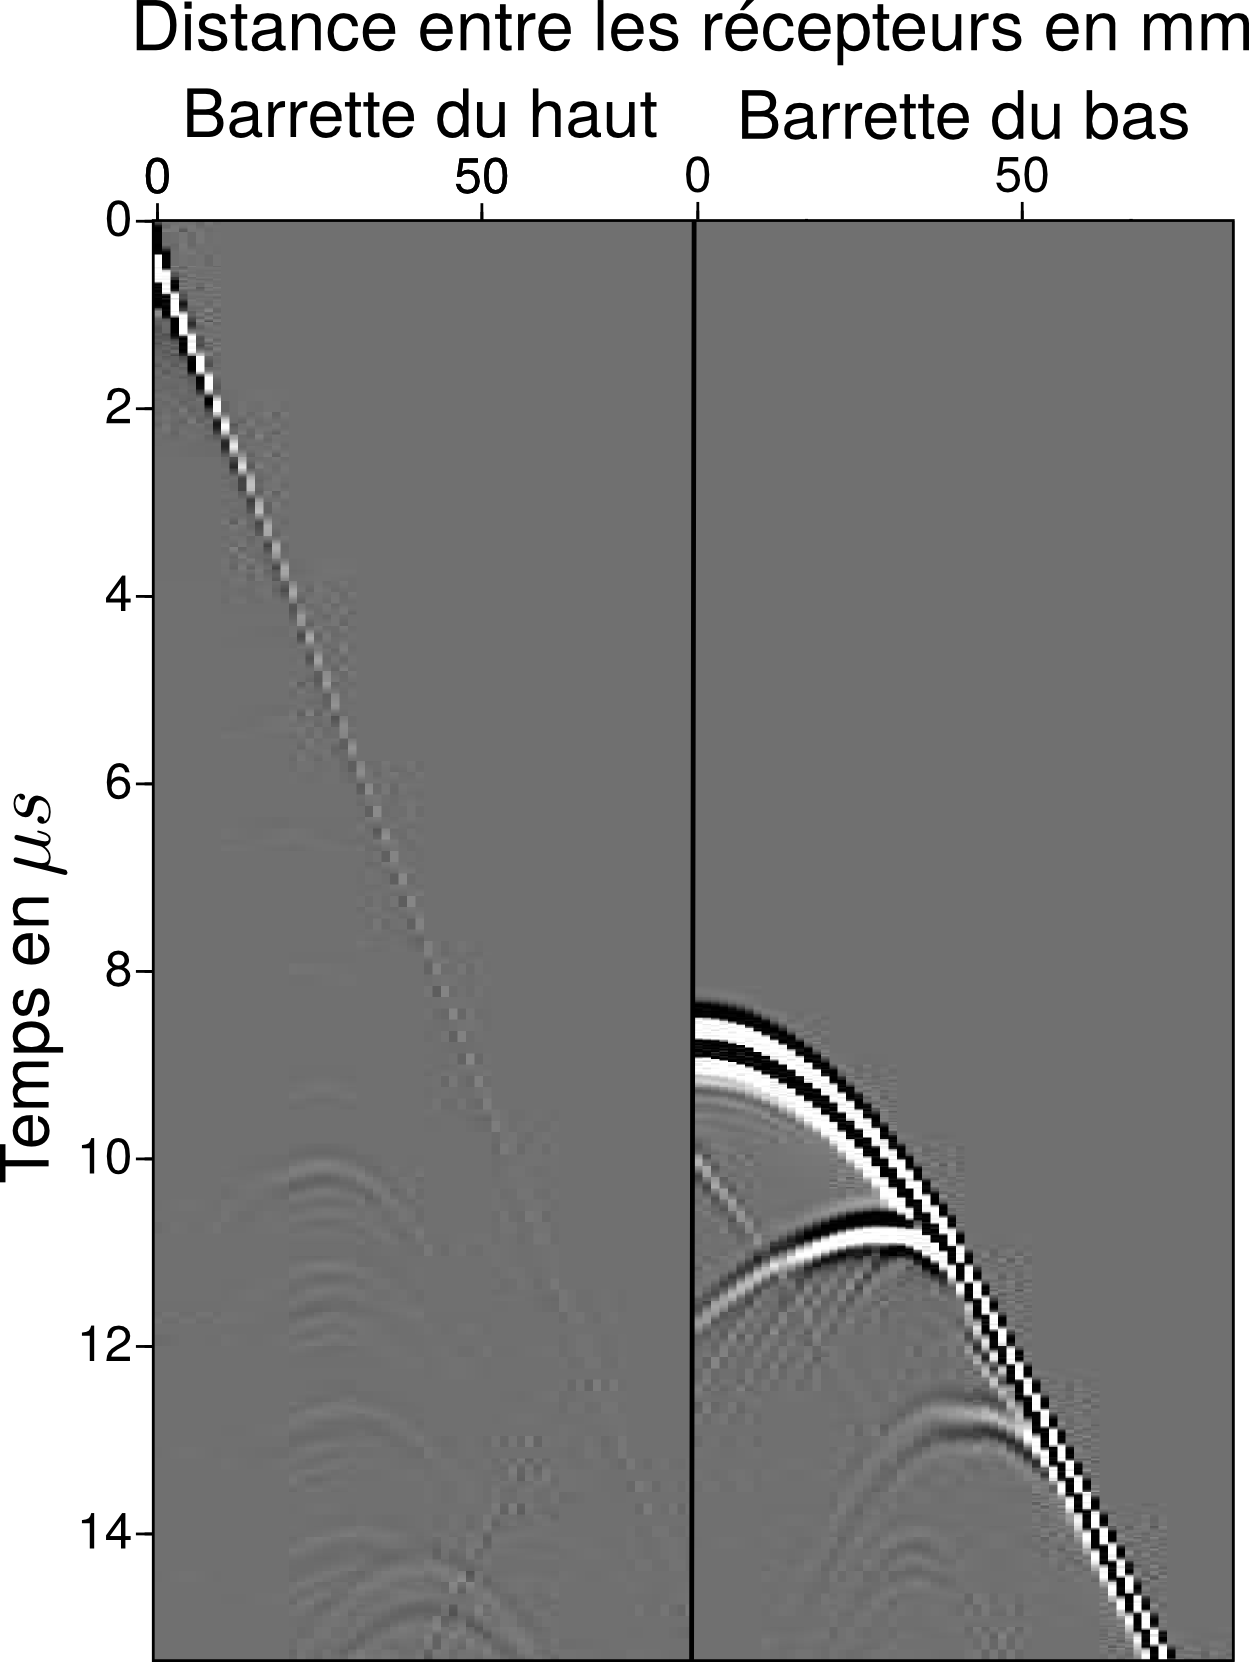
\includegraphics[width=3cm]{img/rho_mono/data_rho_uni.png}\\
%			Signaux issus de $\rho$ homogène\hspace{-0.5cm}
%			\column{0.5\textwidth}
%			\raggedright
%			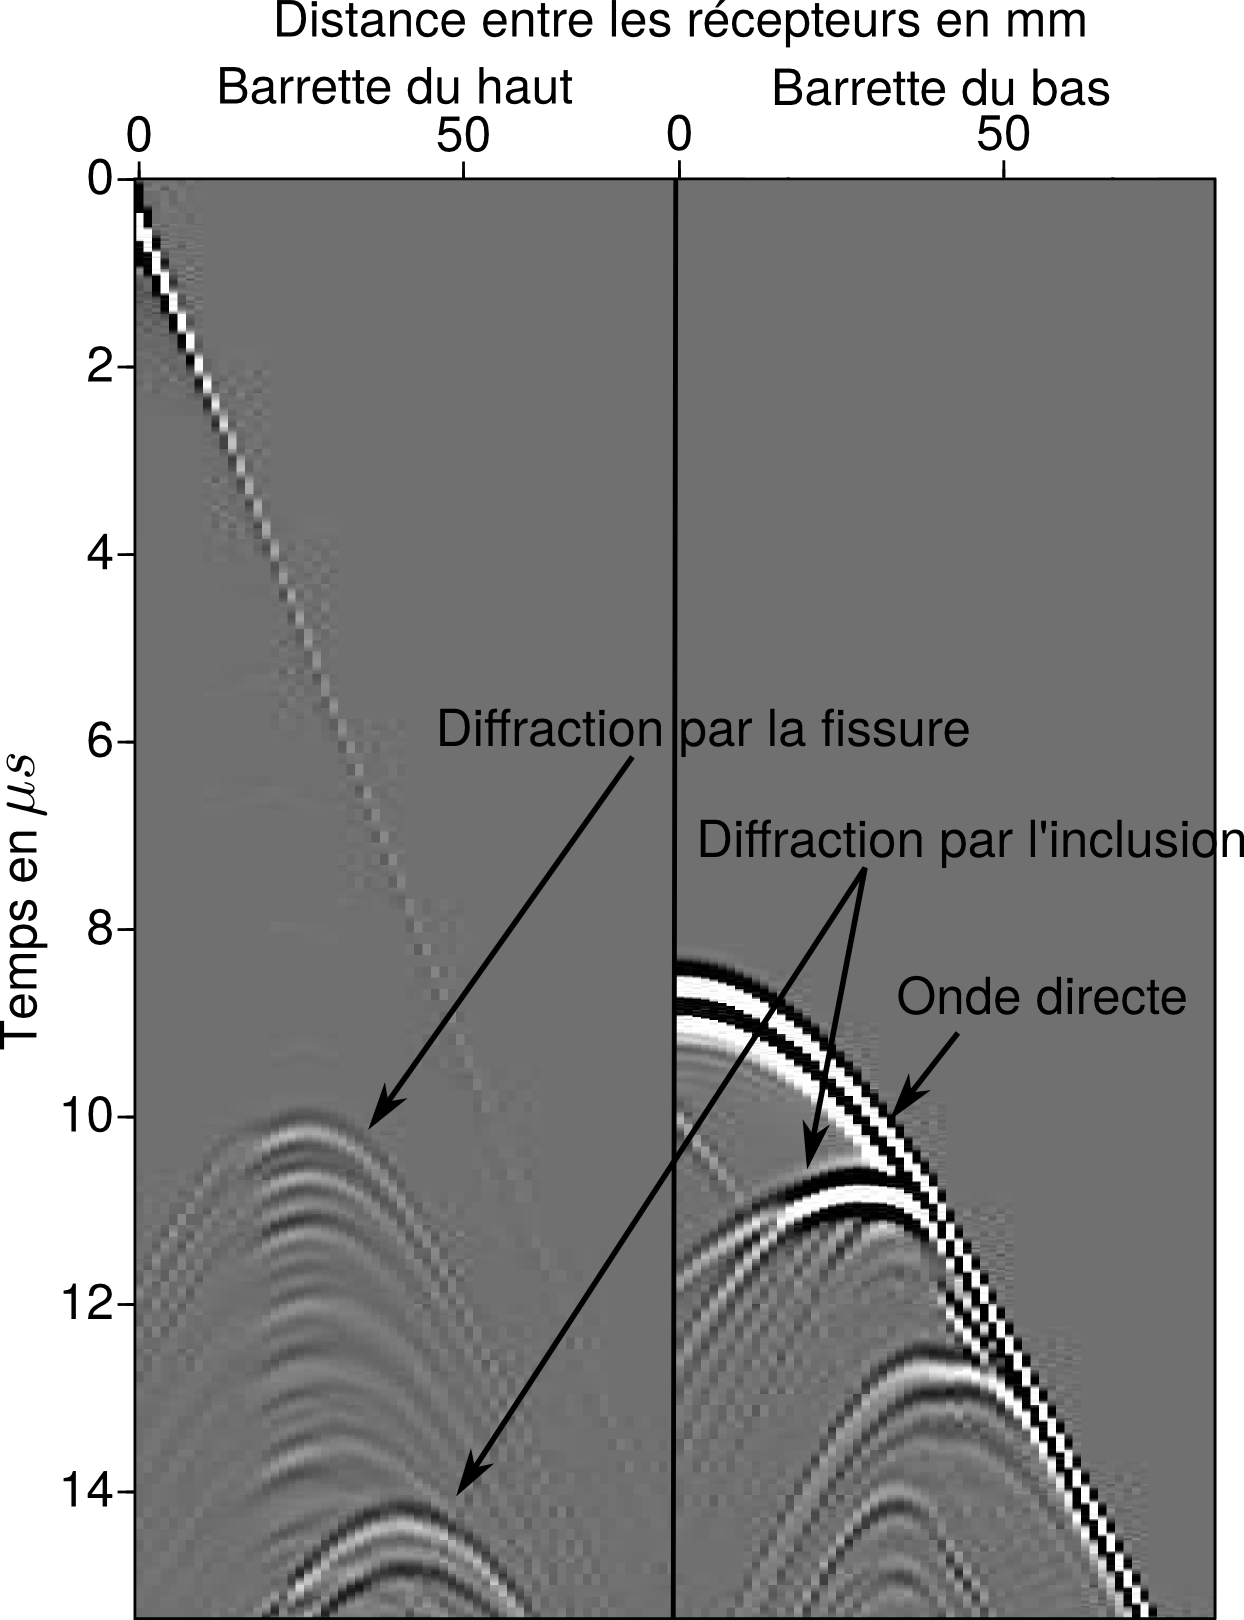
\includegraphics[width=3cm]{img/rho_mono/data_rho_vrai.png}\\
%			~~~Signaux issus de $\rho$ vraie
%		\end{columns}		
%		\vfill
%		
%		\begin{columns}
%			\column{0.35\textwidth}	
%			\centering
%			Modèle initial de vitesse : \\[0.2cm]
%			\includegraphics[width=\textwidth]{img/vp_mono_smooth/vp_smooth.png}\\
%			
%			\column{0.35\textwidth}
%			\centering
%			Masse volumique reconstruite :  \\[0.2cm]
%			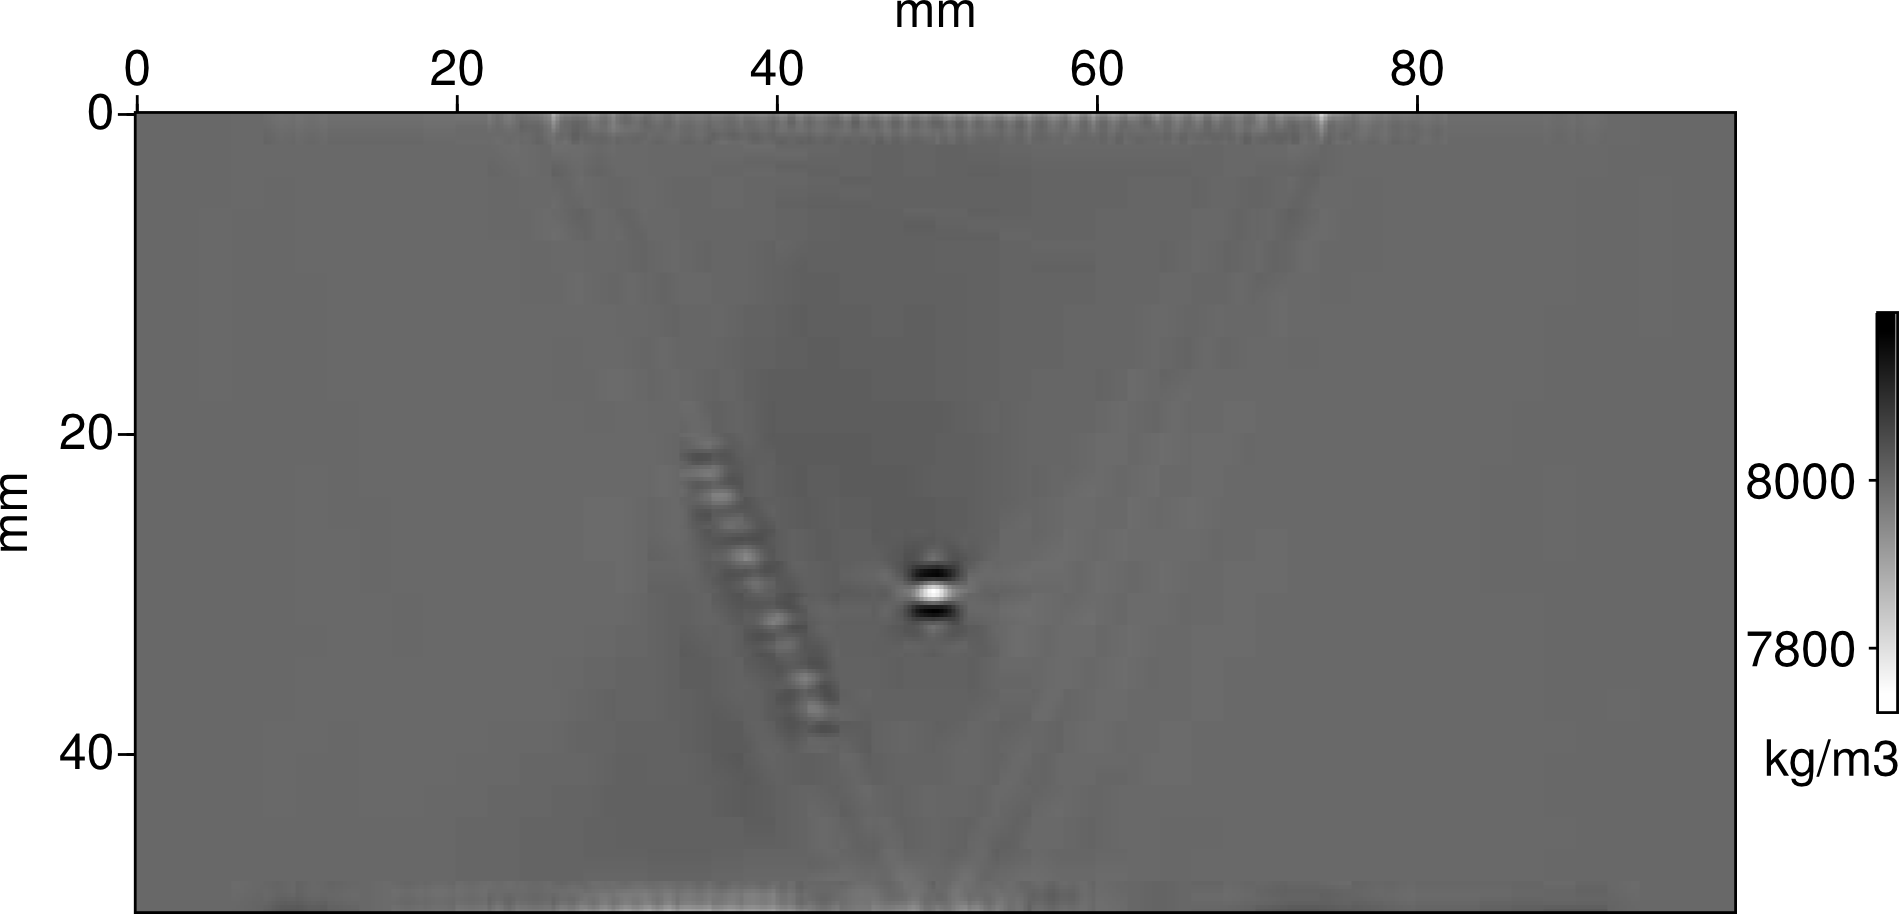
\includegraphics[width=\textwidth]{img/rho_mono/rho_mono.png}\\
%	
%			\column{0.35\textwidth}
%			\centering
%			Masse volumique vraie : \\[0.2cm]
%			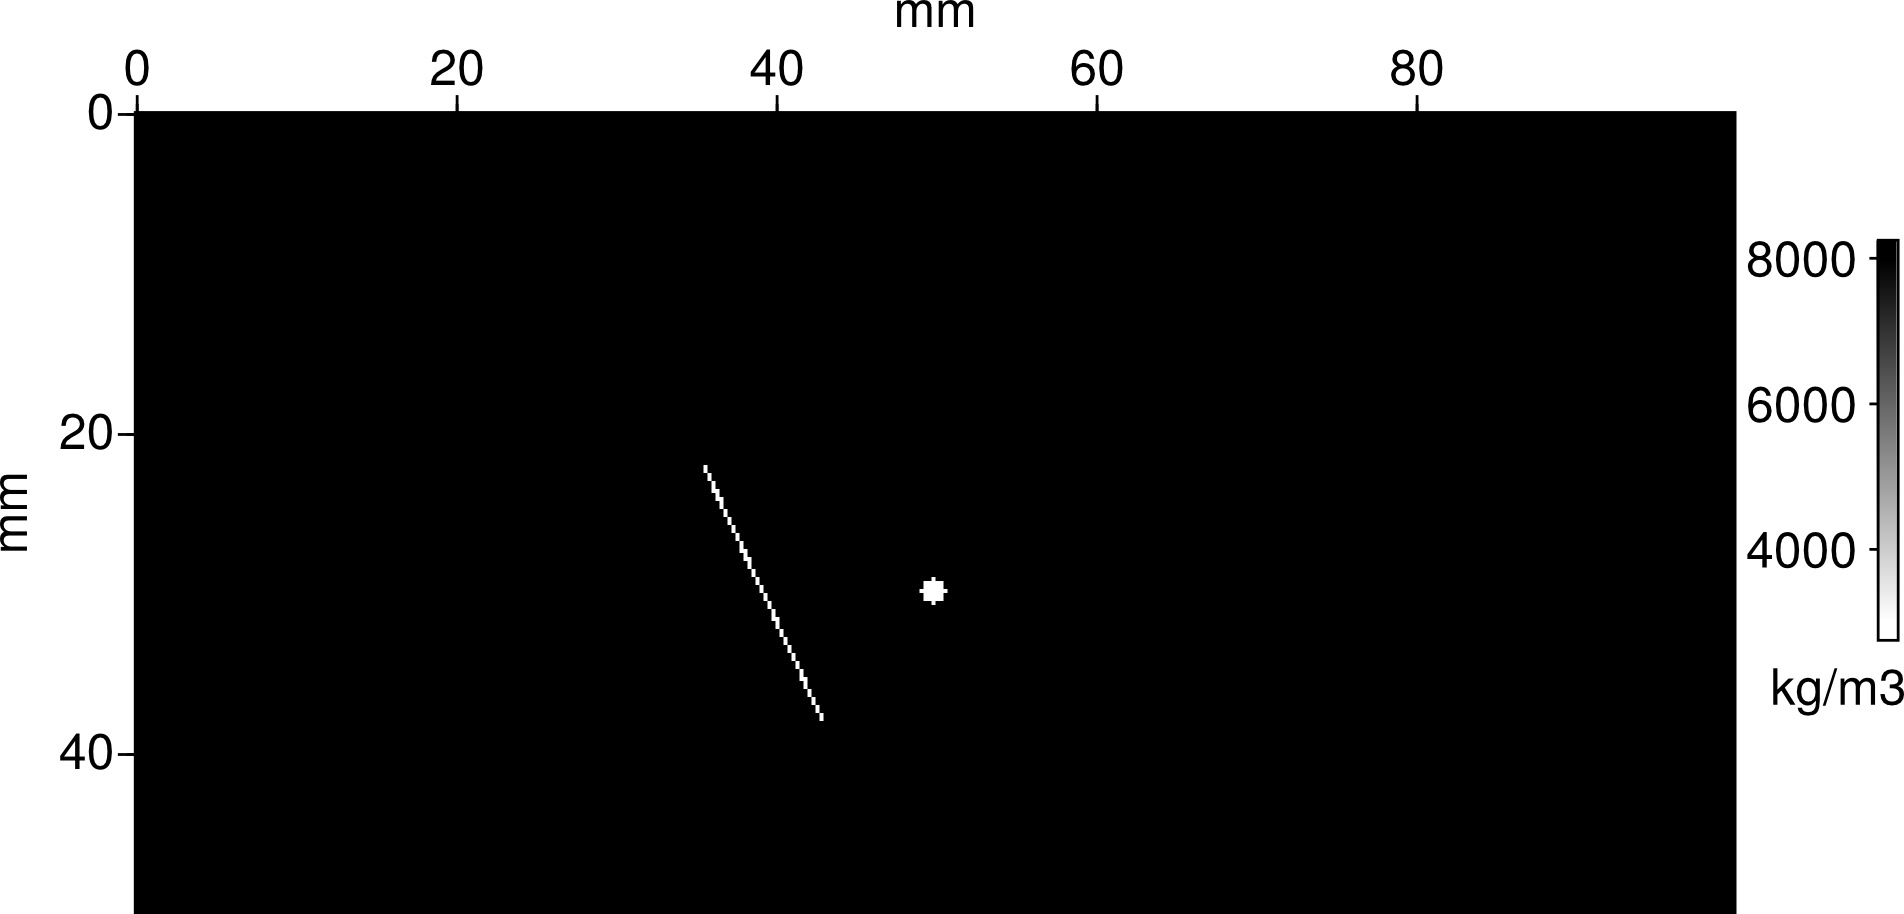
\includegraphics[width=\textwidth]{img/rho_true.png}
%		\end{columns}
%
%\end{footnotesize}		
%\end{frame}


%\subsection{Inversion multiparamètre}
%\begin{frame}{\insertsectionhead~ -- Multiparamètre}
%\begin{small}
%	\centering
%	Vitesse initiale :
%	\begin{figure}
%		\centering
%		\includegraphics[width=0.35\textwidth]{img/vp_mono_smooth/vp_smooth.png}\\
%	\end{figure}
%	
%	\begin{columns}
%		\column{0.5\textwidth}
%		\centering
%		Vitesse reconstruite :\\[0.2cm]
%		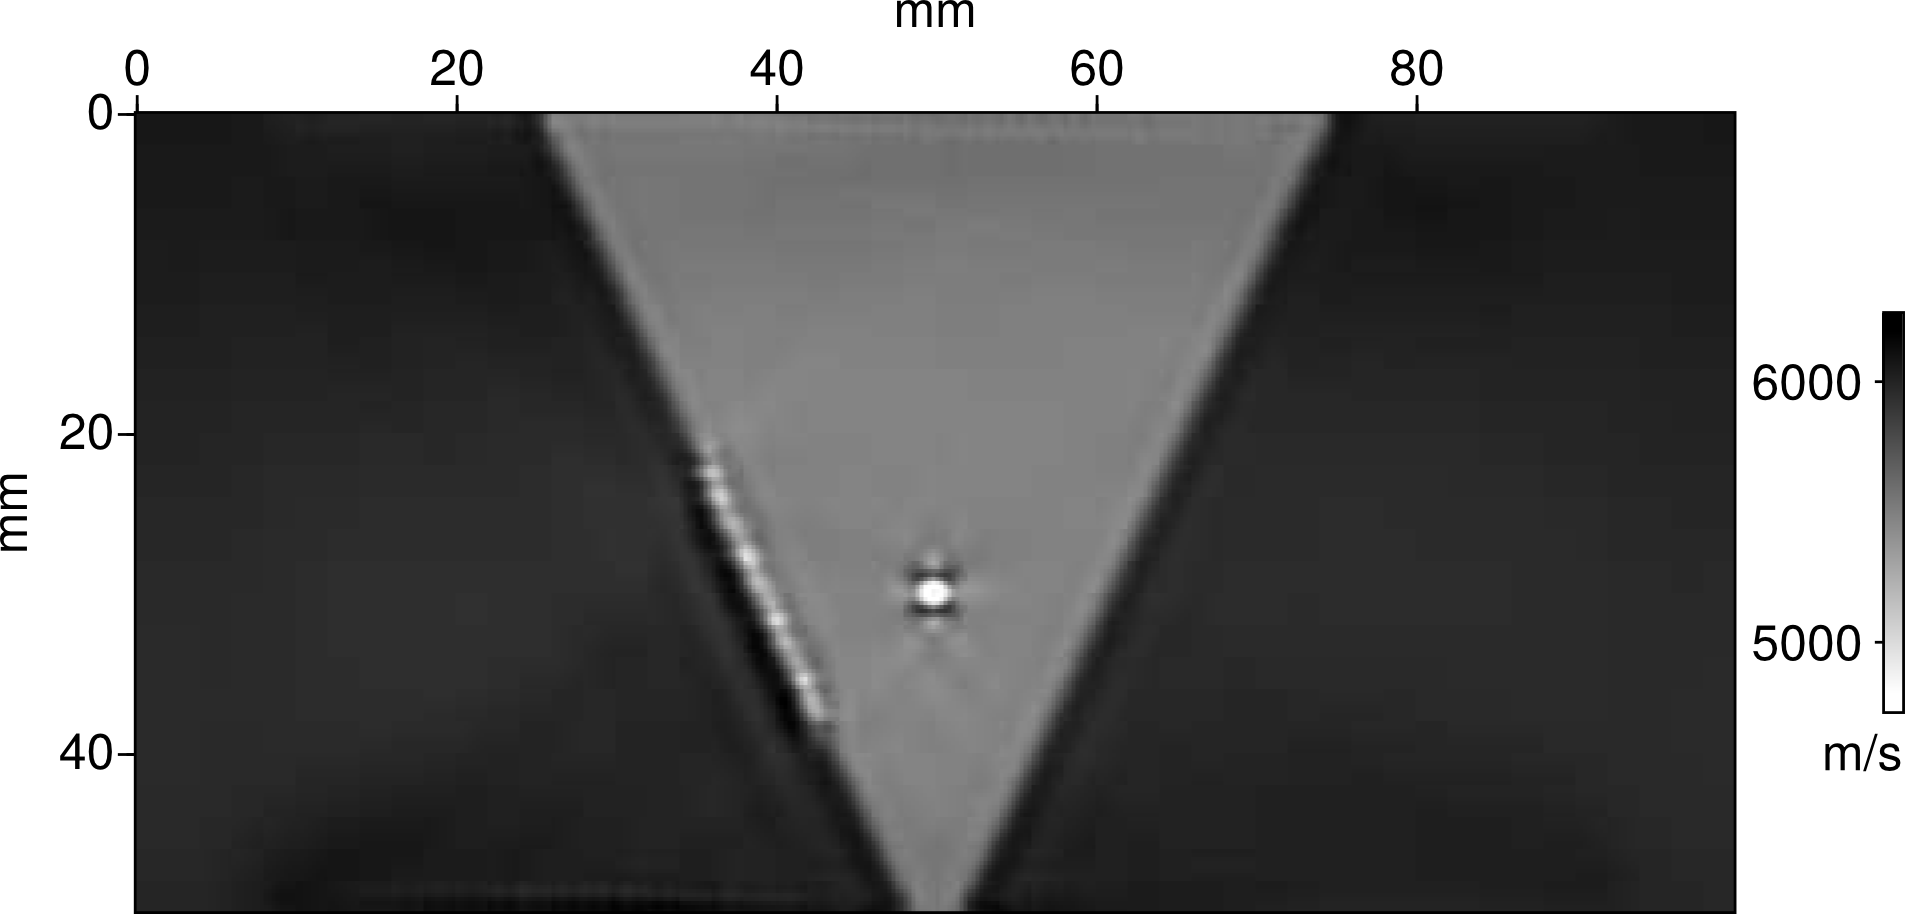
\includegraphics[width=0.7\textwidth]{img/multi/vp_multi_6000k.png}	\\
%		
%		Vitesse vraie : \\[0.2cm]
%		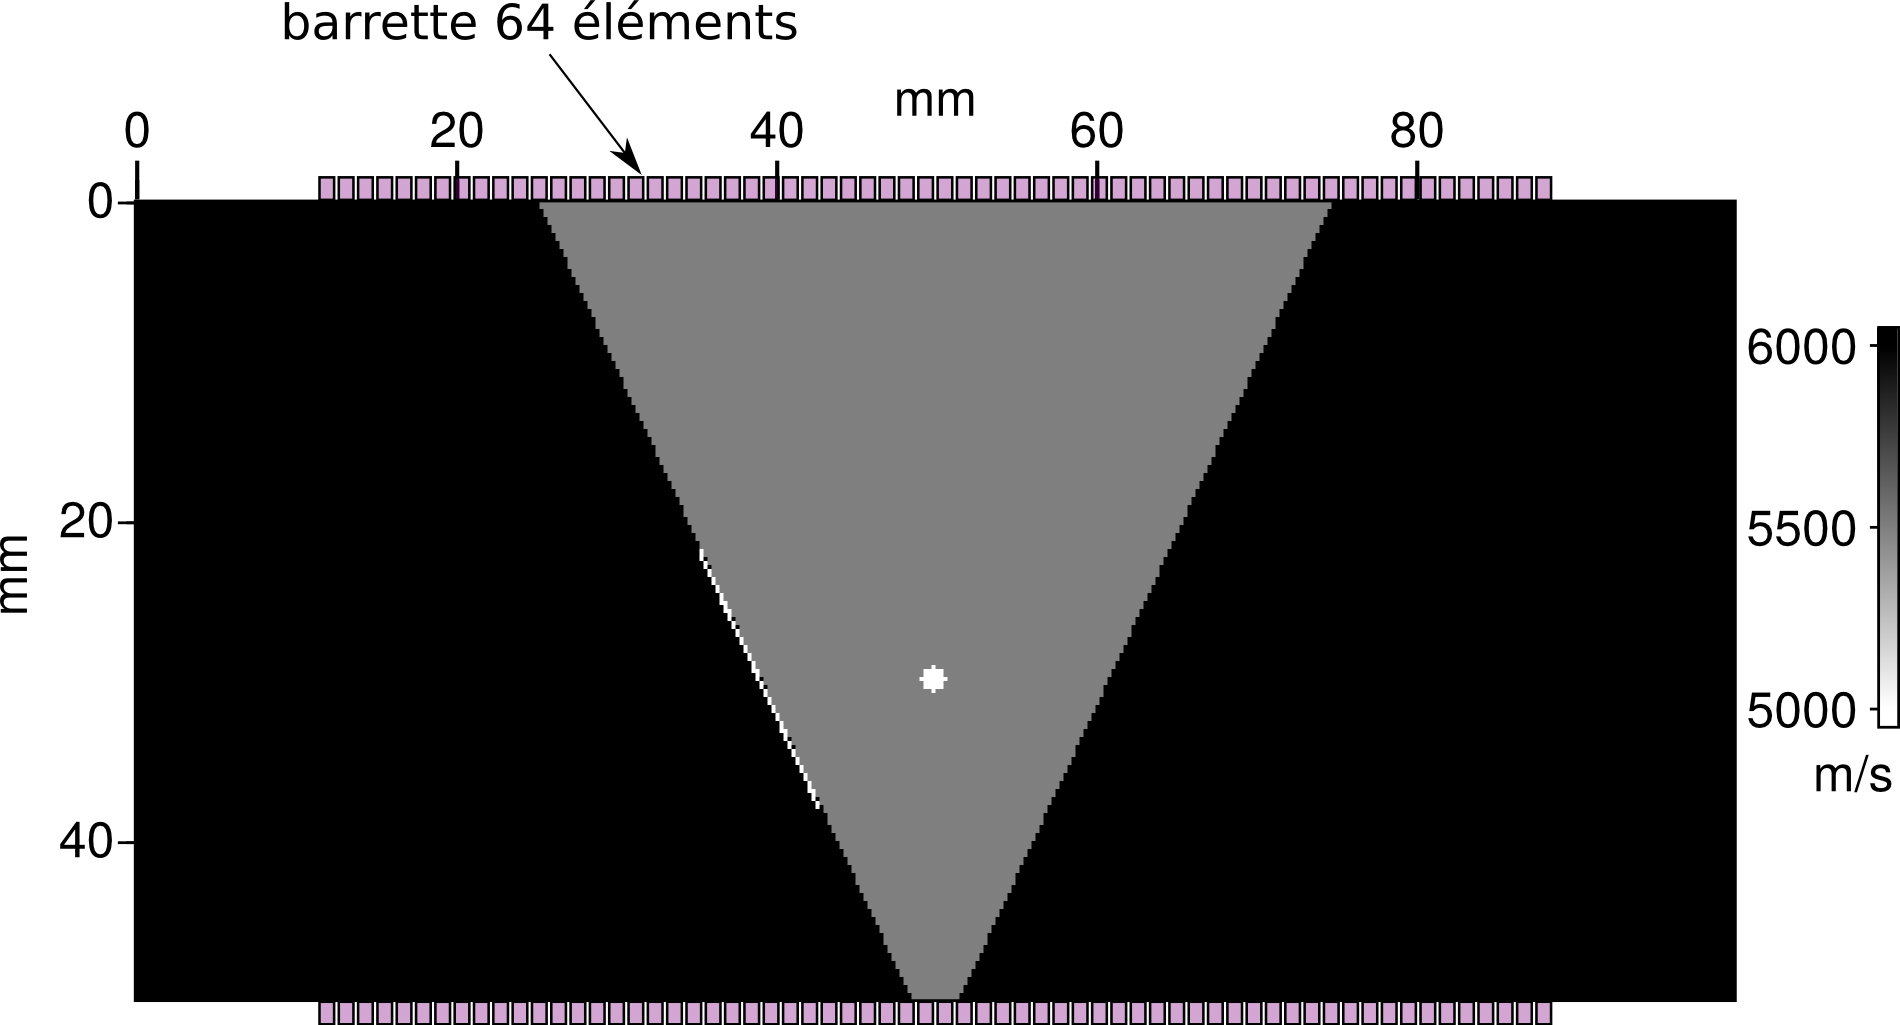
\includegraphics[width=0.7\textwidth]{img/vp_true.png}
%		\column{0.5\textwidth}
%		\centering
%		Masse volumique reconstruite :\\[0.2cm]
%		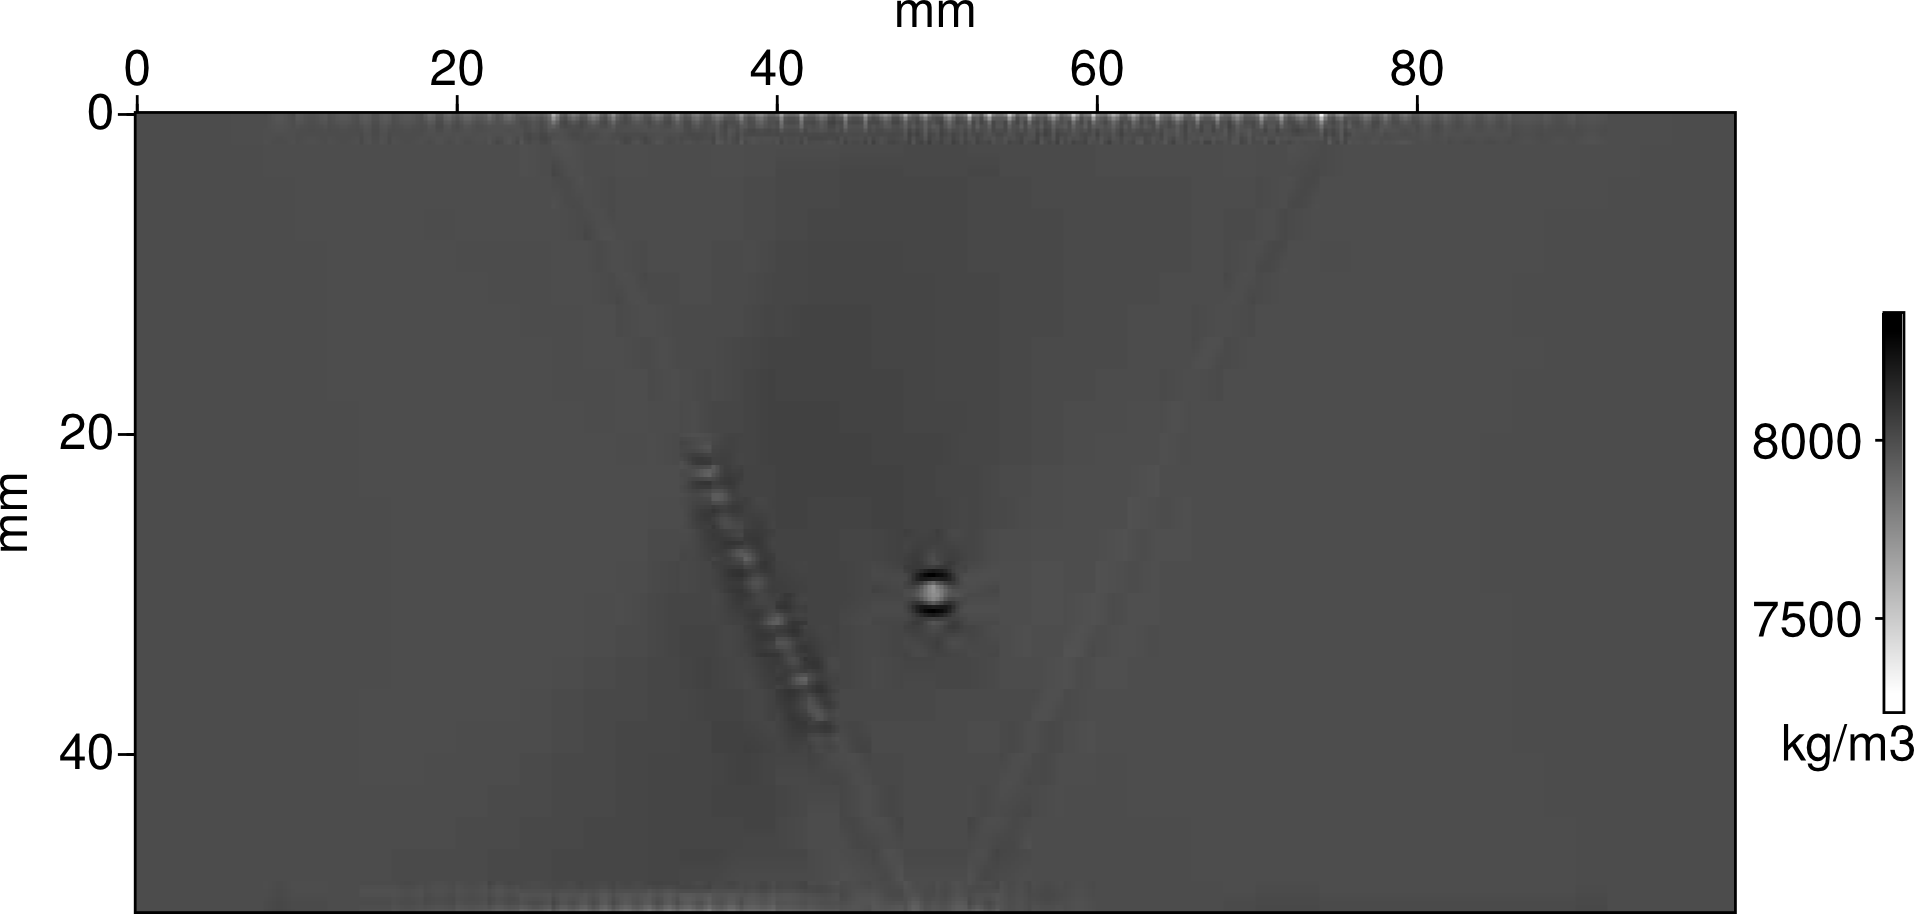
\includegraphics[width=0.7\textwidth]{img/multi/rho_6000k.png}\\	
%		
%		Masse volumique vraie : \\[0.2cm]
%		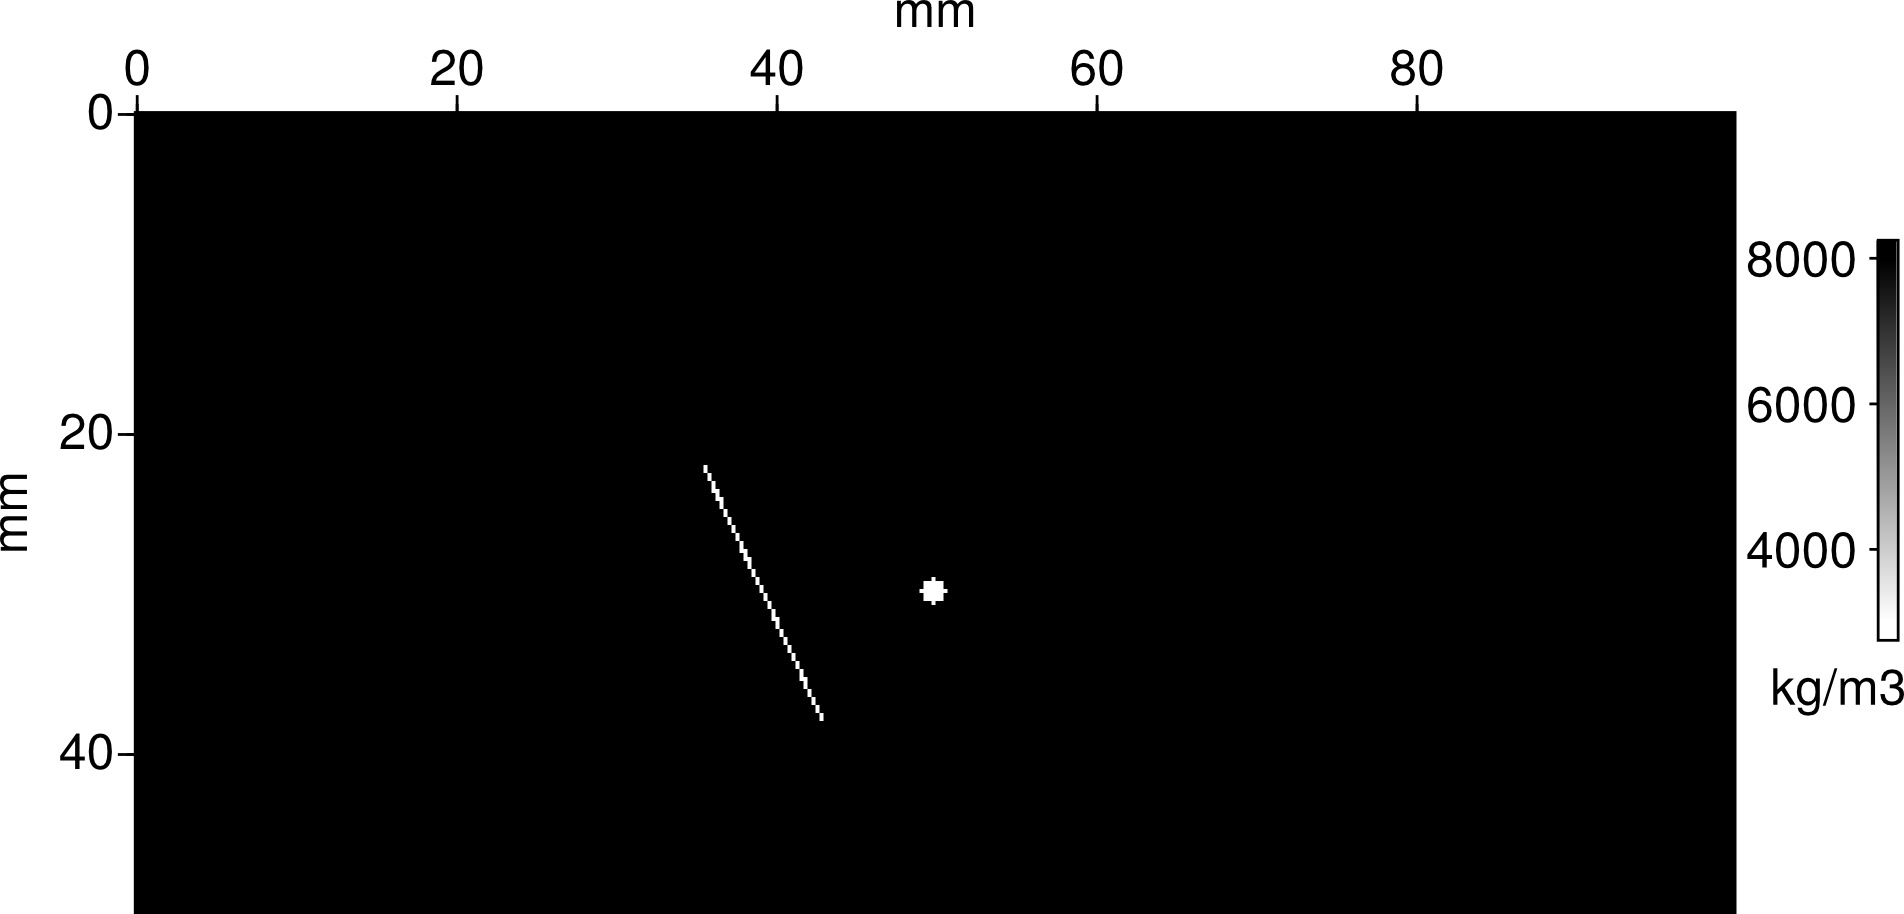
\includegraphics[width=0.7\textwidth]{img/rho_true.png}
%	\end{columns}	
%	
%\end{small}
%\end{frame}


%\subsection{}
\begin{frame}{\insertsectionhead}
\setlength{\leftmargin}{-2cm}
\setlength{\rightmargin}{-2cm}
%\setlength{\textwidth}{29cm}
\begin{picture}(0,0)(0,0)\put(-20,-33){
	$v_{p}$
}\end{picture}
\begin{picture}(0,0)(0,0)\put(-20,-87){
	$\rho$
}\end{picture}
\vspace{-0.5cm}
\begin{itemize}
	\small{\item 9 inversions successives de 200 kHz à 3 MHz }\\[0.3cm]
\end{itemize}
\vspace{0.3cm}
	\begin{columns}
		\column{0.3\textwidth}
		\centering
		\scriptsize{Modèles initiaux}
		\includegraphics[height=1.9cm]{img/vp_mono_smooth/vp_smooth.png}\\
		\includegraphics[height=1.9cm]{img/rho_mono/rho_init.png}		
		\column{0.3\textwidth}
		\centering
		\scriptsize{Inversions monoparamètres}
		\includegraphics[height=1.9cm]{img/vp_mono_uni/vp_3300k.png}\\
		\includegraphics[height=1.9cm]{img/rho_mono/rho_mono.png}		
		\column{0.3\textwidth}
		\centering
		\scriptsize{Inversion multiparamètre}
		\includegraphics[height=1.9cm]{img/multi/vp_multi_6000k.png}\\		
		\includegraphics[height=1.9cm]{img/multi/rho_6000k.png}\\		
	\end{columns}

\end{frame}

%\begin{frame}{\insertsectionhead}
%\begin{small}
%	\begin{itemize}
%		\item<1-> Modèles initiaux : \\[-0.2cm]
%		\begin{columns}
%			\column{0.5\textwidth}
%			\begin{figure}				
%				\centering{
%				\includegraphics[height=1.7cm]{img/vp_mono_smooth/vp_smooth.png}\\
%				\footnotesize{Vitesse}
%				}
%			\end{figure}
%			\column{0.5\textwidth}
%			\begin{figure}				
%				\centering{
%				\includegraphics[height=1.7cm]{img/vp_mono_smooth/rho_init.png}\\
%				\footnotesize{Masse volumique}
%				}
%			\end{figure}
%		\end{columns}
%		\item<2-> Inversions monoparamètres : \\[-0.2cm]
%		\begin{columns}
%			\column{0.5\textwidth}
%			\begin{figure}				
%				\centering{
%				\includegraphics[height=1.7cm]{img/vp_mono_smooth/vp_2900k.png}\\
%				\footnotesize{Vitesse}
%				}
%			\end{figure}
%			\column{0.5\textwidth}
%			\begin{figure}				
%				\centering{
%				\includegraphics[height=1.7cm]{img/rho_mono/rho_mono.png}\\
%				\footnotesize{Masse volumique}
%				}
%			\end{figure}
%		\end{columns}
%		\item<3-> Inversion multiparamètre : \\[-0.2cm]
%		\begin{columns}
%			\column{0.5\textwidth}
%			\begin{figure}				
%				\centering{
%				\includegraphics[height=1.7cm]{img/multi/vp_multi_6000k.png}\\
%				\footnotesize{Vitesse}
%				}
%			\end{figure}
%			\column{0.5\textwidth}
%			\begin{figure}				
%				\centering{
%				\includegraphics[height=1.7cm]{img/multi/rho_6000k.png}\\
%				\footnotesize{Masse volumique}
%				}
%			\end{figure}
%		\end{columns}
%	\end{itemize}
%\end{small}
%\end{frame}


\subsection*{}
\begin{frame}{\insertsectionhead}
\begin{small}
\begin{itemize}
	\item Inversion monoparamètre : \\[0.2cm]
	\begin{columns}
		\column{0.5\textwidth}
		\centering
		Vitesse : \\[0.2cm]
		\includegraphics[width=0.6\textwidth]{img/multi/coupe_vp_mono_smooth_hor.png}\\
		\column{0.5\textwidth}
		\centering
		Masse volumique  : \\[0.2cm]
		\includegraphics[width=0.6\textwidth]{img/multi/coupe_rho_mono.png}\\
	\end{columns}
	\item Inversion multiparamètre : \\[0.2cm]
	\begin{columns}
		\column{0.5\textwidth}
		\centering
		Vitesse : \\[0.2cm]
		\includegraphics[width=0.6\textwidth]{img/multi/coupe_vp_multi.png}\\
		\column{0.5\textwidth}
		\centering
		Masse volumique : \\[0.2cm]
		\includegraphics[width=0.6\textwidth]{img/multi/coupe_rho_multi.png}\\
	\end{columns}
	
\end{itemize}
\hspace{2.7cm}Coupes horizontales à 3 cm de profondeur
\end{small}
\end{frame}

\begin{frame}{\insertsectionhead}
\setlength{\leftmargin}{-2cm}
\setlength{\rightmargin}{-2cm}
%\setlength{\textwidth}{29cm}
\begin{picture}(0,0)(0,0)\put(-20,-33){
	$v_{p}$
}\end{picture}
\begin{picture}(0,0)(0,0)\put(-20,-87){
	$\rho$
}\end{picture}
\vspace{-0.5cm}
\begin{itemize}
	\small{\item 9 inversions successives de 200 kHz à 3 MHz }
\end{itemize}
\vspace{0.3cm}
	\begin{columns}
		\column{0.3\textwidth}
		\centering
		\scriptsize{Modèles initiaux}
		\includegraphics[height=1.9cm]{img/vp_mono_smooth/vp_smooth.png}\\
		\includegraphics[height=1.9cm]{img/rho_mono/rho_init.png}		
		\column{0.3\textwidth}
		\centering
		\scriptsize{Inversions monoparamètres}
		\includegraphics[height=1.9cm]{img/vp_mono_uni/vp_3300k.png}\\
		\includegraphics[height=1.9cm]{img/rho_mono/rho_mono.png}		
		\column{0.3\textwidth}
		\centering
		\scriptsize{Inversion multiparamètre}
		\includegraphics[height=1.9cm]{img/multi/vp_multi_6000k.png}\\		
		\includegraphics[height=1.9cm]{img/multi/rho_6000k.png}\\		
	\end{columns}
	\vspace{0.5cm}
	\onslide<2->{
		\begin{columns}
			\column{0.6\textwidth}
			\small{
			\begin{itemize}
				\item Comparaison avec la méthode FTP\\[0.3cm]
			\end{itemize}
			 \centering
			\begin{equation*}
				I(\bm{r})= \displaystyle\sum_{r} \displaystyle\sum_{e} s_{r,e}\left( T_{\bm{r}\bm{r}_{r}+T_{\bm{r}\bm{r}_{e}}} \right)
			\end{equation*}
			}
			\column{0.4\textwidth}
			\centering
			\includegraphics[height=2.5cm]{img/tfm_retouche.png}
		\end{columns}
	}
\end{frame}

\section{Inversions en milieu anisotrope}
\subsection*{}
\begin{frame}{\insertsectionhead}
%\begin{small}
	%\begin{columns}
		\centering
		%\column{0.5\textwidth}
		%\centering
		\begin{itemize}
			\item  Milieu acoustique, isotrope transverse (axe de symétrie horizontal)
			\item Paramètre d'anisotropie :
		\begin{equation*}
			\epsilon = \frac{\bm{v}_{p}.\bm{e}_{x}-\bm{v}_{p}.\bm{e_{z}}}{\bm{v}_{p}.\bm{e}_{z}}
		\end{equation*}
		%\column{0.3\textwidth}
		%\hspace{-0.5cm}\includegraphics[height=4cm]{img/anisotrope/e20.png}
		%\column{0.3\textwidth}
		%\hspace{-0.3cm}\includegraphics[height=4cm]{img/anisotrope/residu_init.png}
	%\end{columns}	
	\vspace{-0.5cm}
	\begin{columns}
		\column{0.5\textwidth}
		\centering
		$\epsilon$ vrai : \\[0.2cm]
		\includegraphics[width=0.8\textwidth]{img/anisotrope/epsilon_true.png}\\
		
		\column{0.5\textwidth}
		\centering
		$\epsilon$ reconstruit : \\[0.2cm]
		\includegraphics[width=0.8\textwidth]{img/anisotrope/epsilon_final.png}\\
	\end{columns}
	\vspace{0.3cm}
	\item Trajets horizontaux porteurs d'information : $\theta=\pi~~\rightarrow~~k\sim 0$
	\item Modèle peu représentatif
	
	\end{itemize}
		
%\end{small}
\end{frame}


\section{Conclusions et perspectives}
\subsection*{}
\begin{frame}{\insertsectionhead}
\setlength{\leftmargin}{-1cm}
\setlength{\rightmargin}{-1cm}

	\begin{itemize}
		\item<1-> Inversion multiparamètre : corrige les artefacts
		\item<2-> Prise en compte de l'anisotropie : 
		\begin{itemize}
			\item en acoustique : par un modèle isotrope transverse incliné
			\item en élastique : par $6\times C_{ij}$
		\end{itemize} 
		\begin{figure}[!h]
		    \centering
		    \hspace{-1cm}\begin{subfigure}[b]{0.25\textwidth}
		    	\centering
		 		\includegraphics[height=2cm]{img/ogilvy_model.png}
		 		\vspace{0.2cm}\caption{\centering \scriptsize Modèle d'orientation des grains}
			\end{subfigure}
			\begin{subfigure}[b]{0.7\textwidth}
				\centering
		 		\includegraphics[height=2cm]{img/ogilvy_ray1.png}
		 		\includegraphics[height=2cm]{img/ogilvy_ray2.png}\\
		 		\raggedright{\vspace{-0.25cm}\tiny{\itshape Images extraites de~Ogilvy, 1986}}
		 		\caption{\scriptsize Courbure des rayons (ondes de compressions) \\~}
			\end{subfigure}\\
				
		\end{figure}	
		\item<3-> Élaboration d'un modèle initial fiable 
		\item<4-> Géométrie d'acquisition à adapter
			\begin{itemize}
				\item à la géométrie de la soudure réelle
				\item pour une une bonne illumination/résolution
			\end{itemize}
		\item<5-> Prise en compte de la propagation 3D
	\end{itemize}
	\begin{picture}(0,0)(0,0)\put(240,0){
		\only<5->{
		\begin{tikzpicture}
			\node (a) at (0,0) {\includegraphics[width=2.5cm]{img/linear_array.png}};
			\node (b) [below=-0.2cm of a] {\tiny \itshape Image Olympus};
		\end{tikzpicture}
		}
	}\end{picture}
	
\end{frame}


%\begin{frame}[hide,allowframebreaks]{Références}
%
%	\begin{adjustwidth}{-2em}{-2.5em}
%		\scriptsize
%		\bibliographystyle{abbrvnat}
%		\bibliography{biblio}
%	\end{adjustwidth}
%\end{frame}
{
\setbeamercolor{background canvas}{bg=}
\includepdf[pages={1,2}]{annexes.pdf}
}



\end{document}
